\part{Example Models}\label{example-models.part}

\chapter{Regression Models}

\noindent
Stan supports regression models from simple linear regressions to
multilevel generalized linear models.

\section{Linear Regression}

The simplest linear regression model is the following, with a single
predictor and a slope and intercept coefficient, and normally
distributed noise.  This model can be written using standard
regression notation as
%
\[
y_n = \alpha + \beta x_n + \epsilon_n
\ \ \ \mbox{where} \ \ \
\epsilon_n \sim \distro{Normal}(0,\sigma).
\]
This is equivalent to the following sampling involving the
residual,
\[
y_n - (\alpha + \beta X_n) \sim \distro{Normal}(0,\sigma),
\]
and reducing still further, to
\[
y_n \sim \distro{Normal}(\alpha + \beta X_n, \, \sigma).
\]
%
This latter form of the model is coded in Stan as follows.
%
\begin{stancode}
data {
  int<lower=0> N;
  vector[N] x;
  vector[N] y;
}
parameters {
  real alpha;
  real beta;
  real<lower=0> sigma;
}
model {
  y ~ normal(alpha + beta * x, sigma);
}
\end{stancode}
%
There are \code{N} observations, each with predictor \code{x[n]} and
outcome \code{y[n]}.  The intercept and slope parameters are
\code{alpha} and \code{beta}.  The model assumes a normally
distributed noise term with scale \code{sigma}.  This model has
improper priors for the two regression coefficients.

\subsection{Matrix Notation and Vectorization}

The sampling statement in the previous model is vectorized, with
%
\begin{quote}
\begin{Verbatim}
  y ~ normal(alpha + beta * x, sigma);
\end{Verbatim}
\end{quote}
%
providing the same model as the unvectorized version,
%
\begin{stancode}
  for (n in 1:N)
    y[n] ~ normal(alpha + beta * x[n], sigma);
\end{stancode}
%
In addition to being more concise, the vectorized form is much faster.%
%
\footnote{Unlike in Python and R, which are interpreted, Stan is
  translated to \Cpp and compiled, so loops and assignment statements
  are fast.  Vectorized code is faster in Stan because (a) the
  expression tree used to compute derivatives can be simplified,
  leading to fewer virtual function calls, and (b) computations that
  would be repeated in the looping version, such as \code{log(sigma)}
  in the above model, will be computed once and reused.}

In general, Stan allows the arguments to distributions such as
\code{normal} to be vectors.  If any of the other arguments are
vectors or arrays, they have to be the same size.  If any of the other
arguments is a scalar, it is reused for each vector entry.  See
\refsection{vectorization} for more information on vectorization of
probability functions.

The other reason this works is that Stan's arithmetic operators are
overloaded to perform matrix arithmetic on matrices.  In this case,
because \code{x} is of type \code{vector} and \code{beta} of type
\code{real}, the expression \code{beta * x} is of type \code{vector}.
Because Stan supports vectorization, a regression model with more than
one predictor can be written directly using matrix notation.
%
\begin{stancode}
data {
  int<lower=0> N;   // number of data items
  int<lower=0> K;   // number of predictors
  matrix[N, K] x;   // predictor matrix
  vector[N] y;      // outcome vector
}
parameters {
  real alpha;           // intercept
  vector[K] beta;       // coefficients for predictors
  real<lower=0> sigma;  // error scale
}
model {
  y ~ normal(x * beta + alpha, sigma);  // likelihood
}
\end{stancode}
%
The constraint \code{lower=0} in the declaration of \code{sigma}
constrains the value to be greater than or equal to 0.  With no prior
in the model block, the effect is an improper prior on non-negative
real numbers.  Although a more informative prior may be added, improper
priors are acceptable as long as they lead to proper posteriors.

In the model above, \code{x} is an $N \times K$ matrix of predictors
and \code{beta} a $K$-vector of coefficients, so \code{x * beta} is an
$N$-vector of predictions, one for each of the $N$ data items.  These
predictions line up with the outcomes in the $N$-vector \code{y}, so
the entire model may be written using matrix arithmetic as shown.  It
would be possible to include a column of 1 values in \code{x} and
remove the \code{alpha} parameter.

The sampling statement in the model above is just a more efficient,
vector-based approach to coding the model with a loop, as in the
following statistically equivalent model.
%
\begin{stancode}
model {
  for (n in 1:N)
    y[n] ~ normal(x[n] * beta, sigma);
}
\end{stancode}
%
With Stan's matrix indexing scheme, \code{x[n]} picks out row \code{n}
of the matrix \code{x};  because \code{beta} is a column vector,
the product \code{x[n] * beta} is a scalar of type \code{real}.

\subsubsection{Intercepts as Inputs}

In the model formulation
%
\begin{stancode}
  y ~ normal(x * beta, sigma);
\end{stancode}
%
there is no longer an intercept coefficient \code{alpha}.  Instead, we
have assumed that the first column of the input matrix \code{x} is a
column of 1 values.  This way, \code{beta[1]} plays the role of the
intercept.  If the intercept gets a different prior than the slope
terms, then it would be clearer to break it out.  It is also slightly
more efficient in its explicit form with the intercept variable
singled out because there's one fewer multiplications; it should not
make that much of a difference to speed, though, so the choice should
be based on clarity.

\section{The QR Reparameterization}\label{QR-reparameterization.section}

In the previous example, the linear predictor can be written as
$\eta = x \beta$, where $\eta$ is a $N$-vector of predictions,
$x$ is a $N \times K$ matrix, and $\beta$ is a $K$-vector of coefficients.
Presuming $N \geq K$, we can exploit the fact that any design matrix, $x$
can be decomposed using the thin QR decomposition into an orthogonal matrix
$Q$ and an upper-triangular matrix $R$, i.e. $x = Q R$. See \ref{QR-decomposition}
for more information on the QR decomposition but note that \code{qr\_Q} and
\code{qr\_R} implement the fat QR decomposition so here we thin it by including
only $K$ columns in $Q$ and $K$ rows in $R$. Also, in practice, it is best to
write $x = Q^\ast R^\ast$ where $Q^\ast = Q \times \sqrt{n - 1}$ and
$R^\ast = \frac{1}{\sqrt{n - 1}} R$. Thus, we can equivalently write
$\eta = x \beta = Q R \beta = Q^\ast R^\ast \beta$. If we let
$\theta = R^\ast \beta$, then we have $\eta = Q^\ast \theta$ and
$\beta = R^{\ast^{-1}} \theta$. In that case, the previous Stan program becomes
%
\begin{stancode}
data {
  int<lower=0> N;   // number of data items
  int<lower=0> K;   // number of predictors
  matrix[N, K] x;   // predictor matrix
  vector[N] y;      // outcome vector
}
transformed data {
  matrix[N, K] Q_ast;
  matrix[K, K] R_ast;
  matrix[K, K] R_ast_inverse;
  // thin and scale the QR decomposition
  Q_ast = qr_Q(x)[, 1:K] * sqrt(N - 1);
  R_ast = qr_R(x)[1:K, ] / sqrt(N - 1);
  R_ast_inverse = inverse(R_ast);
}
parameters {
  real alpha;           // intercept
  vector[K] theta;      // coefficients on Q_ast
  real<lower=0> sigma;  // error scale
}
model {
  y ~ normal(Q_ast * theta + alpha, sigma);  // likelihood
}
generated quantities {
  vector[K] beta;
  beta = R_ast_inverse * theta; // coefficients on x
}
\end{stancode}
%
Since this Stan program generates equivalent predictions for $y$ and
the same posterior distribution for $\alpha$, $\beta$, and $\sigma$ as
the previous Stan program, many wonder why the version with this QR
reparameterization performs so much better in practice, often both in
terms of wall time and in terms of effective sample size. The
reasoning is threefold:
%
\begin{enumerate}
\item The columns of $Q^\ast$ are orthogonal whereas the columns of
  $x$ generally are not. Thus, it is easier for a Markov Chain to move
  around in $\theta$-space than in $\beta$-space.
\item The columns of $Q^\ast$ have the same scale whereas the columns
  of $x$ generally do not. Thus, a Hamiltonian Monte Carlo algorithm
  can move around the parameter space with a smaller number of larger
  steps
\item Since the covariance matrix for the columns of $Q\ast$ is an
  identity matrix, $\theta$ typically has a reasonable scale if the
  units of $y$ are also reasonable. This also helps HMC move
  efficiently without compromising numerical accuracy.
\end{enumerate}
%
Consequently, this QR reparameterization is recommended for linear and
generalized linear models in Stan whenever $K > 1$ and you do not have
an informative prior on the \emph{location} of $\beta$. It can also be
worthwhile to subtract the mean from each column of $x$ before
obtaining the QR decomposition, which does not affect the posterior
distribution of $\theta$ or $\beta$ but does affect $\alpha$ and
allows you to interpret $\alpha$ as the expectation of $y$ in a linear
model.

\section{Priors for Coefficients and Scales}\label{regression-priors.section}

This section describes the choices available for modeling priors for
regression coefficients and scales.  Priors for univariate parameters
in hierarchical models are discussed in
\refsection{hierarchical-priors} and multivariate parameters in
\refsection{multivariate-hierarchical-priors}. There is also a
discussion of priors used to identify models in
\refsection{priors-for-identification}.

However, as described in \refsection{QR-reparameterization}, if you do
not have an informative prior on the \emph{location} of the regression
coefficients, then you are better off reparameterizing your model so
that the regression coefficients are a generated quantity. In that case,
it usually does not matter very much what prior is used on on the
reparameterized regression coefficients and almost any weakly informative
prior that scales with the outcome will do.

\subsection{Background Reading}

See \citep{Gelman:2006} for an overview of choices for priors for
scale parameters, \citep{ChungEtAl:2013} for an overview of choices
for scale priors in penalized maximum likelihood estimates, and
\cite{GelmanJakulinPittauEtAl:2008} for a discussion of prior choice
for regression coefficients.

\subsection{Improper Uniform Priors}

The default in Stan is to provide uniform (or ``flat'') priors on
parameters over their legal values as determined by their declared
constraints.  A parameter declared without constraints is thus given a
uniform prior on $(-\infty,\infty)$ by default, whereas a scale
parameter declared with a lower bound of zero gets an improper uniform
prior on $(0,\infty)$.  Both of these priors are improper in the sense
that there is no way formulate a density function for them that
integrates to 1 over its support.

Stan allows models to be formulated with improper priors, but in order
for sampling or optimization to work, the data provided must ensure a
proper posterior.  This usually requires a minimum quantity of data,
but can be useful as a starting point for inference and as a baseline
for sensitivity analysis (i.e., considering the effect the prior
has on the posterior).

Uniform priors are specific to the scale on which they are formulated.
For instance, we could give a scale parameter $\sigma > 0$ a uniform
prior on $(0,\infty)$, $q(\sigma) = c$ (we use $q$ because the
``density'' is not only unnormalized, but unnormalizable), or we could
work on the log scale and provide $\log \sigma$ a uniform prior on
$(-\infty,\infty)$, $q(\log \sigma) = c$.  These work out to be
different priors on $\sigma$ due to the Jacobian adjustment necessary
for the log transform; see \refsection{change-of-variables} for more
information on changes of variables and their requisite Jacobian
adjustments.

Stan automatically applies the necessary Jacobian adjustment for
variables declared with constraints to ensure a uniform density on the
legal constrained values.  This Jacobian adjustment is turned off when
optimization is being applied in order to produce appropriate maximum
likelihood estimates.

\subsection{Proper Uniform Priors: Interval Constraints}

It is possible to declare a variable with a proper uniform prior by
imposing both an upper and lower bound on it, for example,
%
\begin{stancode}
real<lower=0.1, upper=2.7> sigma;
\end{stancode}
%
This will implicitly give \code{sigma} a $\distro{Uniform}(0.1, 2.7)$
prior.

\subsubsection{Matching Support to Constraints}

As with all constraints, it is important that the model
provide support for all legal values of \code{sigma}.  For example,
the following code constraints \code{sigma} to be positive, but then
imposes a bounded uniform prior on it.
%
\begin{stancode}
parameters {
  real<lower=0> sigma;
  ...
model {
  // *** bad *** : support narrower than constraint
  sigma ~ uniform(0.1, 2.7);
\end{stancode}
%
The sampling statement imposes a limited support for \code{sigma} in
(0.1, 2.7), which is narrower than the support declared in the
constraint, namely $(0, \infty)$.  This can cause the Stan program to
be difficult to initialize, hang during sampling, or devolve to a
random walk.

\subsubsection{Boundary Estimates}

Estimates near boundaries for interval-constrained parameters
typically signal that the prior is not appropriate for the model.  It
can also cause numerical problems with underflow and overflow when
sampling or optimizing.

\subsection{``Uninformative'' Proper Priors}

It is not uncommon to see models with priors on regression
coefficients such as $\distro{Normal}(0,1000)$.%
%
\footnote{The practice was common in BUGS and can be seen in most of
  their examples \cite{LunnEtAl:2012}.}
%
If the prior scale, such as 1000, is several orders of magnitude
larger than the estimated coefficients, then such a prior is
effectively providing no effect whatsoever.

We actively discourage users from using the default scale priors
suggested through the BUGS examples \citep{LunnEtAl:2012}, such as
\[
\sigma^2 \sim \distro{InvGamma}(0.001, 0.001).
\]
%
Such priors concentrate too much probability mass outside of
reasonable posterior values, and unlike the symmetric wide normal
priors, can have the profound effect of skewing posteriors; see
\citep{Gelman:2006} for examples and discussion.

\subsection{Truncated Priors}

If a variable is declared with a lower bound of zero, then assigning
it a normal prior in a Stan model produces the same effect as
providing a properly truncated half-normal prior.  The truncation at
zero need not be specified as Stan only requires the density up to a
proportion.  So a variable declared with
%
\begin{stancode}
real<lower=0> sigma;
\end{stancode}
%
and given a prior
\begin{stancode}
sigma ~ normal(0, 1000);
\end{stancode}
%
gives \code{sigma} a half-normal prior, technically
%
\[
p(\sigma)
\ = \
\frac{\distro{Normal}(\sigma | 0, 1000)}
     {1 - \distro{NormalCDF}(0 | 0, 1000)}
\ \propto \
\distro{Normal}(\sigma | 0, 1000),
\]
%
but Stan is able to avoid the calculation of the normal cumulative
distribution (CDF) function required to normalize the half-normal density.
If either the prior location or scale is a parameter or if the
truncation point is a parameter, the truncation cannot be dropped,
because the normal CDF term will not be a constant.


\subsection{Weakly Informative Priors}

Typically a researcher will have some knowledge of the scale of the
variables being estimated.  For instance, if we're estimating an
intercept-only model for the mean population height for adult women,
then we know the answer is going to be somewhere in the one to three
meter range.  That gives us information around which to form a weakly
informative prior.

Similarly, a logistic regression with predictors on the standard scale
(roughly zero mean, unit variance) is unlikely to have a
coefficient that's larger than five in absolute value.  In these
cases, it makes sense to provide a weakly informative prior such as
$\distro{Normal}(0,5)$ for such a coefficient.

Weakly informative priors help control inference computationally and
statistically.  Computationally, a prior increases the curvature
around the volume where the solution is expected to lie, which in turn
guides both gradient-based like L-BFGS and Hamiltonian Monte Carlo
sampling by not allowing them to stray too far from the location of a
surface.  Statistically, a weakly informative prior is more sensible
for a problem like women's mean height, because a very diffuse prior
like $\distro{Normal}(0,1000)$ will ensure that the vast majority of
the prior probability mass is outside the range of the expected
answer, which can overwhelm the inferences available from a small data
set.

\subsection{Bounded Priors}

Consider the women's height example again.  One way to formulate a
proper prior is to impose a uniform prior on a bounded scale.  For
example, we could declare the parameter for mean women's height to
have a lower bound of one meter and an upper bound of three meters.
Surely the answer has to lie in that range.

Similarly, it is not uncommon to see priors for scale parameters that
impose lower bounds of zero and upper bounds of very large numbers,
such as 10,000.%
%
\footnote{This was also a popular strategy in the BUGS example models
  \citep{LunnEtAl:2012}, which often went one step further and set the
  lower bounds to a small number like 0.001 to discourage numerical
  underflow to zero.}
%
This provides roughly the same problem for estimation as a very
diffuse inverse gamma prior on variance.  We prefer to leave
parameters which are not absolutely physically constrained to float
and provide them informative priors.  In the case of women's height,
such a prior might be $\distro{Normal}(2,0.5)$ on the scale of meters;
it concentrates 95\% of its mass in the interval $(1,3)$, but still
allows values outside of that region.

In cases where bounded priors are used, the posterior fits should be
checked to make sure the parameter is not estimated at or very close
to a boundary.  This will not only cause computational problems, it
indicates a problem with the way the model is formulated.  In such
cases, the interval should be widened to see where the parameter fits
without such constraints, or boundary-avoid priors should be used (see
\refsection{hierarchical-priors}.)

\subsection{Fat-Tailed Priors and ``Default'' Priors}

A reasonable alternative if we want to accommodate outliers is to use a
prior that concentrates most of mass around the area where values are
expected to be, but still leaves a lot of mass in its tails.  The
usual choice in such a situation is to use a Cauchy distribution for a
prior, which can concentrate its mass around its median, but has tails
that are so fat that the variance is infinite.

Without specific information, the Cauchy prior is a very good default
parameter choice for regression coefficients
\citep{GelmanJakulinPittauEtAl:2008} and the half-Cauchy (coded
implicitly in Stan) a good default choice for scale parameters
\citep{Gelman:2006}.



\subsection{Informative Priors}

Ideally, there will be substantive information about a problem that
can be included in an even tighter prior than a weakly informative
prior.  This may come from actual prior experiments and thus be the
posterior of other data, it may come from meta-analysis, or it may
come simply by soliciting it from domain experts.  All the goodness of
weakly informative priors applies, only with more strength.

\subsection{Conjugacy}

Unlike in Gibbs sampling, there is no computational advantage to
providing conjugate priors (i.e., priors that produce posteriors in
the same family) in a Stan program.%
%
\footnote{BUGS and JAGS both support conjugate sampling through Gibbs
  sampling.  JAGS extended the range of conjugacy that could be
  exploited with its GLM module.  Unlike Stan, both BUGS and JAGS are
  restricted to conjugate priors for constrained multivariate
  quantities such as covariance matrices or simplexes.}
%
Neither the Hamiltonian Monte Carlo samplers or the optimizers make
use of conjugacy, working only on the log density and its derivatives.



\section{Robust Noise Models}

The standard approach to linear regression is to model the noise
term $\epsilon$ as having a normal distribution.  From Stan's
perspective, there is nothing special about normally distributed
noise.  For instance, robust regression can be accommodated by giving
the noise term a Student-$t$ distribution.  To code this in Stan, the
sampling distribution is changed to the following.
%

\begin{stancode}
data {
  ...
  real<lower=0> nu;
}
...
model {
  y ~ student_t(nu, alpha + beta * x, sigma);
}
\end{stancode}
%
The degrees of freedom constant \code{nu} is specified as data.

\section{Logistic and Probit Regression}\label{logistic-probit-regression.section}

For binary outcomes, either of the closely related logistic or probit
regression models may be used.  These generalized linear models vary
only in the link function they use to map linear predictions in
$(-\infty,\infty)$ to probability values in $(0,1)$.  Their respective
link functions, the logistic function and the unit normal cumulative distribution
function, are both sigmoid functions (i.e., they are both {\it S}-shaped).

A logistic regression model with one predictor and an intercept is coded as
follows.
%

\begin{stancode}
data {
  int<lower=0> N;
  vector[N] x;
  int<lower=0,upper=1> y[N];
}
parameters {
  real alpha;
  real beta;
}
model {
  y ~ bernoulli_logit(alpha + beta * x);
}
\end{stancode}
%
The noise parameter is built into the Bernoulli formulation here
rather than specified directly.

Logistic regression is a kind of generalized linear model with binary
outcomes and the log odds (logit) link function, defined by
%
\[
\mbox{logit}(v) = \log \left( \frac{v}{1-v} \right).
\]
%
The inverse of the link function appears in the model.
%
\[
\mbox{logit}^{-1}(u) = \frac{1}{1 + \exp(-u)}.
\]
%

The model formulation above uses the logit-parameterized version of
the Bernoulli distribution, which is defined by
%
\[
\distro{BernoulliLogit}(y|\alpha)
=
\distro{Bernoulli}(y | \mbox{logit}^{-1}(\alpha)).
\]
%
The formulation is also vectorized in the sense that \code{alpha} and
\code{beta} are scalars and \code{x} is a vector, so that \code{alpha
  + beta * x} is a vector.  The vectorized formulation is equivalent
to the less efficient version
%

\begin{stancode}
for (n in 1:N)
  y[n] ~ bernoulli_logit(alpha + beta * x[n]);
\end{stancode}
%
Expanding out the Bernoulli logit, the model is equivalent to the more
explicit, but less efficient and less arithmetically stable
%

\begin{stancode}
for (n in 1:N)
  y[n] ~ bernoulli(inv_logit(alpha + beta * x[n]));
\end{stancode}

Other link functions may be used in the same way.  For example, probit
regression uses the cumulative normal distribution function, which is
typically written as
\[
\Phi(x) = \int_{-\infty}^x \distro{Normal}(y|0,1) \, dy.
\]
%
The cumulative unit normal distribution function $\Phi$ is implemented
in Stan as the function \code{Phi}.  The probit regression model
may be coded in Stan by replacing the logistic model's sampling
statement with the following.
%

\begin{stancode}
        y[n] ~ bernoulli(Phi(alpha + beta * x[n]));
\end{stancode}
%
A fast approximation to the cumulative unit normal distribution function
$\Phi$ is implemented in Stan as the function \code{Phi\_approx}.  The
approximate probit regression model may be coded with the following.
%

\begin{stancode}
        y[n] ~ bernoulli(Phi_approx(alpha + beta * x[n]));
\end{stancode}

\section{Multi-Logit Regression}\label{multi-logit.section}

Multiple outcome forms of logistic regression can be coded directly in
Stan.  For instance, suppose there are $K$ possible outcomes for each
output variable $y_n$.  Also suppose that there is a $D$-dimensional
vector $x_n$ of predictors for $y_n$.  The multi-logit model with
$\distro{Normal}(0,5)$ priors on the coefficients is coded as follows.
%

\begin{stancode}
data {
  int K;
  int N;
  int D;
  int y[N];
  vector[D] x[N];
}
parameters {
  matrix[K,D] beta;
}
model {
  for (k in 1:K)
    beta[k] ~ normal(0, 5);
  for (n in 1:N)
    y[n] ~ categorical(softmax(beta * x[n]));
}
\end{stancode}
%
See \refsection{softmax} for a definition of the softmax
function.   A more efficient way to write the final line is
%
\begin{stancode}
    y[n] ~ categorical_logit(beta * x[n]);
\end{stancode}
%
The \code{categorical\_logit} distribution is like the categorical
distribution, with the parameters on the logit scale (see
\refsection{categorical-distribution} for a full definition of
\code{categorical\_logit}).

The first loop may be made more efficient by vectorizing the first
loop by converting the matrix \code{beta} to a vector,
%
\begin{stancode}
to_vector(beta) ~ normal(0, 5);
\end{stancode}


\subsubsection{Constraints on Data Declarations}

The data block in the above model is defined without constraints on
sizes \code{K}, \code{N}, and \code{D} or on the outcome array
\code{y}.  Constraints on data declarations provide error checking at
the point data is read (or transformed data is defined), which is
before sampling begins.  Constraints on data declarations also make
the model author's intentions more explicit, which can help with
readability.  The above model's declarations could be tightened to
%

\begin{stancode}
  int<lower=2> K;
  int<lower=0> N;
  int<lower=1> D;
  int<lower=1,upper=K> y[N];
\end{stancode}
%
These constraints arise because the number of categories, \code{K},
must be at least two in order for a categorical model to be useful.
The number of data items, \code{N}, can be zero, but not negative;
unlike R, Stan's for-loops always move forward, so that a loop extent
of \code{1:N} when \code{N} is equal to zero ensures the loop's body
will not be executed.  The number of predictors, \code{D}, must be at
least one in order for \code{beta * x[n]} to produce an
appropriate argument for \code{softmax()}.  The categorical outcomes
\code{y[n]} must be between \code{1} and \code{K} in order for the
discrete sampling to be well defined.

Constraints on data declarations are optional.  Constraints on
parameters declared in the \code{parameters} block, on the other hand,
are {\it not}\ optional---they are required to ensure support for all
parameter values satisfying their constraints.  Constraints on
transformed data, transformed parameters, and generated quantities are
also optional.

\subsection{Identifiability}

Because softmax is invariant under adding a constant to each component
of its input, the model is typically only identified if there is a
suitable prior on the coefficients.

An alternative is to use $(K-1)$-vectors by fixing one of them to be
zero. \refsection{partially-known-parameters} discusses how to mix
constants and parameters in a vector.  In the multi-logit case, the
parameter block would be redefined to use $(K-1)$-vectors
%
\begin{stancode}
parameters {
  matrix[K - 1, D] beta_raw;
}
\end{stancode}
%
and then these are transformed to parameters to use in the model.
First, a transformed data block is added before the parameters block
to define a row vector of zero values,
%
\begin{stancode}
transformed data {
  row_vector[D] zeros;
  zeros = rep_row_vector(0, D);
}
\end{stancode}
%
which can then be appended to \code{beta\_row} to produce the
coefficient matrix \code{beta},
%
\begin{stancode}
transformed parameters {
  matrix[K, D] beta;
  beta = append_row(beta_raw, zeros);
}
\end{stancode}
%
See \refsection{matrix-broadcast} for a definition of
\code{rep\_row\_vector} and \refsection{matrix-concatenation} for a
definition of \code{append\_row}.

This is not quite the same model as using $K$-vectors as parameters,
because now the prior only applies to $(K-1)$-vectors.  In practice,
this will cause the maximum likelihood solutions to be different and
also the posteriors to be slightly different when taking priors
centered around zero, as is typical for regression coefficients.

\section{Parameterizing Centered Vectors}

It is often convenient to define a parameter vector $\beta$ that is
centered in the sense of satisfying the sum-to-zero constraint,
%
\[
\sum_{k=1}^K \beta_k = 0.
\]
%
Such a parameter vector may be used to identify a multi-logit
regression parameter vector (see \refsection{multi-logit}), or may be
used for ability or difficulty parameters (but not both) in an IRT
model (see \refsection{item-response-models}).


\subsection{$K-1$ Degrees of Freedom}

There is more than one way to enforce a sum-to-zero constraint on a
parameter vector, the most efficient of which is to define the $K$-th
element as the negation of the sum of the elements $1$ through $K-1$.
%
\begin{stancode}
parameters {
  vector[K-1] beta_raw;
  ...
transformed parameters {
  vector[K] beta;  // centered

  for (k in 1:(K-1)) {
    beta[k] = beta_raw[k];
  }
  beta[K] = -sum(beta_raw);
  ...
\end{stancode}

Placing a prior on \code{beta\_raw} in this parameterization leads to
a subtly different posterior than that resulting from the same prior
on \code{beta} in the original parameterization without the
sum-to-zero constraint.  Most notably, a simple prior on each
component of \code{beta\_raw} produces different results than putting
the same prior on each component of an unconstrained $K$-vector
\code{beta}.  For example, providing a $\distro{Normal}(0,5)$ prior
on \code{beta} will produce a different posterior mode than placing
the same prior on \code{beta\_raw}.


\subsection{Translated and Scaled Simplex}

An alternative approach that's less efficient, but amenable to a
symmetric prior, is to offset and scale a simplex.
%
\begin{stancode}
parameters {
  simplex[K] beta_raw;
  real beta_scale;
  ...
transformed parameters {
  vector[K] beta;
  beta = beta_scale * (beta_raw - 1.0 / K);
  ...
\end{stancode}
%
Given that \code{beta\_raw} sums to 1 because it is a simplex, the
elementwise subtraction of $1 / K$ is guaranteed to sum to zero (note
that the expression \code{1.0 / K} is used rather than \code{1 / K} to
prevent integer arithmetic rounding down to zero).  Because the
magnitude of the elements of the simplex is bounded, a scaling factor
is required to provide \code{beta} with $K$ degrees of freedom
necessary to take on every possible value that sums to zero.

With this parameterization, a Dirichlet prior can be placed on
\code{beta\_raw}, perhaps uniform, and another prior put on
\code{beta\_scale}, typically for ``shrinkage.''


\subsection{Soft Centering}

Adding a prior such as $\beta \sim \distro{Normal}(0,\sigma)$ will provide a kind
of soft centering of a parameter vector $\beta$ by preferring, all
else being equal, that $\sum_{k=1}^K \beta_k = 0$.  This approach is only
guaranteed to roughly center  if $\beta$ and the elementwise addition $\beta + c$
for a scalar constant $c$ produce the same likelihood (perhaps by
another vector $\alpha$ being transformed to $\alpha - c$, as in the
IRT models).  This is another way of achieving a symmetric prior.


\section{Ordered Logistic and Probit Regression}\label{ordered-logistic.section}

Ordered regression for an outcome $y_n \in \setlist{1,\ldots, k}$ with
predictors $x_n \in \reals^D$ is determined by a single coefficient
vector $\beta \in \reals^D$ along with a sequence of cutpoints $c \in
\reals^{K-1}$ sorted so that $c_d < c_{d+1}$.  The discrete output is
$k$ if the linear predictor $x_n \beta$ falls between $c_{k-1}$ and
$c_k$, assuming $c_0 = -\infty$ and $c_K = \infty$.  The noise term is
fixed by the form of regression, with examples for ordered logistic
and ordered probit models.

\subsection{Ordered Logistic Regression}

The ordered logistic model can be coded in Stan using the
\code{ordered} data type for the cutpoints and the built-in
\code{ordered\_logistic} distribution.
%

\begin{stancode}
data {
  int<lower=2> K;
  int<lower=0> N;
  int<lower=1> D;
  int<lower=1,upper=K> y[N];
  row_vector[D] x[N];
}
parameters {
  vector[D] beta;
  ordered[K-1] c;
}
model {
  for (n in 1:N)
    y[n] ~ ordered_logistic(x[n] * beta, c);
}
\end{stancode}
%
The vector of cutpoints \code{c} is declared as \code{ordered[K-1]},
which guarantees that \code{c[k]} is less than \code{c[k+1]}.

If the cutpoints were assigned independent priors, the constraint
effectively truncates the joint prior to support over points that
satisfy the ordering constraint.  Luckily, Stan does not need to
compute the effect of the constraint on the normalizing term because
the probability is needed only up to a proportion.


\subsubsection{Ordered Probit}

An ordered probit model could be coded in exactly the same way by
swapping the cumulative logistic (\code{inv\_logit}) for the cumulative
normal (\code{Phi}).
%

\begin{stancode}
data {
  int<lower=2> K;
  int<lower=0> N;
  int<lower=1> D;
  int<lower=1,upper=K> y[N];
  row_vector[D] x[N];
}
parameters {
  vector[D] beta;
  ordered[K-1] c;
}
model {
  vector[K] theta;
  for (n in 1:N) {
    real eta;
    eta = x[n] * beta;
    theta[1] = 1 - Phi(eta - c[1]);
    for (k in 2:(K-1))
      theta[k] = Phi(eta - c[k-1]) - Phi(eta - c[k]);
    theta[K] = Phi(eta - c[K-1]);
    y[n] ~ categorical(theta);
  }
}
\end{stancode}
%
The logistic model could also be coded this way by replacing
\code{Phi} with \code{inv\_logit}, though the built-in encoding based
on the softmax transform is more efficient and more numerically
stable.  A small efficiency gain could be achieved by computing the
values \code{Phi(eta - c[k])} once and storing them for re-use.


\section{Hierarchical Logistic Regression}

The simplest multilevel model is a hierarchical model in which the
data is grouped into $L$ distinct categories (or levels).  An extreme
approach would be to completely pool all the data and estimate a
common vector of regression coefficients $\beta$.  At the other
extreme, an approach with no pooling assigns each level $l$ its own
coefficient vector $\beta_l$ that is estimated separately from the
other levels.  A hierarchical model is an intermediate solution where
the degree of pooling is determined by the data and a prior on the
amount of pooling.

Suppose each binary outcome $y_n \in \setlist{0,1}$ has an associated
level, $ll_n \in \setlist{1,\ldots,L}$.  Each outcome will also have
an associated predictor vector $x_n \in \reals^D$.  Each level $l$
gets its own coefficient vector $\beta_l \in \reals^D$.  The
hierarchical structure involves drawing the coefficients $\beta_{l,d}
\in \reals$ from a prior that is also estimated with the data.  This
hierarchically estimated prior determines the amount of pooling.  If
the data in each level are very similar, strong pooling will be
reflected in low hierarchical variance.  If the data in the levels are
dissimilar, weaker pooling will be reflected in higher hierarchical variance.

The following model encodes a hierarchical logistic regression model
with a hierarchical prior on the regression coefficients.
%

\begin{stancode}
data {
  int<lower=1> D;
  int<lower=0> N;
  int<lower=1> L;
  int<lower=0,upper=1> y[N];
  int<lower=1,upper=L> ll[N];
  row_vector[D] x[N];
}
parameters {
  real mu[D];
  real<lower=0> sigma[D];
  vector[D] beta[L];
}
model {
  for (d in 1:D) {
    mu[d] ~ normal(0, 100);
    for (l in 1:L)
      beta[l,d] ~ normal(mu[d], sigma[d]);
  }
  for (n in 1:N)
    y[n] ~ bernoulli(inv_logit(x[n] * beta[ll[n]]));
}
\end{stancode}
%
The standard deviation parameter \code{sigma} gets an implicit uniform
prior on $(0,\infty)$ because of its declaration with a lower-bound
constraint of zero.  Stan allows improper priors as long as the
posterior is proper.  Nevertheless, it is usually helpful to have
informative or at least weakly informative priors for all parameters;
see \refsection{regression-priors} for recommendations on priors for
regression coefficients and scales.

\subsubsection{Optimizing the Model}

Where possible, vectorizing sampling statements leads to faster log
probability and derivative evaluations.  The speed boost is not
because loops are eliminated, but because vectorization allows sharing
subcomputations in the log probability and gradient calculations and
because it reduces the size of the expression tree required for
gradient calculations.

The first optimization vectorizes the for-loop over \code{D} as
%

\begin{stancode}
  mu ~ normal(0, 100);
  for (l in 1:L)
    beta[l] ~ normal(mu, sigma);
\end{stancode}
%
The declaration of \code{beta} as an array of vectors means that the
expression \code{beta[l]} denotes a vector.  Although \code{beta}
could have been declared as a matrix, an array of vectors (or a
two-dimensional array) is more efficient for accessing rows; see
\refsection{indexingefficiency} for more information on the efficiency
tradeoffs among arrays, vectors, and matrices.

This model can be further sped up and at the same time made more
arithmetically stable by replacing the application of inverse-logit
inside the Bernoulli distribution with the logit-parameterized
Bernoulli,
%

\begin{stancode}
  for (n in 1:N)
    y[n] ~ bernoulli_logit(x[n] * beta[ll[n]]);
\end{stancode}
%
See \refsection{bernoulli-logit-distribution} for a definition of
\code{bernoulli\_logit}.

Unlike in R or BUGS, loops, array access and assignments are fast in
Stan because they are translated directly to \Cpp.  In most cases, the
cost of allocating and assigning to a container is more than made up
for by the increased efficiency due to vectorizing the log probability
and gradient calculations.  Thus the following version is faster than
the original formulation as a loop over a sampling statement.
%

\begin{stancode}
  {
    vector[N] x_beta_ll;
    for (n in 1:N)
      x_beta_ll[n] = x[n] * beta[ll[n]];
    y ~ bernoulli_logit(x_beta_ll);
  }
\end{stancode}
%
The brackets introduce a new scope for the local variable
\code{x\_beta\_ll}; alternatively, the variable may be declared at the
top of the model block.

In some cases, such as the above, the local variable assignment leads
to models that are less readable.  The recommended practice in such
cases is to first develop and debug the more transparent version of
the model and only work on optimizations when the simpler formulation
has been debugged.


\section{Hierarchical Priors}\label{hierarchical-priors.section}

Priors on priors, also known as ``hyperpriors,'' should be treated the
same way as priors on lower-level parameters in that as much prior
information as is available should be brought to bear.  Because
hyperpriors often apply to only a handful of lower-level parameters,
care must be taken to ensure the posterior is both proper and not
overly sensitive either statistically or computationally to wide tails
in the priors.

\subsection{Boundary-Avoiding Priors for MLE in Hierarchical Models}

The fundamental problem with maximum likelihood estimation (MLE) in
the hierarchical model setting is that as the hierarchical variance
drops and the values cluster around the hierarchical mean, the overall
density grows without bound.  As an illustration, consider a simple
hierarchical linear regression (with fixed prior mean) of $y_n \in
\reals$ on $x_n \in \reals^K$, formulated as
%
\begin{eqnarray*}
y_n & \sim & \distro{Normal}(x_n \beta, \sigma)
\\[3pt]
\beta_k & \sim & \distro{Normal}(0,\tau)
\\[3pt]
\tau & \sim & \distro{Cauchy}(0,2.5)
\end{eqnarray*}
%
In this case, as $\tau \rightarrow 0$ and $\beta_k \rightarrow 0$, the
posterior density
\[
p(\beta,\tau,\sigma|y,x) \propto p(y|x,\beta,\tau,\sigma)
\]
grows without bound.  There is a plot of a Neal's funnel density in
\reffigure{funnel}, which has similar behavior.

There is obviously no MLE estimate for $\beta,\tau,\sigma$ in such a
case, and therefore the model must be modified if posterior modes are
to be used for inference.  The approach recommended by
\cite{ChungEtAl:2013} is to use a gamma distribution as a prior, such
as
%
\[
\sigma \sim \distro{Gamma}(2, 1/A),
\]
%
for a reasonably large value of $A$, such as $A = 10$.


\section{Item-Response Theory Models}\label{item-response-models.section}

Item-response theory (IRT) models the situation in which a number of
students each answer one or more of a group of test questions.  The
model is based on parameters for the ability of the students, the
difficulty of the questions, and in more articulated models, the
discriminativeness of the questions and the probability of guessing
correctly; see \citep[pps.~314--320]{GelmanHill:2007} for a textbook
introduction to hierarchical IRT models and \citep{Curtis:2010} for
encodings of a range of IRT models in BUGS.


\subsection{Data Declaration with Missingness}

The data provided for an IRT model may be declared as follows
to account for the fact that not every student is required to answer
every question.
%

\begin{stancode}
data {
  int<lower=1> J;              // number of students
  int<lower=1> K;              // number of questions
  int<lower=1> N;              // number of observations
  int<lower=1,upper=J> jj[N];  // student for observation n
  int<lower=1,upper=K> kk[N];  // question for observation n
  int<lower=0,upper=1> y[N];   // correctness for observation n
}
\end{stancode}
%
This declares a total of \code{N} student-question pairs in the data
set, where each \code{n} in \code{1:N} indexes a binary observation
\code{y[n]} of the correctness of the answer of student \code{jj[n]}
on question \code{kk[n]}.

The prior hyperparameters will be hard coded in the rest of this
section for simplicity, though they could be coded as data in
Stan for more flexibility.

\subsection{1PL (Rasch) Model}

The 1PL item-response model, also known as the Rasch model, has one
parameter (1P) for questions and uses the logistic link function (L).%
%


The model parameters are declared as follows.
%

\begin{stancode}
parameters {
  real delta;         // mean student ability
  real alpha[J];      // ability of student j - mean ability
  real beta[K];       // difficulty of question k
}
\end{stancode}
%
The parameter \code{alpha[j]} is the ability coefficient for student
\code{j} and \code{beta[k]} is the difficulty coefficient for question
\code{k}.  The non-standard parameterization used here also includes
an intercept term \code{delta}, which represents the average student's
response to the average question.%
%
\footnote{\citep{GelmanHill:2007} treat the $\delta$ term equivalently
  as the location parameter in the distribution of student abilities.}
%
The model itself is as follows.
%

\begin{stancode}
model {
  alpha ~ normal(0, 1);         // informative true prior
  beta ~ normal(0, 1);          // informative true prior
  delta ~ normal(0.75, 1);      // informative true prior
  for (n in 1:N)
    y[n] ~ bernoulli_logit(alpha[jj[n]] - beta[kk[n]] + delta);
}
\end{stancode}
%
This model uses the logit-parameterized Bernoulli distribution, where
\[
\code{bernoulli\_logit}(y|\alpha) =
\code{bernoulli}(y|\mbox{logit}^{-1}(\alpha)).
\]
%
The key to understanding it is the term inside the
\code{bernoulli\_logit} distribution, from which it follows that
\[
\mbox{Pr}[y_n = 1] = \mbox{logit}^{-1}(\alpha_{jj[n]} - \beta_{kk[n]}
+ \delta).
\]
%
The model suffers from additive identifiability issues without the
priors.  For example, adding a term $\xi$ to each $\alpha_j$ and
$\beta_k$ results in the same predictions.  The use of priors for
$\alpha$ and $\beta$ located at 0 identifies the parameters; see
\citep{GelmanHill:2007} for a discussion of identifiability issues and
alternative approaches to identification.

For testing purposes, the IRT 1PL model distributed with Stan uses
informative priors that match the actual data generation process used
to simulate the data in R (the simulation code is supplied in the same
directory as the models).  This is unrealistic for most practical
applications, but allows Stan's inferences to be validated.  A simple
sensitivity analysis with fatter priors shows that the posterior is
fairly sensitive to the prior even with 400 students and 100 questions
and only 25\% missingness at random.  For real applications, the
priors should be fit hierarchically along with the other parameters,
as described in the next section.


\subsection{Multilevel 2PL Model}

The simple 1PL model described in the previous section is generalized
in this section with the addition of a discrimination parameter to
model how noisy a question is and by adding multilevel priors for the
question difficulty and discrimination parameters.  The model
parameters are declared as follows.
%

\begin{stancode}
parameters {
  real mu_beta;                  // mean student ability
  real alpha[J];               // ability for j - mean
  real beta[K];                // difficulty for k
  real<lower=0> gamma[K];      // discrimination of k
  real<lower=0> sigma_beta;    // scale of difficulties
  real<lower=0> sigma_gamma;   // scale of log discrimination
}
\end{stancode}
%
The parameters should be clearer after the model definition.
%
\begin{stancode}
model {
  alpha ~ normal(0, 1);
  beta ~ normal(0, sigma_beta);
  gamma ~ lognormal(0, sigma_gamma);
  mu_beta ~ cauchy(0, 5);
  sigma_alpha ~ cauchy(0, 5);
  sigma_beta ~ cauchy(0, 5);
  sigma_gamma ~ cauchy(0, 5);
  for (n in 1:N)
    y[n] ~ bernoulli_logit(gamma[kk[n]]
                           * (alpha[jj[n]] - (beta[kk[n]] + mu_beta)));
}
\end{stancode}
%
This is similar to the 1PL model, with the additional parameter
\code{gamma[k]} modeling how discriminative question \code{k} is.  If
\code{gamma[k]} is greater than 1, responses are more attenuated with
less chance of getting a question right at random.  The parameter
\code{gamma[k]} is constrained to be positive, which prohibits there
being questions that are easier for students of lesser ability;  such
questions are not unheard of, but they tend to be eliminated from most
testing situations where an IRT model would be applied.

The model is parameterized here with student abilities \code{alpha}
being given a unit normal prior.  This is to identify both the scale
and the location of the parameters, both of which would be
unidentified otherwise; see \refchapter{problematic-posteriors} for
further discussion of identifiability. The difficulty and
discrimination parameters \code{beta} and \code{gamma} then have
varying scales given hierarchically in this model.  They could also be
given weakly informative non-hierarchical priors, such as
%
\begin{stancode}
  beta ~ normal(0, 5);
  gamma ~ lognormal(0, 2);
\end{stancode}
%
The point is that the \code{alpha} determines the scale and location
and \code{beta} and \code{gamma} are allowed to float.

The \code{beta} parameter is here given a non-centered
parameterization, with parameter \code{mu\_beta} serving as the mean
\code{beta} location. An alternative would've been to take:
%
\begin{stancode}
  beta ~ normal(mu_beta, sigma_beta);
\end{stancode}
%
and
%
\begin{stancode}
  y[n] ~ bernoulli_logit(gamma[kk[n]] * (alpha[jj[n]] - beta[kk[n]]));
\end{stancode}
%
Non-centered parameterizations tend to be more efficient in
hierarchical models; see \refsection{reparameterization} for more
information on non-centered reparameterizations.

The intercept term \code{mu\_beta} can't itself be modeled
hierarchically, so it is given a weakly informative
$\distro{Cauchy}(0,5)$ prior.  Similarly, the scale terms,
\code{sigma\_alpha}, \code{sigma\_beta}, and \code{sigma\_gamma}, are
given half-Cauchy priors.  The truncation in the half-Cauchy prior is
implicit; explicit truncation is not necessary because the log
probability need only be calculated up to a proportion and the scale
variables are constrained to $(0,\infty)$ by their declarations.



\section{Priors for Identifiability}\label{priors-for-identification.section}

\subsection{Location and Scale Invariance}

One application of (hierarchical) priors is to identify the scale
and/or location of a group of parameters. For example, in the IRT
models discussed in the previous section, there is both a location and
scale non-identifiability.  With uniform priors, the posteriors will
float in terms of both scale and location.  See
\refsection{collinearity} for a simple example of the problems this
poses for estimation.

The non-identifiability is resolved by providing a unit normal (i.e.,
$\distro{Normal}(0,1)$) prior on one group of coefficients, such as
the student abilities.  With a unit normal prior on the student
abilities, the IRT model is identified in that the posterior will
produce a group of estimates for student ability parameters that have
a sample mean of close to zero and a sample variance of close to one.
The difficulty and discrimination parameters for the questions should
then be given a diffuse, or ideally a hierarchical prior, which will
identify these parameters by scaling and locating relative to the
student ability parameters.

\subsection{Collinearity}

Another case in which priors can help provide identifiability is in
the case of collinearity in a linear regression.  In linear
regression, if two predictors are collinear (i.e, one is a linear
function of the other), then their coefficients will have a
correlation of 1 (or -1) in the posterior.  This leads to
non-identifiability.  By placing normal priors on the coefficients,
the maximum likelihood solution of two duplicated predictors (trivially
collinear) will be half the value than would be obtained by only
including one.

\subsection{Separability}

In a logistic regression, if a predictor is positive in cases of 1
outcomes and negative in cases of 0 outcomes, then the maximum
likelihood estimate for the coefficient for that predictor diverges to
infinity.  This divergence can be controlled by providing a prior for
the coefficient, which will ``shrink'' the estimate back toward zero
and thus identify the model in the posterior.

Similar problems arise for sampling with improper flat priors.  The
sampler will try to draw very large values.  By providing a prior,
the posterior will be concentrated around finite values, leading to
well-behaved sampling.



\section{Multivariate Priors for Hierarchical Models}\label{multivariate-hierarchical-priors.section}

In hierarchical regression models (and other situations), several
individual-level variables may be assigned hierarchical priors.  For
example, a model with multiple varying intercepts and slopes within
might assign them a multivariate prior.

As an example, the individuals might be people and the outcome income,
with predictors such as education level and age, and the groups might be states
or other geographic divisions.  The effect of education level and age
as well as an intercept might be allowed to vary by state.
Furthermore, there might be state-level predictors, such as average
state income and unemployment level.

\subsection{Multivariate Regression Example}

\cite[Chapter 13, Chapter 17]{GelmanHill:2007} discuss a hierarchical
model with $N$ individuals organized into $J$ groups.  Each individual
has a predictor row vector $x_n$ of size $K$; to unify the notation, they
assume that $x_{n,1} = 1$ is a fixed ``intercept'' predictor.  To
encode group membership, they assume individual $n$ belongs to group
$jj[n] \in 1{:}J$.  Each individual $n$ also has an observed outcome
$y_n$ taking on real values.

\subsubsection{Likelihood}

The model is a linear regression with slope and intercept coefficients
varying by group, so that $\beta_j$ is the coefficient $K$-vector for
group $j$.  The likelihood function for individual $n$ is then just
%
\[
y_n \sim \distro{Normal}(x_n \, \beta_{jj[n]}, \, \sigma)
\mbox{ for } n \in 1{:}N.
\]
%

\subsubsection{Coefficient Prior}

Gelman and Hill model the coefficient vectors $\beta_j$ as being drawn
from a multivariate distribution with mean vector $\mu$ and
covariance matrix $\Sigma$,%
%
\[
\beta_j \sim \distro{MultiNormal}(\mu, \, \Sigma)
\mbox{ for } j \in 1{:}J.
\]
%
Below, we discuss the full model of Gelman and Hill, which uses
group-level predictors to model $\mu$; for now, we assume $\mu$ is a
simple vector parameter.

\subsubsection{Hyperpriors}

For hierarchical modeling, the group-level mean vector $\mu$ and
covariance matrix $\Sigma$ must themselves be given priors.  The
group-level mean vector can be given a reasonable weakly-informative
prior for independent coefficients, such as
%
\[
\mu_j \sim \distro{Normal}(0,5).
\]
Of course, if more is known about the expected coefficient values
$\beta_{j, k}$, this information can be incorporated into the prior for
$\mu_k$.

For the prior on the covariance matrix, Gelman and Hill suggest using
a scaled inverse Wishart.  That choice was motivated primarily by
convenience as it is conjugate to the multivariate likelihood function
and thus simplifies Gibbs sampling.

In Stan, there is no restriction to conjugacy for multivariate priors,
and we in fact recommend a slightly different approach.  Like Gelman
and Hill, we decompose our prior into a scale and a matrix, but are
able to do so in a more natural way based on the actual variable
scales and a correlation matrix.  Specifically, we define
\[
\Sigma = \mbox{diag\_matrix}(\tau) \ \Omega \ \mbox{diag\_matrix}(\tau),
\]
where $\Omega$ is a correlation matrix and $\tau$ is the vector of
coefficient scales.   This mapping from scale vector $\tau$ and
correlation matrix $\Omega$ can be inverted, using
\[
\tau_k = \sqrt{\, \Sigma_{k,k}}
\]
and
\[
\Omega_{i, j} = \frac{\Sigma_{i, j}}{\tau_i \, \tau_j}.
\]

The components of the scale vector $\tau$ can be given any reasonable
prior for scales, but we recommend something weakly informative like a
half-Cauchy distribution with a small scale, such as
\[
\tau_k \sim \distro{Cauchy}(0, 2.5)
\mbox{ for } k \in 1{:}K \mbox{ constrained by } \tau_k > 0.
\]
As for the prior means, if there is information about the scale of
variation of coefficients across groups, it should be incorporated
into the prior for $\tau$.  For large numbers of exchangeable
coefficients, the components of $\tau$ itself (perhaps excluding the
intercept) may themselves be given a hierarchical prior.

Our final recommendation is to give the correlation matrix $\Omega$ an
LKJ prior with shape $\nu \geq 1$,
\[
\Omega \sim \distro{LKJCorr}(\nu).
\]
The LKJ correlation distribution is defined in
\refsection{lkj-correlation}, but the basic idea for modeling is that
as $\nu$ increases, the prior increasingly concentrates around the
unit correlation matrix (i.e., favors less correlation among the
components of $\beta_{j}$).  At $\nu = 1$, the LKJ correlation
distribution reduces to the identity distribution over correlation
matrices.  The LKJ prior may thus be used to control the expected
amount of correlation among the parameters $\beta_j$.

\subsubsection{Group-Level Predictors for Prior Mean}

To complete Gelman and Hill's model, suppose each group $j \in 1{:}J$
is supplied with an $L$-dimensional row-vector of group-level
predictors $u_j$.  The prior mean for the $\beta_j$ can then itself be
modeled as a regression, using an $L$-dimensional coefficient vector
$\gamma$.  The prior for the group-level coefficients then becomes
\[
\beta_j \sim \distro{MultiNormal}(u_j \, \gamma, \Sigma)
\]

The group-level coefficients $\gamma$ may themselves be given
independent weakly informative priors, such as
\[
\gamma_l \sim \distro{Normal}(0,5).
\]
As usual, information about the group-level means should be
incorporated into this prior.


\subsubsection{Coding the Model in Stan}

The Stan code for the full hierarchical model with multivariate priors
on the group-level coefficients and group-level prior means follows
its definition.
%
\begin{stancode}
data {
  int<lower=0> N;              // num individuals
  int<lower=1> K;              // num ind predictors
  int<lower=1> J;              // num groups
  int<lower=1> L;              // num group predictors
  int<lower=1,upper=J> jj[N];  // group for individual
  matrix[N, K] x;               // individual predictors
  row_vector[L] u[J];          // group predictors
  vector[N] y;                 // outcomes
}
parameters {
  corr_matrix[K] Omega;        // prior correlation
  vector<lower=0>[K] tau;      // prior scale
  matrix[L, K] gamma;           // group coeffs
  vector[K] beta[J];           // indiv coeffs by group
  real<lower=0> sigma;         // prediction error scale
}
model {
  tau ~ cauchy(0, 2.5);
  Omega ~ lkj_corr(2);
  to_vector(gamma) ~ normal(0, 5);
  {
    row_vector[K] u_gamma[J];
    for (j in 1:J)
      u_gamma[j] = u[j] * gamma;
    beta ~ multi_normal(u_gamma, quad_form_diag(Omega, tau));
  }
  for (n in 1:N)
    y[n] ~ normal(x[n] * beta[jj[n]], sigma);
}
\end{stancode}
%
The hyperprior covariance matrix is defined implicitly through the
a quadratic form in the code
because the correlation matrix \code{Omega} and scale vector
\code{tau} are more natural to inspect in the output; to output
\code{Sigma}, define it as a transformed parameter.  The function
\code{quad\_form\_diag} is defined so that
\code{quad\_form\_diag(Sigma,~tau)} is equivalent to
\code{diag\_matrix(tau) * Sigma * diag\_matrix(tau)}, where
\code{diag\_matrix(tau)} returns the matrix with \code{tau} on the
diagonal and zeroes off diagonal; the version using
\code{quad\_form\_diag} should be faster.  See
\refsection{matrix-arithmetic-operators} for more information on
specialized matrix operations.

\subsubsection{Optimization through Vectorization}

The code in the Stan program above can be sped up dramatically by replacing:
%
\begin{stancode}
  for (n in 1:N)
    y[n] ~ normal(x[n] * beta[jj[n]], sigma);
\end{stancode}
%
with the vectorized form:
%
\begin{stancode}
  {
    vector[N] x_beta_jj;
    for (n in 1:N)
      x_beta_jj[n] = x[n] * beta[jj[n]];
    y ~ normal(x_beta_jj, sigma);
  }
\end{stancode}
%
The outer brackets create a local scope in which to define the
variable \code{x\_beta\_jj}, which is then filled in a loop and used
to define a vectorized sampling statement.  The reason this is such a
big win is that it allows us to take the log of sigma only once and it
greatly reduces the size of the resulting expression graph by packing
all of the work into a single density function.

Although it is tempting to redeclare \code{beta} and include a revised
model block sampling statement,
%
\begin{stancode}
parameters {
  matrix[J, K] beta;
...
model {
  y ~ normal(rows_dot_product(x, beta[jj]), sigma);
  ...
\end{stancode}
%
this fails because it breaks the vectorization of sampling for
\code{beta},%
%
\footnote{Thanks to Mike Lawrence for pointing this out in the GitHub
  issue for the manual.}
%
\begin{stancode}
  beta ~ multi_normal(...);
\end{stancode}
%
which requires \code{beta} to be an array of vectors.  Both
vectorizations are important, so the best solution is to just use the
loop above, because \code{rows\_dot\_product} cannot do much
optimization in and of itself because there are no shared computations.

The code in the Stan program above also builds up an array of vectors
for the outcomes and for the multivariate normal, which provides a
very significant speedup by reducing the number of linear systems that
need to be solved and differentiated.
%
\begin{stancode}
  {
    matrix[K, K] Sigma_beta;
    Sigma_beta = quad_form_diag(Omega, tau);
    for (j in 1:J)
      beta[j] ~ multi_normal((u[j] * gamma)', Sigma_beta);
  }
\end{stancode}
%
In this example, the covariance matrix \code{Sigma\_beta} is defined
as a local variable so as not to have to repeat the quadratic form
computation $J$ times.  This vectorization can be combined with the
Cholesky-factor optimization in the next section.

\subsubsection{Optimization through Cholesky Factorization}

The multivariate normal density and LKJ prior on correlation matrices
both require their matrix parameters to be factored.  Vectorizing, as
in the previous section, ensures this is only done once for each
density.  An even better solution, both in terms of efficiency and
numerical stability, is to parameterize the model directly in terms of
Cholesky factors of correlation matrices using the multivariate
version of the non-centered parameterization.  For the model in the
previous section, the program fragment to replace the full matrix
prior with an equivalent Cholesky factorized prior is as follows.
%
\begin{stancode}
data {
  matrix[J, L] u;
  ...
parameters {
  matrix[K, J] z;
  cholesky_factor_corr[K] L_Omega;
  ...
transformed parameters {
  matrix[J, K] beta;
  beta = u * gamma + (diag_pre_multiply(tau,L_Omega) * z)';
}
model {
  to_vector(z) ~ normal(0, 1);
  L_Omega ~ lkj_corr_cholesky(2);
  ...
\end{stancode}
%
The data variable \code{u} was originally an array of vectors, which
is efficient for access; here it is redeclared as a matrix in order to
use it in matrix arithmetic.  The new parameter \code{L\_Omega} is
the Cholesky factor of the original correlation matrix \code{Omega},
so that
%
\begin{stancode}
Omega = L_Omega * L_Omega'
\end{stancode}
%
The prior scale vector \code{tau} is unchanged, and furthermore,
Pre-multiplying the Cholesky factor by the scale produces the Cholesky
factor of the final covariance matrix,
%
\begin{stancode}
  Sigma_beta
  = quad_form_diag(Omega, tau)
  = diag_pre_multiply(tau, L_Omega) * diag_pre_multiply(tau, L_Omega)'
\end{stancode}
%
where the diagonal pre-multiply compound operation is defined by
%
\begin{stancode}
diag_pre_multiply(a, b) = diag_matrix(a) * b
\end{stancode}
%
The new variable \code{z} is declared as a matrix, the entries of
which are given independent unit normal priors; the \code{to\_vector}
operation turns the matrix into a vector so that it can be used as a
vectorized argument to the univariate normal density.  Multiplying the
Cholesky factor of the covariance matrix by \code{z} and adding the
mean \code{(u\,*\,gamma)'} produces a \code{beta} distributed as in
the original model.

Omitting the data declarations, which are the same as before, the
optimized model is as follows.
%
\begin{stancode}
parameters {
  matrix[K, J] z;
  cholesky_factor_corr[K] L_Omega;
  vector<lower=0,upper=pi()/2>[K] tau_unif;
  matrix[L, K] gamma;                         // group coeffs
  real<lower=0> sigma;                       // prediction error scale
}
transformed parameters {
  matrix[J, K] beta;
  vector<lower=0>[K] tau;     // prior scale
  for (k in 1:K) tau[k] = 2.5 * tan(tau_unif[k]);
  beta = u * gamma + (diag_pre_multiply(tau,L_Omega) * z)';
}
model {
  to_vector(z) ~ normal(0, 1);
  L_Omega ~ lkj_corr_cholesky(2);
  to_vector(gamma) ~ normal(0, 5);
  y ~ normal(rows_dot_product(beta[jj] , x), sigma);
}
\end{stancode}

This model also reparameterizes the prior scale \code{tau} to avoid potential problems with the heavy tails of the Cauchy distribution. The statement \code{tau\_unif ~ uniform(0,pi()/2)} can be omitted from the model block because stan increments the log posterior for parameters with uniform priors without it.

% \begin{quote}
% \begin{stancode}
% parameters {
%   vector[3] mu;
%   matrix[3, M] z;
%   cholesky_factor_corr[3] L_Sigma;
%   vector<lower=0>[3] sigma_Sigma;
%   ...
% transformed parameters {
%   matrix[M,3] alpha;
%   alpha
%     = transpose(rep_matrix(mu, M)
%                  + diag_pre_multiply(sigma_Sigma,L_Sigma) * z);
%   ...
% model {
%   to_vector(z) ~ normal(0, 1);
%   gamma ~ normal(0, 5);
%   sigma_Sigma ~ cauchy(0, 2.5);
%   L_Sigma ~ lkj_corr_cholesky(3);
%   ...
% \end{stancode}
% \end{quote}
% %
% Taken together, this Stan program amounts to
% %
% \begin{eqnarray*}
% \sigma & \sim & \mbox{Cauchy}(0, 2.5)
% \\[3pt]
% \Omega & \sim & \mbox{Lkj}(3)
% \\[3pt]
% \Sigma & = & \mbox{diag}(\sigma) \times \Omega \times \mbox{diag}(\sigma)
% \\[3pt]
% \alpha_m & \sim & \mbox{MultiNormal}(\mu, \Sigma)
% \end{eqnarray*}



\section{Prediction, Forecasting, and Backcasting}

Stan models can be used for ``predicting'' the values of arbitrary
model unknowns.  When predictions are about the future, they're called
``forecasts;'' when they are predictions about the past, as in climate
reconstruction or cosmology, they are sometimes called ``backcasts''
(or ``aftcasts'' or ``hindcasts'' or ``antecasts,'' depending on the
author's feelings about the opposite of ``fore'').

\subsection{Programming Predictions}

As a simple example, the following linear regression provides the same
setup for estimating the coefficients \code{beta} as in our very first
example above, using \code{y} for the \code{N} observations and
\code{x} for the \code{N} predictor vectors.  The model parameters and
model for observations are exactly the same as before.

To make predictions, we need to be given the number of predictions,
\code{N\_new}, and their predictor matrix, \code{x\_new}.  The
predictions themselves are modeled as a parameter \code{y\_new}.  The
model statement for the predictions is exactly the same as for the
observations, with the new outcome vector \code{y\_new} and prediction
matrix \code{x\_new}.
%
\begin{stancode}
data {
  int<lower=1> K;
  int<lower=0> N;
  matrix[N, K] x;
  vector[N] y;

  int<lower=0> N_new;
  matrix[N_new, K] x_new;
}
parameters {
  vector[K] beta;
  real<lower=0> sigma;

  vector[N_new] y_new;                  // predictions
}
model {
  y ~ normal(x * beta, sigma);          // observed model

  y_new ~ normal(x_new * beta, sigma);  // prediction model
}
\end{stancode}


\subsection{Predictions as Generated Quantities}

Where possible, the most efficient way to generate predictions is to
use the generated quantities block.  This provides proper Monte Carlo
(not Markov chain Monte Carlo) inference, which can have a much higher
effective sample size per iteration.
%
\begin{stancode}
...data as above...

parameters {
  vector[K] beta;
  real<lower=0> sigma;
}
model {
  y ~ normal(x * beta, sigma);
}
generated quantities {
  vector[N_new] y_new;
  for (n in 1:N_new)
    y_new[n] = normal_rng(x_new[n] * beta, sigma);
}
\end{stancode}
%
Now the data is just as before, but the parameter \code{y\_new} is now
declared as a generated quantity, and the prediction model is
removed from the model and replaced by a pseudo-random draw from a
normal distribution.

\subsubsection{Overflow in Generated Quantities}

It is possible for values to overflow or underflow in generated
quantities.  The problem is that if the result is NaN, then any
constraints placed on the variables will be violated.  It is possible
to check a value assigned by an RNG and reject it if it overflows, but
this is both inefficient and leads to biased posterior estimates.
Instead, the conditions causing overflow, such as trying to generate a
negative binomial random variate with a mean of $2^{31}$.  These must
be intercepted and dealt with, typically be reparameterizing or
reimplementing the random number generator using real values rather
than integers, which are upper-bounded by $2^{31} - 1$ in Stan.


\section{Multivariate Outcomes}

Most regressions are set up to model univariate observations (be they
scalar, boolean, categorical, ordinal, or count).  Even multinomial
regressions are just repeated categorical regressions.  In contrast,
this section discusses regression when each observed value is
multivariate.  To relate multiple outcomes in a regression setting,
their error terms are provided with covariance structure.

This section considers two cases, seemingly unrelated regressions for
continuous multivariate quantities and multivariate probit regression
for boolean multivariate quantities.

\subsection{Seemingly Unrelated Regressions}

The first model considered is the ``seemingly unrelated'' regressions
(SUR) of econometrics where several linear regressions share
predictors and use a covariance error structure rather than
independent errors \citep{Zellner:1962,Greene:2011}.

The model is easy to write down as a regression,
%
\begin{eqnarray*}
 y_n & = & x_n \, \beta + \epsilon_n
\\[4pt]
 \epsilon_n & \sim & \distro{MultiNormal}(0, \Sigma)
\end{eqnarray*}
%
where $x_n$ is a $J$-row-vector of predictors ($x$ is an $(N \times
J)$-matrix), $y_n$ is a $K$-vector of observations, $\beta$ is a $(K
\times J)$-matrix of regression coefficients (vector $\beta_k$ holds
coefficients for outcome $k$), and $\Sigma$ is covariance matrix
governing the error.  As usual, the intercept can be rolled into $x$
as a column of ones.

The basic Stan code is straightforward (though see below for more
optimized code for use with LKJ priors on correlation).
%
\begin{stancode}
data {
  int<lower=1> K;
  int<lower=1> J;
  int<lower=0> N;
  vector[J] x[N];
  vector[K] y[N];
}
parameters {
  matrix[K, J] beta;
  cov_matrix[K] Sigma;
}
model {
  vector[K] mu[N];
  for (n in 1:N)
    mu[n] = beta * x[n];
  y ~ multi_normal(mu, Sigma);
}
\end{stancode}
%
For efficiency, the multivariate normal is vectorized by precomputing
the array of mean vectors and sharing the same covariance matrix.

Following the advice in \refsection{multivariate-hierarchical-priors},
we will place a weakly informative normal prior on the regression
coefficients, an LKJ prior on the correlations and a half-Cauchy prior
on standard deviations.  The covariance structure is parameterized in
terms of Cholesky factors for efficiency and arithmetic stability.
%
\begin{stancode}
...
parameters {
  matrix[K, J] beta;
  cholesky_factor_corr[K] L_Omega;
  vector<lower=0>[K] L_sigma;
}
model {
  vector[K] mu[N];
  matrix[K, K] L_Sigma;

  for (n in 1:N)
    mu[n] = beta * x[n];

  L_Sigma = diag_pre_multiply(L_sigma, L_Omega);

  to_vector(beta) ~ normal(0, 5);
  L_Omega ~ lkj_corr_cholesky(4);
  L_sigma ~ cauchy(0, 2.5);

  y ~ multi_normal_cholesky(mu, L_Sigma);
}
\end{stancode}
%
The Cholesky factor of the covariance matrix is then reconstructed as
a local variable and used in the model by scaling the Cholesky factor
of the correlation matrices. The regression coefficients get a prior
all at once by converting the matrix \code{beta} to a vector.

If required, the full correlation or covariance matrices may be
reconstructed from their Cholesky factors in the generated quantities
block.


\subsection{Multivariate Probit Regression}

The multivariate probit model generates sequences of boolean variables
by applying a step function to the output of a seemingly unrelated
regression.

The observations $y_n$ are $D$-vectors of boolean values (coded 0 for
false, 1 for true).  The values for the observations $y_n$ are based
on latent values $z_n$ drawn from a seemingly unrelated regression
model (see the previous section),
%
\begin{eqnarray*}
 z_n & = & x_n \, \beta + \epsilon_n
\\[4pt]
 \epsilon_n & \sim & \distro{MultiNormal}(0, \Sigma)
\end{eqnarray*}
%
These are then put through the step function to produce a $K$-vector $z_n$
of boolean values with elements defined by
\[
y_{n, k} = \mathrm{I}(z_{n, k} > 0),
\]
where $\mathrm{I}()$ is the indicator function taking the value 1 if its
argument is true and 0 otherwise.

Unlike in the seemingly unrelated regressions case, here the
covariance matrix $\Sigma$ has unit standard deviations (i.e., it is a
correlation matrix).  As with ordinary probit and logistic
regressions, letting the scale vary causes the model (which is defined
only by a cutpoint at 0, not a scale) to be unidentified (see
\citep{Greene:2011}).

Multivariate probit regression can be coded in Stan using the trick
introduced by \cite{AlbertChib:1993}, where the underlying continuous
value vectors $y_n$ are coded as truncated parameters.  The key to
coding the model in Stan is declaring the latent vector $z$ in two
parts, based on whether the corresponding value of $y$ is 0 or 1.
Otherwise, the model is identical to the seemingly unrelated
regression model in the previous section.

First, we introduce a sum function for two-dimensional arrays of
integers;  this is going to help us calculate how many total 1 values
there are in $y$.
%
\begin{stancode}
functions {
  int sum(int[,] a) {
    int s = 0;
    for (i in 1:size(a))
      s += sum(a[i]);
    return s;
  }
}
\end{stancode}
%
The function is trivial, but it's not a built-in for Stan and it's easier to
understand the rest of the model if it's pulled into its own function
so as not to create a distraction.

The data declaration block is much like for the seemingly unrelated
regressions, but the observations \code{y} are now integers
constrained to be 0 or 1.
%
\begin{stancode}
data {
  int<lower=1> K;
  int<lower=1> D;
  int<lower=0> N;
  int<lower=0,upper=1> y[N,D];
  vector[K] x[N];
}
\end{stancode}

After declaring the data, there is a rather involved transformed data
block whose sole purpose is to sort the data array \code{y} into
positive and negative components, keeping track of indexes so that
\code{z} can be easily reassembled in the transformed parameters
block.
%
\begin{stancode}
transformed data {
  int<lower=0> N_pos;
  int<lower=1,upper=N> n_pos[sum(y)];
  int<lower=1,upper=D> d_pos[size(n_pos)];
  int<lower=0> N_neg;
  int<lower=1,upper=N> n_neg[(N * D) - size(n_pos)];
  int<lower=1,upper=D> d_neg[size(n_neg)];

  N_pos = size(n_pos);
  N_neg = size(n_neg);
  {
    int i;
    int j;
    i = 1;
    j = 1;
    for (n in 1:N) {
      for (d in 1:D) {
        if (y[n,d] == 1) {
          n_pos[i] = n;
          d_pos[i] = d;
          i += 1;
        } else {
          n_neg[j] = n;
          d_neg[j] = d;
          j += 1;
        }
      }
    }
  }
}
\end{stancode}
%
The variables \code{N\_pos} and \code{N\_neg} are set to the number of
true (1) and number of false (0) observations in \code{y}.  The loop
then fills in the sequence of indexes for the positive and negative
values in four arrays.

The parameters are declared as follows.
%
\begin{stancode}
parameters {
  matrix[D, K] beta;
  cholesky_factor_corr[D] L_Omega;
  vector<lower=0>[N_pos] z_pos;
  vector<upper=0>[N_neg] z_neg;
}
\end{stancode}
%
These include the regression coefficients \code{beta} and the Cholesky
factor of the correlation matrix, \code{L\_Omega}.  This time there is
no scaling because the covariance matrix has unit scale (i.e., it is a
correlation matrix;  see above).

The critical part of the parameter declaration is that the latent real
value $z$ is broken into positive-constrained and negative-constrained
components, whose size was conveniently calculated in the transformed
data block.  The transformed data block's real work was to allow the
transformed parameter block to reconstruct $z$.
%
\begin{stancode}
transformed parameters {
  vector[D] z[N];
  for (n in 1:N_pos)
    z[n_pos[n], d_pos[n]] = z_pos[n];
  for (n in 1:N_neg)
    z[n_neg[n], d_neg[n]] = z_neg[n];
}
\end{stancode}

At this point, the model is simple, pretty much recreating the
seemingly unrelated regression.
%
\begin{stancode}
model {
  L_Omega ~ lkj_corr_cholesky(4);
  to_vector(beta) ~ normal(0, 5);
  {
    vector[D] beta_x[N];
    for (n in 1:N)
      beta_x[n] = beta * x[n];
    z ~ multi_normal_cholesky(beta_x, L_Omega);
  }
}
\end{stancode}
%
This simple form of model is made possible by the Albert and
Chib-style constraints on \code{z}.

Finally, the correlation matrix itself can be put back together in the
generated quantities block if desired.
%
\begin{stancode}
generated quantities {
  corr_matrix[D] Omega;
  Omega = multiply_lower_tri_self_transpose(L_Omega);
}
\end{stancode}
%
Of course, the same could be done for the seemingly unrelated
regressions in the previous section.

\section{Applications of Pseudorandom Number Generation}

The main application of pseudorandom number generator (PRNGs) is for
posterior inference, including prediction and posterior predictive
checks.  They can also be used for pure data simulation, which is like
a posterior predictive check with no conditioning.  See
\refsection{distributions-prng} for a description of their syntax and
the scope of their usage.

\subsection{Prediction}

Consider predicting unobserved outcomes using linear
regression.  Given predictors $x_1, \ldots, x_N$ and observed outcomes
$y_1,\ldots,y_N$, and assuming a standard linear regression with
intercept $\alpha$, slope $\beta$, and error scale $\sigma$, along with
improper uniform priors, the posterior over the parameters given $x$
and $y$ is
%
\[
p(\alpha, \beta, \sigma \, | \, x, y)
\propto
\prod_{n=1}^N
  \distro{Normal}(y_n \, | \, \alpha + \beta x_n, \sigma).
\]
%
For this model, the posterior predictive inference for a new outcome
$\tilde{y}_m$ given a predictor $\tilde{x}_m$, conditioned on the
observed data $x$ and $y$, is
\[
p(\tilde{y}_n \, | \, \tilde{x}_n, x, y)
= \int_{(\alpha,\beta,\sigma)}
  \distro{Normal}(\tilde{y}_n \, | \, \alpha + \beta \tilde{x}_n, \sigma)
  \times
  p(\alpha, \beta, \sigma \, | \, x, y)
  \
  \mathrm{d}(\alpha,\beta,\sigma).
\]
%
To code the posterior predictive inference in Stan, a standard linear
regression is combined with a random number in the generated
quantities block.
%
\begin{stancode}
data {
  int<lower=0> N;
  vector[N] y;
  vector[N] x;
  int<lower=0> N_tilde;
  vector[N_tilde] x_tilde;
}
parameters {
  real alpha;
  real beta;
  real<lower=0> sigma;
}
model {
  y ~ normal(alpha + beta * x, sigma);
}
generated quantities {
  vector[N_tilde] y_tilde;
  for (n in 1:N_tilde)
    y_tilde[n] = normal_rng(alpha + beta * x_tilde[n], sigma);
}
\end{stancode}
%
Given observed predictors $x$ and outcomes $y$, \code{y\_tilde} will
be drawn according to $p(\tilde{y} \, | \, \tilde{x}, y, x)$.  This
means that, for example, the posterior mean for \code{y\_tilde} is the
estimate of the outcome that minimizes expected square error
(conditioned on the data and model, of course).

\subsection{Posterior Predictive Checks}

A good way to investigate the fit of a model to the data, a critical
step in Bayesian data analysis, is to generate simulated data
according to the parameters of the model.  This is carried out with
exactly the same procedure as before, only the observed data
predictors $x$ are used in place of new predictors $\tilde{x}$ for
unobserved outcomes.  If the model fits the data well, the predictions
for $\tilde{y}$ based on $x$ should match the observed data $y$.

To code posterior predictive checks in Stan requires only a slight
modification of the prediction code to use $x$ and $N$ in place of
$\tilde{x}$ and $\tilde{N}$,
%
\begin{stancode}
generated quantities {
  vector[N] y_tilde;
  for (n in 1:N)
    y_tilde[n] = normal_rng(alpha + beta * x[n], sigma);
}
\end{stancode}
%
\cite{GelmanEtAl:2013} recommend choosing several posterior draws
$\tilde{y}^{(1)}, \ldots, \tilde{y}^{(M)}$ and plotting each of them
alongside the data $y$ that was actually observed.  If the model fits
well, the simulated $\tilde{y}$ will look like the actual data $y$.




\chapter{Time-Series Models}\label{time-series.chapter}

\noindent
Times series data come arranged in temporal order.  This chapter
presents two kinds of time series models, regression-like models such
as autoregressive and moving average models, and hidden Markov models.

\refchapter{gaussian-processes} presents Gaussian processes, which may
also be used for time-series (and spatial) data.


\section{Autoregressive Models}\label{autoregressive.section}

A first-order autoregressive model (AR(1)) with normal noise takes
each point $y_n$ in a sequence $y$ to be generated according to
%
\[
y_n \sim \distro{Normal}(\alpha + \beta y_{n-1}, \sigma).
\]
%
That is, the expected value of $y_n$ is $\alpha + \beta y_{n-1}$, with
noise scaled as $\sigma$.

\subsection{AR(1) Models}

With improper flat priors on the regression coefficients for slope
($\beta$), intercept ($\alpha$), and noise scale ($\sigma$),
the Stan program for the AR(1) model is as follows.
%
\begin{stancode}
data {
  int<lower=0> N;
  vector[N] y;
}
parameters {
  real alpha;
  real beta;
  real<lower=0> sigma;
}
model {
  for (n in 2:N)
    y[n] ~ normal(alpha + beta * y[n-1], sigma);
}
\end{stancode}
%
The first observed data point, \code{y[1]}, is not modeled here
because there is nothing to condition on; instead, it acts to
condition \code{y[2]}.  This model also uses an improper prior for
\code{sigma}, but there is no obstacle to adding an informative prior
if information is available on the scale of the changes in \code{y}
over time, or a weakly informative prior to help guide inference if
rough knowledge of the scale of \code{y} is available.

\subsubsection{Slicing for Efficiency}

Although perhaps a bit more difficult to read, a much more efficient
way to write the above model is by slicing the vectors, with the model
above being replaced with the one-liner
%
\begin{stancode}
model {
  y[2:N] ~ normal(alpha + beta * y[1:(N - 1)], sigma);
}
\end{stancode}
%
The left-hand side slicing operation pulls out the last $N-1$
elements and the right-hand side version pulls out the first $N-1$.



\subsection{Extensions to the AR(1) Model}

Proper priors of a range of different families may be added for the
regression coefficients and noise scale.  The normal noise model can
be changed to a Student-$t$ distribution or any other distribution
with unbounded support.  The model could also be made hierarchical if
multiple series of observations are available.

To enforce the estimation of a stationary AR(1) process, the slope
coefficient \code{beta} may be constrained with bounds as follows.
%
\begin{stancode}
real<lower=-1,upper=1> beta;
\end{stancode}
%
In practice, such a constraint is not recommended.  If the data is not
stationary, it is best to discover this while fitting the model.
Stationary parameter estimates can be encouraged with a prior favoring
values of \code{beta} near zero.


\subsection{AR(2) Models}

Extending the order of the model is also straightforward.  For
example, an AR(2) model could be coded with the second-order
coefficient \code{gamma} and the following model statement.
%
\begin{stancode}
for (n in 3:N)
  y[n] ~ normal(alpha + beta*y[n-1] + gamma*y[n-2], sigma);
\end{stancode}


\subsection{AR($K$) Models}

A general model where the order is itself given as data can be coded
by putting the coefficients in an array and computing the linear
predictor in a loop.
%
\begin{stancode}
data {
  int<lower=0> K;
  int<lower=0> N;
  real y[N];
}
parameters {
  real alpha;
  real beta[K];
  real sigma;
}
model {
  for (n in (K+1):N) {
    real mu = alpha;
    for (k in 1:K)
      mu += beta[k] * y[n-k];
    y[n] ~ normal(mu, sigma);
  }
}
\end{stancode}

\subsection{ARCH(1) Models}

Econometric and financial time-series models usually assume
heteroscedasticity (i.e., they allow the scale of the noise terms
defining the series to vary over time).
The simplest such model is the autoregressive conditional
heteroscedasticity (ARCH) model \citep{Engle:1982}.  Unlike the
autoregressive model AR(1), which modeled the mean of the series as
varying over time but left the noise term fixed, the ARCH(1) model
takes the scale of the noise terms to vary over time but leaves the
mean term fixed.  Of course, models could be defined where both the
mean and scale vary over time; the econometrics literature presents a
wide range of time-series modeling choices.

The ARCH(1) model is typically presented as the following sequence of
equations, where $r_t$ is the observed return at time point $t$
and $\mu$, $\alpha_0$, and $\alpha_1$ are unknown regression coefficient parameters.
%
\begin{eqnarray*}
r_t & = & \mu + a_t
\\[2pt]
a_t & = & \sigma_t \epsilon_t
\\[2pt]
\epsilon_t & \sim & \distro{Normal}(0,1)
\\[2pt]
\sigma^2_t & = & \alpha_0 + \alpha_1 a_{t-1}^2
\end{eqnarray*}
%
In order to ensure the noise terms $\sigma^2_t$ are positive, the
scale coefficients are constrained to be positive, $\alpha_0, \alpha_1
> 0$.  To ensure stationarity of the time series, the slope is
constrained to to be less than one, $\alpha_1 < 1$.%
%
\footnote{In practice, it can be useful to remove the constraint to
  test whether a non-stationary set of coefficients provides a better
  fit to the data.  It can also be useful to add a trend term to the
  model, because an unfitted trend will manifest as non-stationarity.}
%
The ARCH(1) model may be coded directly in Stan as follows.
%
\begin{stancode}
data {
  int<lower=0> T;   // number of time points
  real r[T];        // return at time t
}
parameters {
  real mu;                       // average return
  real<lower=0> alpha0;          // noise intercept
  real<lower=0,upper=1> alpha1;  // noise slope
}
model {
  for (t in 2:T)
    r[t] ~ normal(mu, sqrt(alpha0 + alpha1 * pow(r[t-1] - mu,2)));
}
\end{stancode}
%
The loop in the model is defined so that the return at time $t=1$ is
not modeled; the model in the next section shows how to model the
return at $t=1$.  The model can be vectorized to be more efficient;
the model in the next section provides an example.

\section{Modeling Temporal Heteroscedasticity}

A set of variables is homoscedastic if their variances are all the
same; the variables are heteroscedastic if they do not all have the
same variance.  Heteroscedastic time-series models allow the noise
term to vary over time.

\subsection{GARCH(1,1) Models}

The basic generalized autoregressive conditional heteroscedasticity
(GARCH) model, GARCH(1,1), extends the ARCH(1) model by including the
squared previous difference in return from the mean at time $t-1$ as a
predictor of volatility at time $t$, defining
%
\[
\sigma^2_t = \alpha_0 + \alpha_1 a^2_{t-1} + \beta_1 \sigma^2_{t-1}.
\]
%
To ensure the scale term is positive and the resulting time series
stationary, the coefficients must all satisfy $\alpha_0, \alpha_1,
\beta_1 > 0$ and the slopes $\alpha_1 + \beta_1 < 1$.
%
\begin{stancode}
data {
  int<lower=0> T;
  real r[T];
  real<lower=0> sigma1;
}
parameters {
  real mu;
  real<lower=0> alpha0;
  real<lower=0,upper=1> alpha1;
  real<lower=0,upper=(1-alpha1)> beta1;
}
transformed parameters {
  real<lower=0> sigma[T];
  sigma[1] = sigma1;
  for (t in 2:T)
    sigma[t] = sqrt(alpha0
                     + alpha1 * pow(r[t-1] - mu, 2)
                     + beta1 * pow(sigma[t-1], 2));
}
model {
  r ~ normal(mu, sigma);
}
\end{stancode}
%
To get the recursive definition of the volatility regression off the
ground, the data declaration includes a non-negative value
\code{sigma1} for the scale of the noise at $t = 1$.

The constraints are coded directly on the parameter declarations.
This declaration is order-specific in that the constraint on \code{beta1}
depends on the value of \code{alpha1}.

A transformed parameter array of non-negative values \code{sigma} is
used to store the scale values at each time point.  The definition of
these values in the transformed parameters block is where the
regression is now defined.  There is an intercept \code{alpha0}, a
slope \code{alpha1} for the squared difference in return from the mean
at the previous time, and a slope \code{beta1} for the previous noise
scale squared.  Finally, the whole regression is inside the
\code{sqrt} function because Stan requires scale (deviation) parameters (not
variance parameters) for the normal distribution.

With the regression in the transformed parameters block, the model
reduces a single vectorized sampling statement.  Because \code{r} and
\code{sigma} are of length \code{T}, all of the data is modeled
directly.


\section{Moving Average Models}

A moving average model uses previous errors as predictors for future
outcomes.  For a moving average model of order $Q$, $\mbox{MA}(Q)$,
there is an overall mean parameter $\mu$ and regression coefficients
$\theta_q$ for previous error terms.  With $\epsilon_t$ being the
noise at time $t$, the model for outcome $y_t$ is defined by
\[
y_t = \mu + \theta_1 \epsilon_{t-1} + \cdots + \theta_Q \epsilon_{t-Q}
+ \epsilon_t,
\]
with the noise term $\epsilon_t$ for outcome $y_t$ modeled as
normal,
\[
\epsilon_t \sim \distro{Normal}(0,\sigma).
\]
In a proper Bayesian model, the parameters $\mu$, $\theta$, and
$\sigma$ must all be given priors.

\subsection{$\mbox{MA}(2)$ Example}

An $\mbox{MA}(2)$ model can be coded in Stan as follows.
%
\begin{stancode}
data {
  int<lower=3> T;  // number of observations
  vector[T] y;     // observation at time T
}
parameters {
  real mu;              // mean
  real<lower=0> sigma;  // error scale
  vector[2] theta;      // lag coefficients
}
transformed parameters {
  vector[T] epsilon;    // error terms
  epsilon[1] = y[1] - mu;
  epsilon[2] = y[2] - mu - theta[1] * epsilon[1];
  for (t in 3:T)
    epsilon[t] = ( y[t] - mu
                    - theta[1] * epsilon[t - 1]
                    - theta[2] * epsilon[t - 2] );
}
model {
  mu ~ cauchy(0, 2.5);
  theta ~ cauchy(0, 2.5);
  sigma ~ cauchy(0, 2.5);
  for (t in 3:T)
    y[t] ~ normal(mu
                  + theta[1] * epsilon[t - 1]
                  + theta[2] * epsilon[t - 2],
                  sigma);
}
\end{stancode}
%
The error terms $\epsilon_t$ are defined as transformed parameters in
terms of the observations and parameters.  The definition of the
sampling statement (defining the likelihood) follows the definition,
which can only be applied to $y_n$ for $n > Q$.  In this example, the
parameters are all given Cauchy (half-Cauchy for $\sigma$) priors,
although other priors can be used just as easily.

This model could be improved in terms of speed by vectorizing the
sampling statement in the model block.  Vectorizing the calculation of
the $\epsilon_t$ could also be sped up by using a dot product instead
of a loop.


\subsection{Vectorized $\mbox{MA}(Q)$ Model}

A general $\mbox{MA}(Q)$ model with a vectorized sampling probability
may be defined as follows.
%
\begin{stancode}
data {
  int<lower=0> Q;  // num previous noise terms
  int<lower=3> T;  // num observations
  vector[T] y;     // observation at time t
}
parameters {
  real mu;              // mean
  real<lower=0> sigma;  // error scale
  vector[Q] theta;      // error coeff, lag -t
}
transformed parameters {
  vector[T] epsilon;    // error term at time t
  for (t in 1:T) {
    epsilon[t] = y[t] - mu;
    for (q in 1:min(t - 1, Q))
      epsilon[t] = epsilon[t] - theta[q] * epsilon[t - q];
  }
}
model {
  vector[T] eta;
  mu ~ cauchy(0, 2.5);
  theta ~ cauchy(0, 2.5);
  sigma ~ cauchy(0, 2.5);
  for (t in 1:T) {
    eta[t] = mu;
    for (q in 1:min(t - 1, Q))
      eta[t] = eta[t] + theta[q] * epsilon[t - q];
  }
  y ~ normal(eta, sigma);
}
\end{stancode}
%
Here all of the data is modeled, with missing terms just dropped from
the regressions as in the calculation of the error terms.  Both models
converge very quickly and mix very well at convergence, with the
vectorized model being quite a bit faster (per iteration, not to
converge --- they compute the same model).


\section{Autoregressive Moving Average Models}

Autoregressive moving-average models (ARMA), combine the predictors
of the autoregressive model and the moving average model.  An
ARMA(1,1) model, with a single state of history, can be encoded in
Stan as follows.
%
\begin{stancode}
data {
  int<lower=1> T;            // num observations
  real y[T];                 // observed outputs
}
parameters {
  real mu;                   // mean coeff
  real phi;                  // autoregression coeff
  real theta;                // moving avg coeff
  real<lower=0> sigma;       // noise scale
}
model {
  vector[T] nu;              // prediction for time t
  vector[T] err;             // error for time t
  nu[1] = mu + phi * mu;    // assume err[0] == 0
  err[1] = y[1] - nu[1];
  for (t in 2:T) {
    nu[t] = mu + phi * y[t-1] + theta * err[t-1];
    err[t] = y[t] - nu[t];
  }
  mu ~ normal(0, 10);         // priors
  phi ~ normal(0, 2);
  theta ~ normal(0, 2);
  sigma ~ cauchy(0, 5);
  err ~ normal(0, sigma);    // likelihood
}
\end{stancode}
%
The data is declared in the same way as the other time-series
regressions and the parameters are documented in the code.

In the model block, the local vector \code{nu} stores the predictions
and \code{err} the errors.  These are computed similarly to the
errors in the moving average models described in the previous section.

The priors are weakly informative for stationary processes.  The
likelihood only involves the error term, which is efficiently
vectorized here.

Often in models such as these, it is desirable to inspect the
calculated error terms.  This could easily be accomplished in Stan by
declaring \code{err} as a transformed parameter, then defining it the
same way as in the model above.  The vector \code{nu} could still be a
local variable, only now it will be in the transformed parameter block.

Wayne Folta suggested encoding the model without local vector
variables as follows.
%
\begin{stancode}
model {
  real err;
  mu ~ normal(0, 10);
  phi ~ normal(0, 2);
  theta ~ normal(0, 2);
  sigma ~ cauchy(0, 5);
  err = y[1] - mu + phi * mu;
  err ~ normal(0, sigma);
  for (t in 2:T) {
    err = y[t] - (mu + phi * y[t-1] + theta * err);
    err ~ normal(0, sigma);
  }
}
\end{stancode}
%
This approach to ARMA models provides a nice example of how local
variables, such as \code{err} in this case, can be reused in Stan.
Folta's approach could be extended to higher order moving-average
models by storing more than one error term as a local variable and
reassigning them in the loop.

Both encodings are very fast.  The original encoding has the advantage
of vectorizing the normal distribution, but it uses a bit more memory.
A halfway point would be to vectorize just \code{err}.

\subsection{Identifiability and Stationarity}%

MA and ARMA models are not identifiable if the roots of the
characteristic polynomial for the MA part lie inside the unit circle,
so it's necessary to add the following constraint.%
%
\footnote{This subsection is a lightly edited comment of Jonathan
  Gilligan's on GitHub; see
  \url{https://github.com/stan-dev/stan/issues/1617\#issuecomment-160249142}.}
%
\begin{stancode}
real<lower = -1, upper = 1> theta;
\end{stancode}
%
When the model is run without the constraint, using synthetic data
generated from the model, the simulation can sometimes find modes for
(\code{theta}, \code{phi}) outside the $[-1,1]$ interval, which
creates a multiple mode problem in the posterior and also causes the
NUTS tree depth to get very large (often above 10). Adding the
constraint both improves the accuracy of the posterior and
dramatically reduces the tree depth, which speeds up the simulation
considerably (typically by much more than an order of magnitude).

Further, unless one thinks that the process is really non-stationary,
it's worth adding the following constraint to ensure stationarity.
%
\begin{stancode}
read<lower = -1, upper = 1> phi;
\end{stancode}



\section{Stochastic Volatility Models}

Stochastic volatility models treat the volatility (i.e., variance) of
a return on an asset, such as an option to buy a security, as
following a latent stochastic process in discrete time
\citep{KimShephardChib:1998}.  The data consist of mean corrected
(i.e., centered) returns $y_t$ on an underlying asset at $T$ equally
spaced time points.  Kim et al.\ formulate a typical stochastic
volatility model using the following regression-like equations, with a
latent parameter $h_t$ for the log volatility, along with parameters
$\mu$ for the mean log volatility, and $\phi$ for the persistence of
the volatility term.  The variable $\epsilon_t$ represents the
white-noise shock (i.e., multiplicative error) on the asset return at
time $t$, whereas $\delta_t$ represents the shock on volatility at
time $t$.
\[
y_t = \epsilon_t \exp(h_t / 2),
\]
\[
h_{t+1} = \mu + \phi (h_t - \mu) + \delta_t \sigma
\]
\[
h_1 \sim \distro{Normal}\left( \mu, \frac{\sigma}{\sqrt{1 - \phi^2}} \right)
\]
\[
\epsilon_t \sim \distro{Normal}(0,1); \ \ \ \ \  \delta_t \sim \distro{Normal}(0,1)
\]
%
Rearranging the first line, $\epsilon_t = y_t \exp(-h_t / 2)$,
allowing the sampling distribution for $y_t$ to be written as
\[
y_t \sim \distro{Normal}(0,\exp(h_t/2)).
\]
The recurrence equation for $h_{t+1}$ may be combined with the
scaling and sampling of $\delta_t$ to yield the sampling distribution
\[
h_t \sim \distro{Normal}(\mu + \phi(h_t - \mu), \sigma).
\]
This formulation can be directly encoded, as shown in the following
Stan model.
%
\begin{stancode}
data {
  int<lower=0> T;   // # time points (equally spaced)
  vector[T] y;      // mean corrected return at time t
}
parameters {
  real mu;                     // mean log volatility
  real<lower=-1,upper=1> phi;  // persistence of volatility
  real<lower=0> sigma;         // white noise shock scale
  vector[T] h;                 // log volatility at time t
}
model {
  phi ~ uniform(-1, 1);
  sigma ~ cauchy(0, 5);
  mu ~ cauchy(0, 10);
  h[1] ~ normal(mu, sigma / sqrt(1 - phi * phi));
  for (t in 2:T)
    h[t] ~ normal(mu + phi * (h[t - 1] -  mu), sigma);
  for (t in 1:T)
    y[t] ~ normal(0, exp(h[t] / 2));
}
\end{stancode}
%
Compared to the Kim et al.\ formulation, the Stan model adds priors
for the parameters $\phi$, $\sigma$, and $\mu$.  Note that the shock
terms $\epsilon_t$ and $\delta_t$ do not appear explicitly in the
model, although they could be calculated efficiently in a generated
quantities block.

The posterior of a stochastic volatility model such as this one
typically has high posterior variance.  For example, simulating 500
data points from the above model with $\mu = -1.02$, $\phi = 0.95$,
and $\sigma = 0.25$ leads to 95\% posterior intervals for $\mu$ of
$(-1.23, -0.54)$, for $\phi$ of $(0.82,0.98 )$ and for $\sigma$ of
$(0.16,0.38)$.

The samples using NUTS show a high degree of autocorrelation among the
samples, both for this model and the stochastic volatility model
evaluated in \citep{Hoffman-Gelman:2011, Hoffman-Gelman:2014}.
Using a non-diagonal mass
matrix provides faster convergence and more effective samples than a
diagonal mass matrix, but will not scale to large values of $T$.

It is relatively straightforward to speed up the effective samples per
second generated by this model by one or more orders of magnitude.
First, the sampling statements for return $y$ is easily vectorized to
%
\begin{stancode}
y ~ normal(0, exp(h / 2));
\end{stancode}
%
This speeds up the iterations, but does not change the effective
sample size because the underlying parameterization and log
probability function have not changed.  Mixing is improved by by
reparameterizing in terms of a standardized volatility, then
rescaling.  This requires a standardized parameter \code{h\_std} to be
declared instead of \code{h}.
\begin{stancode}
parameters {
  ...
  vector[T] h_std;             // std log volatility time t
\end{stancode}
%
The original value of \code{h} is then defined in a transformed
parameter block.
%
\begin{stancode}
transformed parameters {
  vector[T] h = h_std * sigma;  // now h ~ normal(0, sigma)
  h[1] /= sqrt(1 - phi * phi);  // rescale h[1]
  h += mu;
  for (t in 2:T)
    h[t] += phi * (h[t-1] - mu);
}
\end{stancode}
%
The first assignment rescales \code{h\_std} to have a
$\distro{Normal}(0,\sigma)$ distribution and temporarily assigns it to
\code{h}.  The second assignment rescales \code{h[1]} so that its
prior differs from that of \code{h[2]} through \code{h[T]}.  The next
assignment supplies a \code{mu} offset, so that \code{h[2]} through
\code{h[T]} are now distributed $\distro{Normal}(\mu,\sigma)$; note
that this shift must be done after the rescaling of \code{h[1]}.  The
final loop adds in the moving average so that \code{h[2]} through
\code{h[T]} are appropriately modeled relative to \code{phi} and
\code{mu}.

As a final improvement, the sampling statement for \code{h[1]} and
loop for sampling \code{h[2]} to \code{h[T]} are replaced with a
single vectorized unit normal sampling statement.
%
\begin{stancode}
model {
  ...
  h_std ~ normal(0, 1);
\end{stancode}
%
Although the original model can take hundreds and sometimes thousands
of iterations to converge, the reparameterized model reliably
converges in tens of iterations.  Mixing is also dramatically
improved, which results in higher effective sample sizes per
iteration.  Finally, each iteration runs in roughly a quarter of the
time of the original iterations.

\section{Hidden Markov Models}\label{hmms.section}

A hidden Markov model (HMM) generates a sequence of $T$ output
variables $y_t$ conditioned on a parallel sequence of latent
categorical state variables $z_t \in \{1,\ldots, K\}$.  These
``hidden'' state variables are assumed to form a Markov chain so that
$z_t$ is conditionally independent of other variables given $z_{t-1}$.
This Markov chain is parameterized by a transition matrix $\theta$
where $\theta_k$ is a $K$-simplex for $k \in \{1,\ldots, K\}$.  The
probability of transitioning to state $z_t$ from state $z_{t-1}$ is
\[
z_t \sim \distro{Categorical}(\theta_{z[t-1]}).
\]
The output $y_t$ at time $t$ is generated conditionally independently
based on the latent state $z_t$.

This section describes HMMs with a simple categorical model for
outputs $y_t \in \{1,\ldots,V\}$.  The categorical distribution for
latent state $k$ is parameterized by a $V$-simplex $\phi_k$.  The
observed output $y_t$ at time $t$ is generated based on the hidden
state indicator $z_t$ at time $t$,
\[
y_t \sim \distro{Categorical}(\phi_{z[t]}).
\]
In short, HMMs form a discrete mixture model where the mixture
component indicators form a latent Markov chain.



\subsection{Supervised Parameter Estimation}

In the situation where the hidden states are known, the following
naive model can be used to fit the parameters $\theta$ and $\phi$.
%
\begin{stancode}
data {
  int<lower=1> K;  // num categories
  int<lower=1> V;  // num words
  int<lower=0> T;  // num instances
  int<lower=1,upper=V> w[T]; // words
  int<lower=1,upper=K> z[T]; // categories
  vector<lower=0>[K] alpha;  // transit prior
  vector<lower=0>[V] beta;   // emit prior
}
parameters {
  simplex[K] theta[K];  // transit probs
  simplex[V] phi[K];    // emit probs
}
model {
  for (k in 1:K)
    theta[k] ~ dirichlet(alpha);
  for (k in 1:K)
    phi[k] ~ dirichlet(beta);
  for (t in 1:T)
    w[t] ~ categorical(phi[z[t]]);
  for (t in 2:T)
    z[t] ~ categorical(theta[z[t - 1]]);
}
\end{stancode}
%
Explicit Dirichlet priors have been provided for $\theta_k$ and
$\phi_k$; dropping these two statements would implicitly take the
prior to be uniform over all valid simplexes.

\subsection{Start-State and End-State Probabilities}

Although workable, the above description of HMMs is incomplete because
the start state $z_1$ is not modeled (the index runs from 2 to $T$).
If the data are conceived as a subsequence of a long-running process,
the probability of $z_1$ should be set to the stationary state
probabilities in the Markov chain.  In this case, there is no distinct
end to the data, so there is no need to model the probability that the
sequence ends at $z_T$.

An alternative conception of HMMs is as models of finite-length
sequences.  For example, human language sentences have distinct
starting distributions (usually a capital letter) and ending
distributions (usually some kind of punctuation).  The simplest way to
model the sequence boundaries is to add a new latent state $K+1$,
generate the first state from a categorical distribution with
parameter vector $\theta_{K+1}$, and restrict the transitions so that
a transition to state $K+1$ is forced to occur at the end of the
sentence and is prohibited elsewhere.

\subsection{Calculating Sufficient Statistics}

The naive HMM estimation model presented above can be sped up
dramatically by replacing the loops over categorical distributions
with a single multinomial distribution.%
%
\footnote{The program is available in the Stan example model repository;
see \url{http://mc-stan.org/documentation}.}
%
The data is declared as before, but now a transformed data blocks
computes the sufficient statistics for estimating the transition and
emission matrices.
%
\begin{stancode}
transformed data {
  int<lower=0> trans[K, K];
  int<lower=0> emit[K, V];
  for (k1 in 1:K)
    for (k2 in 1:K)
      trans[k1, k2] = 0;
  for (t in 2:T)
    trans[z[t - 1], z[t]] += 1;
  for (k in 1:K)
    for (v in 1:V)
      emit[k,v] = 0;
  for (t in 1:T)
    emit[z[t], w[t]] += 1;
}
\end{stancode}
%
The likelihood component of the model based on looping over the input
is replaced with multinomials as follows.
%
\begin{stancode}
model {
  ...
  for (k in 1:K)
    trans[k] ~ multinomial(theta[k]);
  for (k in 1:K)
    emit[k] ~ multinomial(phi[k]);
}
\end{stancode}
%
In a continuous HMM with normal emission probabilities could be sped
up in the same way by computing sufficient statistics.

\subsection{Analytic Posterior}

With the Dirichlet-multinomial HMM, the posterior can be computed
analytically because the Dirichlet is the conjugate prior to the
multinomial.  The following example%
%
\footnote{The program is available in the Stan example model repository;
see \url{http://mc-stan.org/documentation}.}
%
illustrates how a Stan model can define the posterior analytically.
This is possible in the Stan language because the model only needs to
define the conditional probability of the parameters given the data up
to a proportion, which can be done by defining the (unnormalized)
joint probability or the (unnormalized) conditional posterior, or
anything in between.

The model has the same data and parameters as the previous models, but
now computes the posterior Dirichlet parameters in the transformed
data block.
%
\begin{stancode}
transformed data {
  vector<lower=0>[K] alpha_post[K];
  vector<lower=0>[V] beta_post[K];
  for (k in 1:K)
    alpha_post[k] = alpha;
  for (t in 2:T)
    alpha_post[z[t-1], z[t]] += 1;
  for (k in 1:K)
    beta_post[k] = beta;
  for (t in 1:T)
    beta_post[z[t], w[t]] += 1;
}
\end{stancode}
%
The posterior can now be written analytically as follows.
%
\begin{stancode}
model {
  for (k in 1:K)
    theta[k] ~ dirichlet(alpha_post[k]);
  for (k in 1:K)
    phi[k] ~ dirichlet(beta_post[k]);
}
\end{stancode}


\subsection{Semisupervised Estimation}

HMMs can be estimated in a fully unsupervised fashion without any data
for which latent states are known.  The resulting posteriors are
typically extremely multimodal.  An intermediate solution is to use
semisupervised estimation, which is based on a combination of
supervised and unsupervised data.  Implementing this estimation
strategy in Stan requires calculating the probability of an output
sequence with an unknown state sequence.  This is a marginalization
problem, and for HMMs, it is computed with the so-called forward
algorithm.

In Stan, the forward algorithm is coded as follows.%
%
\footnote{The program is available in the Stan example model repository;
see \url{http://mc-stan.org/documentation}.}
%
First, two additional data variable are declared for the unsupervised
data.
%
\begin{stancode}
data {
  ...
  int<lower=1> T_unsup;  // num unsupervised items
  int<lower=1,upper=V> u[T_unsup]; // unsup words
  ...
\end{stancode}
%
The model for the supervised data does not change; the unsupervised
data is handled with the following Stan implementation of the forward
algorithm.
%
\begin{stancode}
model {
 ...
  {
    real acc[K];
    real gamma[T_unsup, K];
    for (k in 1:K)
      gamma[1, k] = log(phi[k, u[1]]);
    for (t in 2:T_unsup) {
      for (k in 1:K) {
        for (j in 1:K)
          acc[j] = gamma[t-1, j] + log(theta[j, k]) + log(phi[k, u[t]]);
        gamma[t, k] = log_sum_exp(acc);
      }
    }
    target += log_sum_exp(gamma[T_unsup]);
  }
\end{stancode}
%
The forward values \code{gamma[t,~k]} are defined to be the log
marginal probability of the inputs \code{u[1],...,u[t]} up to time
\code{t} and the latent state being equal to \code{k} at time
\code{t}; the previous latent states are marginalized out.  The first
row of \code{gamma} is initialized by setting \code{gamma[1,~k]} equal
to the log probability of latent state \code{k} generating the first
output \code{u[1]}; as before, the probability of the first latent
state is not itself modeled.  For each subsequent time \code{t} and
output \code{j}, the value \code{acc[j]} is set to the probability of
the latent state at time \code{t-1} being \code{j}, plus the log
transition probability from state \code{j} at time \code{t-1} to state
\code{k} at time \code{t}, plus the log probability of the output
\code{u[t]} being generated by state \code{k}.  The
\code{log\_sum\_exp} operation just multiplies the probabilities for
each prior state \code{j} on the log scale in an arithmetically stable
way.

The brackets provide the scope for the local variables \code{acc} and
\code{gamma}; these could have been declared earlier, but it is
clearer to keep their declaration near their use.


\subsection{Predictive Inference}

Given the transition and emission parameters, $\theta_{k, k'}$ and
$\phi_{k,v}$ and an observation sequence $u_1,\ldots,u_T \in \{
1,\ldots,V \}$, the Viterbi (dynamic programming) algorithm
computes the state sequence which is most likely to have generated the
observed output $u$.

The Viterbi algorithm can be coded in Stan in the generated quantities
block as follows.  The predictions here is the most likely state
sequence \code{y\_star[1], ..., y\_star[T\_unsup]} underlying the
array of observations \code{u[1], ..., u[T\_unsup]}.  Because this
sequence is determined from the transition probabilities
\code{theta} and emission probabilities \code{phi}, it may be
different from sample to sample in the posterior.
%
\begin{stancode}
generated quantities {
  int<lower=1,upper=K> y_star[T_unsup];
  real log_p_y_star;
  {
    int back_ptr[T_unsup, K];
    real best_logp[T_unsup, K];
    real best_total_logp;
    for (k in 1:K)
      best_logp[1, K] = log(phi[k, u[1]]);
    for (t in 2:T_unsup) {
      for (k in 1:K) {
        best_logp[t, k] = negative_infinity();
        for (j in 1:K) {
          real logp;
          logp = best_logp[t-1, j]
                  + log(theta[j, k]) + log(phi[k, u[t]]);
          if (logp > best_logp[t, k]) {
            back_ptr[t, k] = j;
            best_logp[t, k] = logp;
          }
        }
      }
    }
    log_p_y_star = max(best_logp[T_unsup]);
    for (k in 1:K)
      if (best_logp[T_unsup, k] == log_p_y_star)
        y_star[T_unsup] = k;
    for (t in 1:(T_unsup - 1))
      y_star[T_unsup - t] = back_ptr[T_unsup - t + 1,
                                      y_star[T_unsup - t + 1]];
  }
}
\end{stancode}
%
The bracketed block is used to make the three variables
\code{back\_ptr}, \code{best\_logp}, and \code{best\_total\_logp}
local so they will not be output.  The variable \code{y\_star} will
hold the label sequence with the highest probability given the input
sequence \code{u}.  Unlike the forward algorithm, where the
intermediate quantities were total probability, here they consist of
the maximum probability \code{best\_logp[t,~k]} for the sequence up to
time \code{t} with final output category \code{k} for time \code{t},
along with a backpointer to the source of the link.  Following the
backpointers from the best final log probability for the final time
\code{t} yields the optimal state sequence.

This inference can be run for the same unsupervised outputs \code{u}
as are used to fit the semisupervised model.  The above code can be
found in the same model file as the unsupervised fit.  This is the
Bayesian approach to inference, where the data being reasoned about is
used in a semisupervised way to train the model.  It is not
``cheating'' because the underlying states for \code{u} are never
observed --- they are just estimated along with all of the other
parameters.

If the outputs \code{u} are not used for semisupervised estimation but
simply as the basis for prediction, the result is equivalent to what
is represented in the BUGS modeling language via the cut operation.
That is, the model is fit independently of \code{u}, then those
parameters used to find the most likely state to have generated
\code{u}.


\chapter{Missing Data \& Partially Known Parameters}

\noindent
Bayesian inference supports a very general approach to missing data in
which any missing data item is represented as a parameter that is
estimated in the posterior \citep{GelmanEtAl:2013}.  If the missing
data is not explicitly modeled, as in the predictors for most
regression models, then the result is an improper prior on the
parameter representing the missing predictor.

Mixing arrays of observed and missing data can be difficult to
include in Stan, partly because it can be tricky to model discrete
unknowns in Stan and partly because unlike some other statistical
languages (for example, R and Bugs), Stan requires observed and
unknown quantities to be defined in separate places in the model. Thus
it can be necessary to include code in a Stan program to splice
together observed and missing parts of a data structure.  Examples are
provided later in the chapter.

\section{Missing Data}

Stan treats variables declared in the \code{data} and
\code{transformed data} blocks as known and the variables in the
\code{parameters} block as unknown.

An example involving missing normal observations%
%
\footnote{A more meaningful estimation example would involve a
  regression of the observed and missing observations using predictors
  that were known for each and specified in the \code{data} block.}
%
could be coded as follows.
%
\begin{stancode}
data {
  int<lower=0> N_obs;
  int<lower=0> N_mis;
  real y_obs[N_obs];
}
parameters {
  real mu;
  real<lower=0> sigma;
  real y_mis[N_mis];
}
model {
  y_obs ~ normal(mu, sigma);
  y_mis ~ normal(mu, sigma);
}
\end{stancode}
%
The number of observed and missing data points are coded as data with
non-negative integer variables \code{N\_obs} and \code{N\_mis}.  The
observed data is provided as an array data variable \code{y\_obs}.
The missing data is coded as an array parameter, \code{y\_mis}.  The
ordinary parameters being estimated, the location \code{mu} and scale
\code{sigma}, are also coded as parameters.  The model is vectorized
on the observed and missing data; combining them in this case would be
less efficient because the data observations would be promoted and
have needless derivatives calculated.


\section{Partially Known Parameters}\label{partially-known-parameters.section}

In some situations, such as when a multivariate probability function
has partially observed outcomes or parameters, it will be necessary to
create a vector mixing known (data) and unknown (parameter) values.
This can be done in Stan by creating a vector or array in the
\code{transformed parameters} block and assigning to it.

The following example involves a bivariate covariance matrix in which the
variances are known, but the covariance is not.
%
\begin{stancode}
data {
  int<lower=0> N;
  vector[2] y[N];
  real<lower=0> var1;     real<lower=0> var2;
}
transformed data {
  real<lower=0> max_cov = sqrt(var1 * var2);
  real<upper=0> min_cov = -max_cov;
}
parameters {
  vector[2] mu;
  real<lower=min_cov, upper=max_cov> cov;
}
transformed parameters {
  matrix[2, 2] Sigma;
  Sigma[1, 1] = var1;     Sigma[1, 2] = cov;
  Sigma[2, 1] = cov;      Sigma[2, 2] = var2;
}
model {
  y ~ multi_normal(mu, Sigma);
}
\end{stancode}
%
The variances are defined as data in variables \code{var1} and
\code{var2}, whereas the covariance is defined as a parameter in
variable \code{cov}.  The $2 \times 2$ covariance matrix \code{Sigma}
is defined as a transformed parameter, with the variances assigned to
the two diagonal elements and the covariance to the two off-diagonal
elements.

The constraint on the covariance declaration ensures that the
resulting covariance matrix \code{sigma} is positive definite.  The
bound, plus or minus the square root of the product of the variances,
is defined as transformed data so that it is only calculated once.

The vectorization of the multivariate normal is critical for
efficiency here.  The transformed parameter \code{Sigma} could be
defined as a local variable within the model block if

\section{Sliced Missing Data}

If the missing data is part of some larger data structure, then it can
often be effectively reassembled using index arrays and slicing.
Here's an example for time-series data, where only some entries in the
series are observed.
%
\begin{stancode}
data {
  int<lower = 0> N_obs;
  int<lower = 0> N_mis;
  int<lower = 1, upper = N_obs + N_mis> ii_obs[N_obs];
  int<lower = 1, upper = N_obs + N_mis> ii_mis[N_mis];
  real y_obs[N_obs];
}
transformed data {
  int<lower = 0> N = N_obs + N_mis;
}
parameters {
  real y_mis[N_mis];
  real<lower=0> sigma;
}
transformed parameters {
  real y[N];
  y[ii_obs] = y_obs;
  y[ii_mis] = y_mis;
}
model {
  sigma ~ gamma(1, 1);
  y[1] ~ normal(0, 100);
  y[2:N] ~ normal(y[1:(N - 1)], sigma);
}
\end{stancode}
%
The index arrays \code{ii\_obs} and \code{ii\_mis} contain the indexes
into the final array \code{y} of the observed data (coded as a data
vector \code{y\_obs}) and the missing data (coded as a parameter
vector \code{y\_mis}).  See \refchapter{time-series} for further
discussion of time-series model and specifically
\refsection{autoregressive} for an explanation of the vectorization
for \code{y} as well as an explanation of how to convert this example
to a full AR(1) model.  To ensure \code{y[1]} has a proper posterior
in case it is missing, we have given it an explicit, albeit broad,
prior.

Another potential application would be filling the
columns of a data matrix of predictors for which some predictors are
missing; matrix columns can be accessed as vectors and assigned the
same way, as in
%
\begin{stancode}
  x[N_obs_2, 2] = x_obs_2;
  x[N_mis_2, 2] = x_mis_2;
\end{stancode}
%
where the relevant variables are all hard coded with index \code{2}
because Stan doesn't support ragged arrays.  These could all be packed
into a single array with more fiddly indexing that slices out vectors
from longer vectors (see \refsection{ragged-data-structs} for a
general discussion of coding ragged data structures in Stan).

\section{Loading matrix for factor analysis}

Rick Farouni, on the Stan users group, inquired as to how to build
a Cholesky factor for a covariance matrix with a unit diagonal, as
used in Bayesian factor analysis \cite{aguilar-west:2000}.  This
can be accomplished by declaring the below-diagonal elements as
parameters, then filling the full matrix as a transformed parameter.
%
\begin{stancode}
data {
  int<lower=2> K;
}
transformed data {
  int<lower=1> K_choose_2;
  K_choose_2 = (K * (K - 1)) / 2;
}
parameters {
  vector[K_choose_2] L_lower;
}
transformed parameters {
  cholesky_factor_cov[K] L;
  for (k in 1:K)
    L[k, k] = 1;
  {
    int i;
    for (m in 2:K) {
      for (n in 1:(m - 1)) {
        L[m, n] = L_lower[i];
        L[n, m] = 0;
        i += 1;
      }
    }
  }
}
\end{stancode}
%
It is most convenient to place a prior directly on \code{L\_lower}.
An alternative would be a prior for the full Cholesky factor \code{L},
because the transform from \code{L\_lower} to \code{L} is just the
identity and thus does not require a Jacobian adjustment (despite the
warning from the parser, which is not smart enough to do the code
analysis to infer that the transform is linear).  It would not be at
all convenient to place a prior on the full covariance matrix \code{L
  * L'}, because that would require a Jacobian adjustment; the exact
adjustment is provided in the subsection of
\refsection{change-of-variables} devoted to covariance matrices.

\section{Missing Multivariate Data}

It's often the case that one or more components of a multivariate
outcome are missing.%
%
\footnote{Note that this is not the same as missing components of a
  multivariate predictor in a regression problem;  in that case, you
  will need to represent the missing data as a parameter and impute
  missing values in order to feed them into the regression.}
%
As an example, we'll consider the bivariate distribution, which is
easily marginalized.  The coding here is brute force, representing
both an array of vector observations \code{y} and a boolean array
\code{y\_observed} to indicate which values were observed (others can
have dummy values in the input).

\begin{stancode}
vector[2] y[N];
int<lower=0, upper=1> y_observed[N, 2];
\end{stancode}

If both components are observed, we model them using the full
multi-normal, otherwise we model the marginal distribution of the
component that is observed.

\begin{stancode}
for (n in 1:N) {
  if (y_observed[n, 1] && y_observed[n, 2])
    y[n] ~ multi_normal(mu, Sigma);
  else if (y_observed[n, 1])
    y[n, 1] ~ normal(mu[1], sqrt(Sigma[1, 1]));
  else if (y_observed[n, 2])
    y[n, 2] ~ normal(mu[2], sqrt(Sigma[2, 2]));
}
\end{stancode}

It's a bit more work, but much more efficient to vectorize these
sampling statements.  In transformed data, build up three vectors of
indices, for the three cases above:
%
\begin{stancode}
transformed data {
  int ns12[observed_12(y_observed)];
  int ns1[observed_1(y_observed)];
  int ns2[observed_2(y_observed)];
}
\end{stancode}
%
You will need to write functions that pull out the count of
observations in each of the three sampling situations.  This must be
done with functions because the result needs to go in top-level block
variable size declaration.  Then the rest of transformed data just
fills in the values using three counters.
%
\begin{stancode}
int n12 = 1;
int n1 = 1;
int n2 = 1;
for (n in 1:N) {
  if (y_observed[n, 1] && y_observed[n, 2]) {
    ns12[n12] = n;
    n12 += 1;
  } else if (y_observed[n, 1]) {
    ns1[n1] = n;
    n1 += 1;
  } else if (y_observed[n, 2]) {
    ns2[n2] = n;
    n2 += 1;
  }
}
\end{stancode}
%
Then, in the model block, everything's nice and vectorizable
using those indexes constructed once in transformed data:
%
\begin{stancode}
y[ns12] ~ multi_normal(mu, Sigma);
y[ns1] ~ normal(mu[1], sqrt(Sigma[1, 1]));
y[ns2] ~ normal(mu[2], sqrt(Sigma[2, 2]));
\end{stancode}
%
The result will be much more efficient than using latent variables for
the missing data, but requires the multivariate distribution to be
marginalized analytically.  It'd be more efficient still to precompute
the three arrays in the transformed data block, though the efficiency
improvement will be relatively minor compared to vectorizing the
probability functions.

This approach can easily be generalized with some index fiddling to
the general multivariate case.  The trick is to pull out entries in
the covariance matrix for the missing components.  It can also be used
in situations such as multivariate differential equation solutions
where only one component is observed, as in a phase-space experiment
recording only time and position of a pendulum (and not recording
momentum).


\chapter{Truncated or Censored Data}

\noindent
Data in which measurements have been truncated or censored can be
coded in Stan following their respective probability models.

\section{Truncated Distributions}\label{truncation.section}

Truncation in Stan is restricted to univariate distributions for which
the corresponding log cumulative distribution function (cdf) and log
complementary cumulative distribution (ccdf) functions are available.
See the subsection on truncated distributions in
\refsection{sampling-statements} for more information on truncated
distributions, cdfs, and ccdfs.

\section{Truncated Data}\label{truncated-data.section}

Truncated data is data for which measurements are only reported if
they fall above a lower bound, below an upper bound, or between a
lower and upper bound.

Truncated data may be modeled in Stan using truncated distributions.
For example, suppose the truncated data is $y_n$ with an upper
truncation point of $U = 300$ so that $y_n < 300$.  In Stan, this
data can be modeled as following a truncated normal distribution for
the observations as follows.
%
\begin{stancode}
data {
  int<lower=0> N;
  real U;
  real<upper=U> y[N];
}
parameters {
  real mu;
  real<lower=0> sigma;
}
model {
  for (n in 1:N)
    y[n] ~ normal(mu, sigma) T[,U];
}
\end{stancode}
%
The model declares an upper bound \code{U} as data and constrains
the data for \code{y} to respect the constraint;  this will be checked
when the data is loaded into the model before sampling begins.

This model implicitly uses an improper flat prior on the scale and
location parameters; these could be given priors in the model using
sampling statements.

\subsection{Constraints and Out-of-Bounds Returns}

If the sampled variate in a truncated distribution lies outside of
the truncation range, the probability is zero, so the log probability
will evaluate to $-\infty$.  For instance, if variate \code{y} is
sampled with the statement.
%
\begin{stancode}
for (n in 1:N)
  y[n] ~ normal(mu, sigma) T[L,U];
\end{stancode}
%
then if the value of \code{y[n]} is less than the value of \code{L}
or greater than the value of \code{U}, the sampling statement produces
a zero-probability estimate.  For user-defined truncation, this
zeroing outside of truncation bounds must be handled explicitly.

To avoid variables straying outside of truncation bounds, appropriate
constraints are required.  For example, if \code{y} is a parameter in
the above model, the declaration should constrain it to fall between
the values of \code{L} and \code{U}.
%
\begin{stancode}
parameters {
  real<lower=L,upper=U> y[N];
  ...
\end{stancode}

If in the above model, \code{L} or \code{U} is a parameter and
\code{y} is data, then \code{L} and \code{U} must be appropriately
constrained so that all data is in range and the value of \code{L} is
less than that of \code{U} (if they are equal, the parameter range
collapses to a single point and the Hamiltonian dynamics used by
the sampler break down).  The following declarations ensure the bounds
are well behaved.
%
\begin{stancode}
parameters {
  real<upper=min(y)> L; // L < y[n]
  real<lower=fmax(L, max(y))> U; // L < U; y[n] < U
\end{stancode}
%
Note that for pairs of real numbers, the function \code{fmax} is used
rather than \code{max}.







\subsection{Unknown Truncation Points}

If the truncation points are unknown, they may be estimated as
parameters.  This can be done with a slight rearrangement of the
variable declarations from the model in the previous section with
known truncation points.
%
\begin{stancode}
data {
  int<lower=1> N;
  real y[N];
}
parameters {
  real<upper = min(y)> L;
  real<lower = max(y)> U;
  real mu;
  real<lower=0> sigma;
}
model {
  L ~ ...;
  U ~ ...;
  for (n in 1:N)
    y[n] ~ normal(mu, sigma) T[L,U];
}
\end{stancode}
%
Here there is a lower truncation point \code{L} which is declared to
be less than or equal to the minimum value of \code{y}.  The upper
truncation point \code{U} is declared to be larger than the maximum
value of \code{y}.  This declaration, although dependent on the data,
only enforces the constraint that the data fall within the truncation
bounds.  With \code{N} declared as type \code{int<lower=1>}, there must be
at least one data point.  The constraint that \code{L} is less than
\code{U} is enforced indirectly, based on the non-empty data.

The ellipses where the priors for the bounds \code{L} and \code{U}
should go should be filled in with a an informative prior in
order for this model to not concentrate \code{L} strongly around
\code{min(y)} and \code{U} strongly around \code{max(y)}.


\section{Censored Data}

Censoring hides values from points that are too large, too small, or
both.  Unlike with truncated data, the number of data points that were
censored is known.  The textbook example is the household scale which
does not report values above 300 pounds.

\subsection{Estimating Censored Values}

One way to model censored data is to treat the censored data as
missing data that is constrained to fall in the censored range of
values.  Since Stan does not allow unknown values in its arrays or
matrices, the censored values must be represented explicitly, as in the
following right-censored case.
%
\begin{stancode}
data {
  int<lower=0> N_obs;
  int<lower=0> N_cens;
  real y_obs[N_obs];
  real<lower=max(y_obs)> U;
}
parameters {
  real<lower=U> y_cens[N_cens];
  real mu;
  real<lower=0> sigma;
}
model {
  y_obs ~ normal(mu, sigma);
  y_cens ~ normal(mu, sigma);
}
\end{stancode}
%
Because the censored data array \code{y\_cens} is declared to be a parameter, it
will be sampled along with the location and scale parameters \code{mu}
and \code{sigma}.  Because the censored data array \code{y\_cens} is
declared to have values of type \code{real<lower=U>}, all imputed values
for censored data will be greater than \code{U}.  The imputed censored
data affects the location and scale parameters through the last
sampling statement in the model.

\subsection{Integrating out Censored Values}

Although it is wrong to ignore the censored values in estimating
location and scale, it is not necessary to impute values.  Instead,
the values can be integrated out.  Each censored data point has a
probability of
%
\[
\mbox{Pr}[y > U]
= \int_U^{\infty} \distro{Normal}(y|\mu,\sigma) \, dy
= 1 - \Phi\left(\frac{y - \mu}{\sigma}\right),
\]
%
where $\Phi()$ is the unit normal cumulative distribution function.
With $M$ censored observations, the total probability on the log scale
is
\[
\log \prod_{m=1}^M \mbox{Pr}[y_m > U]
= \log \left( 1 - \Phi\left(\frac{y - \mu}{\sigma}\right)\right)^{M}
= M \, \code{normal\_lccdf}(y | \mu, \sigma),
\]
%
where \code{normal\_lccdf} is the log of complementary CDF
(Stan provides \code{<distr>\_lccdf} for each distribution
implemented in Stan).

The following right-censored model assumes
that the censoring point is known, so it is declared as data.
%
\begin{stancode}
data {
  int<lower=0> N_obs;
  int<lower=0> N_cens;
  real y_obs[N_obs];
  real<lower=max(y_obs)> U;
}
parameters {
  real mu;
  real<lower=0> sigma;
}
model {
  y_obs ~ normal(mu, sigma);
  target += N_cens * normal_lccdf(U | mu, sigma);
}
\end{stancode}
%
For the observed values in \code{y\_obs}, the normal sampling model is
used without truncation.  The log probability is directly incremented
using the calculated log cumulative normal probability of the censored
data items.

For the left-censored data the CDF (\code{normal\_lcdf}) has to be
used instead of complementary CDF.  If the censoring point variable
(\code{L}) is unknown, its declaration should be moved from the data
to the parameters block.
%
\begin{stancode}
data {
  int<lower=0> N_obs;
  int<lower=0> N_cens;
  real y_obs[N_obs];
}
parameters {
  real<upper=min(y_obs)> L;
  real mu;
  real<lower=0> sigma;
}
model {
  L ~ normal(mu, sigma);
  y_obs ~ normal(mu, sigma);
  target += N_cens * normal_lcdf(L | mu, sigma);
}
\end{stancode}
%


\chapter{Finite Mixtures}\label{mixture-modeling.chapter}

\noindent
Finite mixture models of an outcome assume that the outcome is drawn
from one of several distributions, the identity of which is controlled
by a categorical mixing distribution.  Mixture models typically have
multimodal densities with modes near the modes of the mixture
components.  Mixture models may be parameterized in several ways, as
described in the following sections.  Mixture models may be used
directly for modeling data with multimodal distributions, or they may
be used as priors for other parameters.

\section{Relation to Clustering}\label{clustering-mixture.section}

Clustering models, as discussed in \refchapter{clustering}, are just a
particular class of mixture models that have been widely applied to
clustering in the engineering and machine-learning literature.  The
normal mixture model discussed in this chapter reappears in
multivariate form as the statistical basis for the $K$-means
algorithm;  the latent Dirichlet allocation model, usually applied to
clustering problems, can be viewed as a mixed-membership multinomial
mixture model.


\section{Latent Discrete Parameterization}

One way to parameterize a mixture model is with a latent categorical
variable indicating which mixture component was responsible for the
outcome. For example, consider $K$ normal distributions with locations
$\mu_k \in \reals$ and scales $\sigma_k \in (0,\infty)$.  Now consider
mixing them in proportion $\lambda$, where $\lambda_k \geq 0$ and
$\sum_{k=1}^K \lambda_k = 1$ (i.e., $\lambda$ lies in the unit $K$-simplex).
For each outcome $y_n$ there is a latent variable $z_n$ in
$\setlist{1,\ldots,K}$ with a categorical distribution parameterized
by $\lambda$,
%
\[
z_n \sim \distro{Categorical}(\lambda).
\]
%
The variable $y_n$ is distributed according to the parameters
of the mixture component $z_n$,
\[
y_n \sim \distro{Normal}(\mu_{z[n]},\sigma_{z[n]}).
\]
%
This model is not directly supported by Stan because it involves
discrete parameters $z_n$, but Stan can sample $\mu$ and $\sigma$
by summing out the $z$ parameter as described in the next section.


\section{Summing out the Responsibility Parameter}

To implement the normal mixture model outlined in the previous
section in Stan, the discrete parameters can be summed out of the
model. If $Y$ is a mixture of $K$ normal distributions with
locations $\mu_k$ and scales $\sigma_k$ with mixing proportions
$\lambda$ in the unit $K$-simplex, then
\[
p_Y(y | \lambda, \mu, \sigma)
\ = \
\sum_{k=1}^K \lambda_k \, \distro{Normal}(y \, | \, \mu_k, \sigma_k).
\]

\section{Log Sum of Exponentials: Linear Sums on the Log Scale}

The log sum of exponentials function is used to define mixtures on the
log scale.  It is defined for two inputs by
%
\[
\mbox{log\_sum\_exp}(a, b) = \log (\exp(a) + \exp(b)).
\]
%
If $a$ and $b$ are probabilities on the log scale, then $\exp(a) +
\exp(b)$ is their sum on the linear scale, and the outer log converts
the result back to the log scale; to summarize, log\_sum\_exp does
linear addition on the log scale.   The reason to use Stan's built-in
log\_sum\_exp function is that it can prevent underflow and overflow
in the exponentiation, by calculating the result as
%
\[
\log\left( \exp(a) + \exp(b)\right)
= c
  + \log \left( \exp(a - c) + \exp(b - c) \right),
\]
%
where $c = \max(a, b)$.
In this evaluation, one of the terms, $a - c$ or $b -
c$, is zero and the other is negative, thus eliminating the
possibility of overflow or underflow in the leading term and eking the
most arithmetic precision possible out of the operation.

For example, the mixture of $\code{Normal}(-1,2)$ and
$\code{Normal}(3,1)$ with mixing proportion $\lambda =
(0.3,0.7)^{\top}$ can be implemented in Stan as follows.
%
\begin{stancode}
parameters {
  real y;
}
model {
  target += log_sum_exp(log(0.3) + normal_lpdf(y | -1, 2),
                        log(0.7) + normal_lpdf(y | 3, 1));
}
\end{stancode}
%
The log probability term is derived by taking
%
\begin{eqnarray*}
\log p_Y(y | \lambda,\mu,\sigma) & = & \log\!\left( 0.3 \times \distro{Normal}(y|-1,2) \, + \,
  0.7 \times
  \distro{Normal}(y|3,1) \, \right)
\\[2pt]
& = & \log(\hspace*{-5pt} \begin{array}[t]{l}
                 \exp(\log(0.3 \times \distro{Normal}(y|-1,2))) \\
                 + \exp(\log(0.7 \times \distro{Normal}(y|3,1))) \ )
              \end{array}
\\[2pt]
& = & \mbox{log\_sum\_exp}(\hspace*{-5pt}\begin{array}[t]{l}
                         \log(0.3) + \log \distro{Normal}(y|-1,2),
                         \\
                         \log(0.7) + \log \distro{Normal}(y|3,1) \ ).
                       \end{array}
\end{eqnarray*}
%

\subsubsection{Dropping uniform mixture ratios}

If a two-component mixture has a mixing ratio of 0.5, then the mixing
ratios can be dropped, because
%
\begin{stancode}
neg_log_half = -log(0.5);
for (n in 1:N)
  target
    += log_sum_exp(neg_log_half + normal_lpdf(y[n] | mu[1], sigma[1]),
                   neg_log_half + normal_lpdf(y[n] | mu[2], sigma[2]));
\end{stancode}
%
then the $-\log 0.5$ term isn't contributing to the proportional
density, and the above can be replaced with the more efficient version
%
\begin{stancode}
for (n in 1:N)
  target += log_sum_exp(normal_lpdf(y[n] | mu[1], sigma[1]),
                        normal_lpdf(y[n] | mu[2], sigma[2]));
\end{stancode}
%
The same result holds if there are $K$ components and the mixing
simplex $\lambda$ is symmetric, i.e.,
%
\[
\lambda = \left( \frac{1}{K},   \ldots, \frac{1}{K} \right).
\]
%
The result follows from the identity
%
\[
\mbox{log\_sum\_exp}(c + a, c + b)
\ = \
c + \mbox{log\_sum\_exp(a, b)}
\]
%
and the fact that adding a constant $c$ to the log density accumulator
has no effect because the log density is only specified up to an
additive constant in the first place.  There is nothing specific to
the normal distribution here; constants may always be dropped from the
target.


\subsection{Estimating Parameters of a Mixture}

Given the scheme for representing mixtures, it may be moved to an
estimation setting, where the locations, scales, and mixture
components are unknown.  Further generalizing to a number of mixture
components specified as data yields the following model.
%
\begin{stancode}
data {
  int<lower=1> K;          // number of mixture components
  int<lower=1> N;          // number of data points
  real y[N];               // observations
}
parameters {
  simplex[K] theta;          // mixing proportions
  ordered mu[K];             // locations of mixture components
  vector<lower=0>[K] sigma;  // scales of mixture components
}
model {
  real log_theta[K] = log(theta);  // cache log calculation
  sigma ~ lognormal(0, 2);
  mu ~ normal(0, 10);
  for (n in 1:N) {
    real lps[K] = log_theta;
    for (k in 1:K)
      lps[k] += normal_lpdf(y[n] | mu[k], sigma[k]);
    target += log_sum_exp(lps);
  }
}
\end{stancode}
%
The model involves \code{K} mixture components and \code{N} data
points. The mixing proportion parameter \code{theta} is declared to be
a unit $K$-simplex, whereas the component location parameter \code{mu}
and scale parameter \code{sigma} are both defined to be
\code{K}-vectors.

The location parameter \code{mu} is declared to be an ordered vector
in order to identify the model.  This will not affect inferences that
do not depend on the ordering of the components as long as the prior
for the components \code{mu[k]} is symmetric, as it is here (each
component has an independent $\mathsf{Normal}(0, 10)$ prior).  It
would even be possible to include a hierarchical prior for the components.

The values in the scale array \code{sigma} are constrained to be
non-negative, and have a weakly informative prior given in the model
chosen to avoid zero values and thus collapsing components.

The model declares a local array variable \code{lps} to be size
\code{K} and uses it to accumulate the log contributions from the
mixture components.  The main action is in the loop over data points
\code{n}.  For each such point, the log of $\theta_k \times
\distro{Normal}(y_n \, | \, \mu_k,\sigma_k)$ is calculated and added to the
array \code{lpps}.  Then the log probability is incremented with the log
sum of exponentials of those values.

\section{Vectorizing Mixtures}

There is (currently) no way to vectorize mixture models at the
observation level in Stan.  This section is to warn users away from
attempting to vectorize naively, as it results in a different model.
A proper mixture at the observation level is defined as follows, where
we assume that \code{lambda}, \code{y[n]}, \code{mu[1], mu[2]}, and
\code{sigma[1], sigma[2]} are all scalars and \code{lambda} is between
0 and 1.
%
\begin{stancode}
for (n in 1:N) {
  target += log_sum_exp(log(lambda)
                          + normal_lpdf(y[n] | mu[1], sigma[1]),
                        log1m(lambda)
                          + normal_lpdf(y[n] | mu[2], sigma[2]));
\end{stancode}
%
or equivalently
%
\begin{stancode}
for (n in 1:N)
  target += log_mix(lambda,
                    normal_lpdf(y[n] | mu[1], sigma[1]),
                    normal_lpdf(y[n] | mu[2], sigma[2])));
\end{stancode}
%
This definition assumes that each observation $y_n$ may have arisen
from either of the mixture components. The density is
\[
p(y \, | \, \lambda, \mu, \sigma)
= \prod_{n=1}^N (\lambda \times \distro{Normal}(y_n \, | \, \mu_1, \sigma_1)
                 + (1 - \lambda) \times \distro{Normal}(y_n \, | \, \mu_2, \sigma_2).
\]
%
Contrast the previous model with the following (erroneous) attempt to
vectorize the model.
%
\begin{stancode}
target += log_sum_exp(log(lambda)
                        + normal_lpdf(y | mu[1], sigma[1]),
                      log1m(lambda)
                        + normal_lpdf(y | mu[2], sigma[2]));
\end{stancode}
%
or equivalently,
%
\begin{stancode}
target += log_mix(lambda,
                  normal_lpdf(y | mu[1], sigma[1]),
                  normal_lpdf(y | mu[2], sigma[2]));
\end{stancode}
%
This second definition implies that the entire sequence $y_1, \ldots, y_n$ of
observations comes form one component or the other, defining a
different density,
\[
p(y \, | \, \lambda, \mu, \sigma)
= \lambda \times \prod_{n=1}^N \mbox{Normal}(y_n \, | \, \mu_1, \sigma_1)
+ (1 - \lambda) \times \prod_{n=1}^N \mbox{Normal}(y_n \, | \, \mu_2, \sigma_2).
\]


\section{Inferences Supported by
  Mixtures}\label{mixture-inference.section}

In many mixture models, the mixture components are underlyingly
exchangeable in the model and thus not identifiable.  This arises if
the parameters of the mixture components have exchangeable priors and
the mixture ratio gets a uniform prior so that the parameters of the
mixture components are also exchangeable in the likelihood.

We have finessed this basic problem by ordering the parameters.  This
will allow us in some cases to pick out mixture components either
ahead of time or after fitting (e.g., male vs. female, or Democrat
vs.\ Republican).

In other cases, we do not care about the actual identities of the
mixture components and want to consider inferences that are
independent of indexes.  For example, we might only be interested
in posterior predictions for new observations.

\subsection{Mixtures with Unidentifiable Components}

As an example, consider the normal mixture from the previous section,
which provides an exchangeable prior on the pairs of parameters
$(\mu_1, \sigma_1)$ and $(\mu_2, \sigma_2)$,
%
\begin{eqnarray*}
\mu_1, \mu_2 & \sim & \distro{Normal}(0, 10)
\\[8pt]
\sigma_1, \sigma_2 & \sim & \distro{HalfNormal}(0, 10)
\end{eqnarray*}
%
The prior on the mixture ratio is uniform,
%
\[
\lambda \sim \distro{Uniform}(0, 1),
\]
%
so that with the likelihood
%
\[
p(y_n \, | \, \mu, \sigma)
= \lambda \, \distro{Normal}(y_n \, | \, \mu_1, \sigma_1)
+ (1 - \lambda) \, \distro{Normal}(y_n \, | \, \mu_2, \sigma_2),
\]
%
the joint distribution $p(y, \mu, \sigma, \lambda)$ is exchangeable
in the parameters $(\mu_1, \sigma_1)$ and $(\mu_2, \sigma_2)$ with
$\lambda$ flipping to $1 - \lambda$.%
%
\footnote{Imposing a constraint such as $\theta < 0.5$ will resolve
  the symmetry, but fundamentally changes the model and its posterior
  inferences.}

\subsection{Inference under Label Switching}

In cases where the mixture components are not identifiable, it can be
difficult to diagnose convergence of sampling or optimization
algorithms because the labels will switch, or be permuted, in
different MCMC chains or different optimization runs.  Luckily,
posterior inferences which do not refer to specific component labels
are invariant under label switching and may be used directly.  This
subsection considers a pair of examples.

\subsubsection{Predictive likelihood}

Predictive likelihood for a new observation $\tilde{y}$ given the
complete parameter vector $\theta$ will be
%
\[
p(\tilde{y} \, | \, y)
=
\int_{\theta}
p(\tilde{y} \, | \, \theta)
\, p(\theta | y)
\, \mbox{d}\theta.
\]
%
The normal mixture example from the previous section, with $\theta =
(\mu, \sigma, \lambda)$, shows that the likelihood returns the same
density under label switching and thus the predictive inference is
sound.  In Stan, that predictive inference can be done either by
computing $p(\tilde{y} \, | \, y)$, which is more efficient
statistically in terms of effective sample size, or simulating draws
of $\tilde{y}$, which is easier to plug into other inferences.  Both
approaches can be coded directly in the generated quantities block of
the program.  Here's an example of the direct (non-sampling) approach.
%
\begin{stancode}
data {
  int<lower = 0> N_tilde;
  vector[N_tilde] y_tilde;
  ...
generated quantities {
  vector[N_tilde] log_p_y_tilde;
  for (n in 1:N_tilde)
    log_p_y_tilde[n]
      = log_mix(lambda,
                normal_lpdf(y_tilde[n] | mu[1], sigma[1])
                normal_lpdf(y_tilde[n] | mu[2], sigma[2]));
}
\end{stancode}
%
It is a bit of a bother afterwards, because the logarithm function
isn't linear and hence doesn't distribute through averages (Jensen's
inequality shows which way the inequality goes).  The right thing to
do is to apply \code{log\_sum\_exp} of the posterior draws of
\code{log\_p\_y\_tilde}.  The average log predictive density is then
given by subtracting \code{log(N\_new)}.


\subsubsection{Clustering and similarity}

Often a mixture model will be applied to a clustering problem and
there might be two data items $y_i$ and $y_j$ for which there is a
question of whether they arose from the same mixture component.  If we
take $z_i$ and $z_j$ to be the component responsibility discrete
variables, then the quantity of interest is $z_i = z_j$, which can be
summarized as an event probability
%
\[
\mbox{Pr}[z_i = z_j \, | \, y]
=
\int_{\theta}
\frac{\sum_{k=0}^1 p(z_i=k, z_j = k, y_i, y_j \, | \, \theta)}
     {\sum_{k=0}^1 \sum_{m=0}^1 p(z_i = k, z_j = m, y_i, y_j \, | \,
       \theta)}
\
p(\theta \, | \, y)
\
\mbox{d}\theta.
\]
%
As with other event probabilities, this can be calculated in the
generated quantities block either by sampling $z_i$ and $z_j$ and
using the indicator function on their equality, or by computing the
term inside the integral as a generated quantity.  As with predictive
likelihood, working in expectation is more statistically efficient than
sampling.

\section{Zero-Inflated and Hurdle Models}\label{zero-inflated.section}

Zero-inflated and hurdle models both provide mixtures of a Poisson and
Bernoulli probability mass function to allow more flexibility in
modeling the probability of a zero outcome.  Zero-inflated models, as
defined by \citet{Lambert:1992}, add additional probability mass to
the outcome of zero.  Hurdle models, on the other hand, are formulated
as pure mixtures of zero and non-zero outcomes.

Zero inflation and hurdle models can be formulated for discrete
distributions other than the Poisson.  Zero inflation does not work
for continuous distributions in Stan because of issues with
derivatives; in particular, there is no way to add a point mass to a
continuous distribution, such as zero-inflating a normal as a
regression coefficient prior.


\subsection{Zero Inflation}

Consider the following example for zero-inflated Poisson
distributions.  It uses a parameter \code{theta} here there is a
probability $\theta$ of drawing a zero, and a probability $1 - \theta$
of drawing from $\distro{Poisson}(\lambda)$ (now $\theta$ is being
used for mixing proportions because $\lambda$ is the traditional
notation for a Poisson mean parameter).  The probability function is
thus
\[
p(y_n|\theta,\lambda)
=
\left\{
\begin{array}{ll}
\theta + (1 - \theta) \times \distro{Poisson}(0|\lambda) & \mbox{ if } y_n = 0, \mbox{ and}
\\[3pt]
(1-\theta) \times \distro{Poisson}(y_n|\lambda) & \mbox{ if } y_n > 0.
\end{array}
\right.
\]
%
The log probability function can be implemented directly in Stan as follows.
%
\begin{stancode}
data {
  int<lower=0> N;
  int<lower=0> y[N];
}
parameters {
  real<lower=0, upper=1> theta;
  real<lower=0> lambda;
}
model {
  for (n in 1:N) {
    if (y[n] == 0)
      target += log_sum_exp(bernoulli_lpmf(1 | theta),
                            bernoulli_lpmf(0 | theta)
                              + poisson_lpmf(y[n] | lambda));
    else
      target += bernoulli_lpmf(0 | theta)
                  + poisson_lpmf(y[n] | lambda);
  }
}
\end{stancode}
%
The \code{log\_sum\_exp(lp1,lp2)} function adds the log probabilities
on the linear scale; it is defined to be equal to \code{log(exp(lp1) +
  exp(lp2))}, but is more arithmetically stable and faster.  This
could also be written using the conditional operator; see
\refsection{conditional-operator}.

\subsection{Hurdle Models}

The hurdle model is similar to the zero-inflated model, but more
flexible in that the zero outcomes can be deflated as well as
inflated.  The probability mass function for the hurdle likelihood is
defined by
%
\[
p(y|\theta,\lambda)
=
\begin{cases}
\ \theta & \mbox{if } y = 0, \mbox{ and}
\\
\ (1 - \theta)
  \
   \frac{\displaystyle \distro{Poisson}(y | \lambda)}
        {\displaystyle \vspace*{8pt} 1 - \distro{PoissonCDF}(0 | \lambda)}
& \mbox{if } y > 0,
\end{cases}
\]
%
where \distro{PoissonCDF} is the cumulative distribution function for
the Poisson distribution.  The hurdle model is even more straightforward to
program in Stan, as it does not require an explicit mixture.
%
\begin{stancode}
   if (y[n] == 0)
      1 ~ bernoulli(theta);
    else {
      0 ~ bernoulli(theta);
      y[n] ~ poisson(lambda) T[1, ];
    }
\end{stancode}
%
The Bernoulli statements are just shorthand for adding $\log \theta$
and $\log (1 - \theta)$ to the log density.  The \code{T[1,]} after
the Poisson indicates that it is truncated below at 1; see
\refsection{truncation} for more about truncation and
\refsection{poisson} for the specifics of the Poisson CDF.  The net
effect is equivalent to the direct definition of the log likelihood.
%
\begin{stancode}
   if (y[n] == 0)
      target += log(theta);
    else
      target += log1m(theta) + poisson_lpmf(y[n] | lambda)
                - poisson_lccdf(0 | lambda));
\end{stancode}

Julian King pointed out that because
\[
\log \left( 1 - \distro{PoissonCDF}(0 | \lambda) \right)
\ = \ \log \left( 1 - \distro{Poisson}(0 | \lambda) \right)
\ = \ \log(1 - \exp(-\lambda))
\]
the CCDF in the else clause can be replaced with a simpler expression.
%
\begin{stancode}
      target += log1m(theta) + poisson_lpmf(y[n] | lambda)
                - log1m_exp(-lambda));
\end{stancode}
%
The resulting code is about 15\% faster than the code with the CCDF.

This is an example where collecting counts ahead of time can also
greatly speed up the execution speed without changing the density.
For data size $N=200$ and parameters $\theta=0.3$ and $\lambda = 8$,
the speedup is a factor of 10; it will be lower for smaller $N$ and
greater for larger $N$; it will also be greater for larger $\theta$.

To achieve this speedup, it helps to have a function to count the
number of non-zero entries in an array of integers,
%
\begin{stancode}
functions {
  int num_zero(int[] y) {
    int nz = 0;
    for (n in 1:size(y))
      if (y[n] == 0)
        nz += 1;
    return nz;
  }
}
\end{stancode}
%
Then a transformed data block can be used to store the sufficient
statistics,
%
\begin{stancode}
transformed data {
  int<lower=0, upper=N> N0 = num_zero(y);
  int<lower=0, upper=N> Ngt0 = N - N0;
  int<lower=1> y_nz[N - num_zero(y)];
  {
    int pos = 1;
    for (n in 1:N) {
      if (y[n] != 0) {
        y_nz[pos] = y[n];
        pos += 1;
      }
    }
  }
}
\end{stancode}
%
The model block can then be reduced to three statements.
%
\begin{stancode}
model {
  N0 ~ binomial(N, theta);
  y_nz ~ poisson(lambda);
  target += -Ngt0 * log1m_exp(-lambda);
}
\end{stancode}
%
The first statement accounts for the Bernoulli contribution to both
the zero and non-zero counts.  The second line is the Poisson
contribution from the non-zero counts, which is now vectorized.
Finally, the normalization for the truncation is a single line, so
that the expression for the log CCDF at 0 isn't repeated.  Also note
that the negation is applied to the constant \code{Ngt0}; whenever
possible, leave subexpressions constant because then gradients need
not be propagated until a non-constant term is encountered.


\section{Priors and Effective Data Size in Mixture Models}

Suppose we have a two-component mixture model with mixing rate
$\lambda \in (0, 1)$.  Because the likelihood for the mixture
components is proportionally weighted by the mixture weights, the
effective data size used to estimate each of the mixture components
will also be weighted as a fraction of the overall data size.  Thus
although there are $N$ observations, the mixture components will be
estimated with effective data sizes of $\theta \, N$ and $(1 - \theta)
\, N$ for the two components for some $\theta \in (0, 1)$.  The
effective weighting size is determined by posterior responsibility,
not simply by the mixing rate $\lambda$.

\subsection{Comparison to Model Averaging}

In contrast to mixture models, which create mixtures at the
observation level, model averaging creates mixtures over the
posteriors of models separately fit with the entire data set.  In this
situation, the priors work as expected when fitting the models
independently, with the posteriors being based on the complete observed
data $y$.

If different models are expected to account for different
observations, we recommend building mixture models directly.  If the
models being mixed are similar, often a single expanded model will
capture the features of both and may be used on its own for
inferential purposes (estimation, decision making, prediction, etc.).
For example, rather than fitting an intercept-only regression and a
slope-only regression and averaging their predictions, even as a
mixture model, we would recommend building a single regression with
both a slope and an intercept.  Model complexity, such as having more
predictors than data points, can be tamed using appropriately
regularizing priors.  If computation becomes a bottleneck, the only
recourse can be model averaging, which can be calculated after fitting
each model independently (see \citep{HoetingEtAl:1999} and
\citep{GelmanEtAl:2013} for theoretical and computational details).


\chapter{Measurement Error and Meta-Analysis}

\noindent
Most quantities used in statistical models arise from measurements.
Most of these measurements are taken with some error.  When the
measurement error is small relative to the quantity being measured,
its effect on a model is usually small.  When measurement error is
large relative to the quantity being measured, or when very precise
relations can be estimated being measured quantities, it is useful to
introduce an explicit model of measurement error.  One kind of
measurement error is rounding.

Meta-analysis plays out statistically very much like measurement error
models, where the inferences drawn from multiple data sets are
combined to do inference over all of them.  Inferences for each data
set are treated as providing a kind of measurement error with respect
to true parameter values.


\section{Bayesian Measurement Error Model}

A Bayesian approach to measurement error can be formulated directly by
treating the true quantities being measured as missing data
\citep{Clayton:1992, RichardsonGilks:1993}.  This requires a model of
how the measurements are derived from the true values.

\subsection{Regression with Measurement Error}

Before considering regression with measurement error, first consider a
linear regression model where the observed data for $N$ cases includes
a predictor $x_n$ and outcome $y_n$.  In Stan, a linear regression for
$y$ based on $x$ with a slope and intercept is modeled as follows.
%
\begin{stancode}
data {
  int<lower=0> N;        // number of cases
  real x[N];             // predictor (covariate)
  real y[N];             // outcome (variate)
}
parameters {
  real alpha;           // intercept
  real beta;            // slope
  real<lower=0> sigma;  // outcome noise
}
model {
  y ~ normal(alpha + beta * x, sigma);
  alpha ~ normal(0, 10);
  beta ~ normal(0, 10);
  sigma ~ cauchy(0, 5);
}
\end{stancode}
%

Now suppose that the true values of the predictors $x_n$ are not
known, but for each $n$, a measurement $x^{\mbox{\footnotesize meas}}_n$ of $x_n$ is available.
If the error in measurement can be modeled, the measured value
$x^{\mbox{\footnotesize meas}}_n$ can be modeled in terms of the true value $x_n$ plus measurement
noise.  The true value $x_n$ is treated as missing data and estimated
along with other quantities in the model.  A very simple approach is
to assume the measurement error is normal with known deviation $\tau$.
This leads to the following regression model with constant measurement
error.
%
\begin{stancode}
data {
  ...
  real x_meas[N];     // measurement of x
  real<lower=0> tau;  // measurement noise
}
parameters {
  real x[N];          // unknown true value
  real mu_x;          // prior location
  real sigma_x;       // prior scale
  ...
}
model {
  x ~ normal(mu_x, sigma_x);  // prior
  x_meas ~ normal(x, tau);    // measurement model
  y ~ normal(alpha + beta * x, sigma);
  ...
}
\end{stancode}
%
The regression coefficients \code{alpha} and \code{beta} and
regression noise scale \code{sigma} are the same as before, but now
\code{x} is declared as a parameter rather than as data.  The data is
now \code{x\_meas}, which is a measurement of the true \code{x} value
with noise scale \code{tau}.  The model then specifies that the
measurement error for \code{x\_meas[n]} given true value \code{x[n]}
is normal with deviation \code{tau}.  Furthermore, the true values
\code{x} are given a hierarchical prior here.

In cases where the measurement errors are not normal, richer
measurement error models may be specified.  The prior on the true
values may also be enriched.  For instance, \citep{Clayton:1992}
introduces an exposure model for the unknown (but noisily measured)
risk factors $x$ in terms of known (without measurement error) risk
factors $c$.  A simple model would regress $x_n$ on the covariates
$c_n$ with noise term $\upsilon$,
\[
x_n \sim \distro{Normal}(\gamma^{\top}c, \upsilon).
\]
This can be coded in Stan just like any other regression.  And, of
course, other exposure models can be provided.


\subsection{Rounding}

A common form of measurement error arises from rounding measurements.
Rounding may be done in many ways, such as rounding weights to the
nearest milligram, or to the nearest pound; rounding may even be done
by rounding down to the nearest integer.

Exercise 3.5(b) from \citep{GelmanEtAl:2013} provides an example.
%
\begin{quote}
  3.5. \ Suppose we weigh an object five times and measure
  weights, rounded to the nearest pound, of 10, 10, 12, 11, 9.  Assume
  the unrounded measurements are normally distributed with a
  noninformative prior distribution on $\mu$ and $\sigma^2$.
  \\[4pt]
  (b) \ Give the correct posterior distribution for $(\mu, \sigma^2)$,
  treating the measurements as rounded.
\end{quote}
%
Letting $z_n$ be the unrounded measurement for $y_n$, the problem
as stated assumes the likelihood
%
\[
z_n \sim \distro{Normal}(\mu, \sigma).
\]
%
The rounding process entails that $z_n \in (y_n - 0.5, y_n + 0.5)$.
The probability mass function for the discrete observation $y$ is then given
by marginalizing out the unrounded measurement, producing the likelihood
\[
p(y_n \, | \, \mu, \sigma)
=
\int_{y_n - 0.5}^{y_n + 0.5}
\
\distro{Normal}(z_n \, | \, \mu, \sigma)
\
\mathrm{d}z_n
=
\Phi\!\left(\frac{y_n + 0.5 - \mu}{\sigma}\right)
-
\Phi\!\left(\frac{y_n - 0.5 - \mu}{\sigma}\right).
\]
Gelman's answer for this problem took the noninformative prior to be
uniform in the variance $\sigma^2$ on the log scale, which yields (due
to the Jacobian adjustment), the prior density
\[
p(\mu, \sigma^2) \propto \frac{1}{\sigma^2}.
\]
The posterior after observing $y = (10, 10, 12, 11, 9)$ can be
calculated by Bayes's rule as
%
\begin{eqnarray*}
p(\mu, \sigma^2 \, | \, y)
& \propto &
p(\mu, \sigma^2) \ p(y \, | \, \mu, \sigma^2)
\\[6pt]
&  \propto &
\frac{1}{\sigma^2}
\
\mathlarger{\mathlarger{\prod}}_{n=1}^5
\left(
\Phi\!\left(\frac{y_n + 0.5 - \mu}{\sigma}\right)
-
\Phi\!\left(\frac{y_n - 0.5 - \mu}{\sigma}\right)
\right).
\end{eqnarray*}
%

The Stan code simply follows the mathematical definition, providing an
example of the direct definition of a probability function up to a
proportion.
%
\begin{stancode}
data {
  int<lower=0> N;
  vector[N] y;
}
parameters {
  real mu;
  real<lower=0> sigma_sq;
}
transformed parameters {
  real<lower=0> sigma;
  sigma = sqrt(sigma_sq);
}
model {
  target += -2 * log(sigma);
  for (n in 1:N)
    target += log(Phi((y[n] + 0.5 - mu) / sigma)
                  - Phi((y[n] - 0.5 - mu) / sigma));
}
\end{stancode}

Alternatively, the model may be defined with latent parameters for the
unrounded measurements $z_n$.  The Stan code in this case uses the
likelihood for $z_n$ directly while respecting the constraint $z_n \in
(y_n - 0.5, y_n + 0.5)$.  Because Stan does not allow varying upper-
and lower-bound constraints on the elements of a vector (or array),
the parameters are declared to be the rounding error $y - z$, and
then $z$ is defined as a transformed parameter.
%
\begin{stancode}
data {
  int<lower=0> N;
  vector[N] y;
}
parameters {
  real mu;
  real<lower=0> sigma_sq;
  vector<lower=-0.5, upper=0.5>[N] y_err;
}
transformed parameters {
  real<lower=0> sigma;
  vector[N] z;
  sigma = sqrt(sigma_sq);
  z = y + y_err;
}
model {
  target += -2 * log(sigma);
  z ~ normal(mu, sigma);
}
\end{stancode}
%
This explicit model for the unrounded measurements $z$ produces the
same posterior for $\mu$ and $\sigma$ as the previous model that
marginalizes $z$ out.  Both approaches mix well, but the latent
parameter version is about twice as efficient in terms of effective
samples per iteration, as well as providing a posterior for the
unrounded parameters.


\section{Meta-Analysis}

Meta-analysis aims to pool the data from several studies, such as the
application of a tutoring program in several schools or treatment
using a drug in several clinical trials.

The Bayesian framework is particularly convenient for meta-analysis,
because each previous study can be treated as providing a noisy
measurement of some underlying quantity of interest.  The model then
follows directly from two components, a prior on the underlying
quantities of interest and a measurement-error style model for each of
the studies being analyzed.

\subsection{Treatment Effects in Controlled Studies}

Suppose the data in question arise from a total of $M$ studies
providing paired binomial data for a treatment and control group.  For
instance, the data might be post-surgical pain reduction under a treatment
of ibuprofen \citep{WarnThompsonSpiegelhalter:2002} or mortality after
myocardial infarction under a treatment of beta blockers
\citep[Section~5.6]{GelmanEtAl:2013}.

\subsubsection{Data}

The clinical data consists of $J$ trials, each with $n^t$ treatment
cases, $n^c$ control cases, $r^t$ successful outcomes among those treated and
$r^c$ successful outcomes among those in the control group.  This data
can be declared in Stan as follows.%
%
\footnote{Stan's integer constraints are not powerful enough to express the
constraint that $\mbox{\code{r\_t[j]}} \leq \mbox{\code{n\_t[j]}}$,
but this constraint could be checked in the transformed data block.}
%
\begin{stancode}
data {
  int<lower=0> J;
  int<lower=0> n_t[J];  // num cases, treatment
  int<lower=0> r_t[J];  // num successes, treatment
  int<lower=0> n_c[J];  // num cases, control
  int<lower=0> r_c[J];  // num successes, control
}
\end{stancode}
%

\subsubsection{Converting to Log Odds and Standard Error}

Although the clinical trial data is binomial in its raw format, it may
be transformed to an unbounded scale by considering the log odds ratio
\[
y_j = \log \left( \frac{r^t_j / (n^t_j - r^t_j)}
                       {r^c_j / (n^c_j - r^c_j)} \right)
\ \ = \ \
\log \left( \frac{r^t_j}{n^t_j - r^t_j} \right)
-
\log \left( \frac{r^c_j}{n^c_j - r^c_j} \right)
\]
and corresponding standard errors
\[
\sigma_j = \sqrt{
\frac{1}{r^T_i}
+ \frac{1}{n^T_i - r^T_i}
+ \frac{1}{r^C_i}
+ \frac{1}{n^C_i - r^C_i}
}.
\]
%
The log odds and standard errors can be defined in a
transformed parameter block, though care must be taken not to use
integer division (see \refsection{int-arithmetic}).
%
\begin{stancode}
transformed data {
  real y[J];
  real<lower=0> sigma[J];
  for (j in 1:J)
    y[j] = log(r_t[j]) - log(n_t[j] - r_t[j])
            - (log(r_c[j]) - log(n_c[j] - r_c[j]);
  for (j in 1:J)
    sigma[j] = sqrt(1 / r_t[j] + 1 / (n_t[j] - r_t[j])
                     + 1 / r_c[j] + 1 / (n_c[j] - r_c[j]));
}
\end{stancode}
%
This definition will be problematic if any of the success counts is
zero or equal to the number of trials.
If that arises, a direct binomial model will be required or other
transforms must be used than the unregularized sample log odds.

\subsubsection{Non-Hierarchical Model}

With the transformed data in hand, two standard forms of meta-analysis
can be applied.  The first is a so-called ``fixed effects'' model,
which assumes a single parameter for the global odds ratio.  This
model is coded in Stan as follows.
%
\begin{stancode}
parameters {
  real theta;  // global treatment effect, log odds
}
model {
  y ~ normal(theta, sigma);
}
\end{stancode}
%
The sampling statement for \code{y} is vectorized; it has the same
effect as the following.
\begin{stancode}
  for (j in 1:J)
    y[j] ~ normal(theta, sigma[j]);
\end{stancode}
%
It is common to include a prior for \code{theta} in this model, but it
is not strictly necessary for the model to be proper because \code{y}
is fixed and $\distro{Normal}(y|\mu,\sigma) =
\distro{Normal}(\mu|y,\sigma)$.

\subsubsection{Hierarchical Model}

To model so-called ``random effects,'' where the treatment effect may
vary by clinical trial, a hierarchical model can be used.  The
parameters include per-trial treatment effects and the hierarchical
prior parameters, which will be estimated along with other unknown
quantities.
%
\begin{stancode}
parameters {
  real theta[J];      // per-trial treatment effect
  real mu;            // mean treatment effect
  real<lower=0> tau;  // deviation of treatment effects
}
model {
  y ~ normal(theta, sigma);
  theta ~ normal(mu, tau);
  mu ~ normal(0, 10);
  tau ~ cauchy(0, 5);
}
\end{stancode}
%
Although the vectorized sampling statement for \code{y} appears
unchanged, the parameter \code{theta} is now a vector.  The sampling
statement for \code{theta} is also vectorized, with the
hyperparameters \code{mu} and \code{tau} themselves being given wide
priors compared to the scale of the data.

\citet{Rubin:1981} provided a hierarchical Bayesian meta-analysis of
the treatment effect of Scholastic Aptitude Test (SAT) coaching in
eight schools based on the sample treatment effect and standard error
in each school.%
%
\footnote{The model provided for this data in
\citep[Section~5.5]{GelmanEtAl:2013} is included with the
data in the Stan example model repository,
\url{http://mc-stan.org/documentation}.}

\subsubsection{Extensions and Alternatives}

\citet{SmithSpiegelhalterThomas:1995} and
\citet[Section~19.4]{GelmanEtAl:2013} provide
meta-analyses based directly on binomial data.
\citet{WarnThompsonSpiegelhalter:2002} consider the modeling
implications of using alternatives to the log-odds ratio in
transforming the binomial data.

If trial-specific predictors are available, these can be included
directly in a regression model for the per-trial treatment effects
$\theta_j$.


\chapter{Latent Discrete Parameters}\label{latent-discrete.chapter}

\noindent
Stan does not support sampling discrete parameters.  So it is not
possible to directly translate BUGS or JAGS models with discrete
parameters (i.e., discrete stochastic nodes).  Nevertheless, it is
possible to code many models that involve bounded discrete
parameters by marginalizing out the discrete parameters.%
%
\footnote{The computations are similar to those involved in
  expectation maximization (EM) algorithms
  \citep{dempster-et-al:1977}.}
%
This chapter shows how to code several widely-used models involving
latent discrete parameters.  The next chapter,
\refchapter{clustering}, on clustering models, considers further
models involving latent discrete parameters.

\section{The Benefits of Marginalization}\label{rao-blackwell.section}

Although it requires some algebra on the joint probability function,
a pleasant byproduct of the required calculations is the posterior
expectation of the marginalized variable, which is often the quantity
of interest for a model.  This allows far greater exploration of the
tails of the distribution as well as more efficient sampling on an
iteration-by-iteration basis because the expectation at all possible
values is being used rather than itself being estimated through
sampling a discrete parameter.

Standard optimization algorithms, including expectation maximization
(EM), are often provided in applied statistics papers to describe
maximum likelihood estimation algorithms.  Such derivations provide
exactly the marginalization needed for coding the model in Stan.

\section{Change Point Models}

The first example is a model of coal mining disasters in the U.K.\
for the years 1851--1962.%
%
\footnote{The original source of the data is \citep{Jarret:1979},
  which itself is a note correcting an earlier data collection.}
%

\subsection{Model with Latent Discrete Parameter}

\citep[Section 3.1]{PyMC:2014} provide a Poisson model of disaster
rate $D_t$ in year $t$ with two rate parameters, an early rate ($e$)
and late rate ($l$), that change at a given point in time $s$.  The
full model expressed using a latent discrete parameter $s$ is
%
\begin{eqnarray*}
e & \sim & \distro{Exponential}(r_e)
\\
l & \sim & \distro{Exponential}(r_l)
\\
s & \sim & \distro{Uniform}(1, T)
\\
D_t & \sim & \distro{Poisson}(t < s \ ? \ e \ : \ l)
\end{eqnarray*}
%
The last line uses the conditional operator (also known as the ternary
operator), which is borrowed from C and related languages.  The
conditional operator has the same behavior as the \code{ifelse}
function in R, but uses a more compact notation involving separating
its three arguments by a question mark (\code{?})  and colon
(\code{:}).  The conditional operator is defined by
%
\[
c \ ? \ x_1 \ : \ x_2
=
\begin{cases}
\ x_1 & \mbox{if } c \mbox{ is true (i.e., non-zero), and}
\\
\ x_2 & \mbox{if } c \mbox{ is false (i.e., zero).}
\end{cases}
\]
As of version 2.10, Stan supports the conditional operator.


\subsection{Marginalizing out the Discrete Parameter}

To code this model in Stan, the discrete parameter $s$ must be
marginalized out to produce a model defining the log of the
probability function $p(e,l,D_t)$.  The full joint probability factors
as
%
\begin{eqnarray*}
p(e,l,s,D)
& = & p(e) \, p(l) \, p(s) \, p(D | s, e, l)
\\[3pt]
& = &
\begin{array}[t]{l}
\distro{Exponential}(e|r_e) \ \distro{Exponential}(l|r_l) \
\distro{Uniform}(s|1, T)
\\[3pt]
\prod_{t=1}^T \distro{Poisson}(D_t | t < s \ ? \ e \ : \ l),
\end{array}
\end{eqnarray*}
%
To marginalize, an alternative factorization into prior and likelihood
is used,
%
\begin{eqnarray*}
p(e,l,D) & = & p(e,l) \, p(D|e,l),
\end{eqnarray*}
%
where the likelihood is defined by marginalizing $s$ as
%
\begin{eqnarray*}
p(D | e,l)
& = &
\sum_{s=1}^T p(s, D | e,l)
\\[3pt]
& = &
\sum_{s=1}^T p(s) p(D | s,e,l)
\\[3pt]
& = &
\sum_{s=1}^T \distro{Uniform}(s | 1,T)
\, \prod_{t=1}^T \distro{Poisson}(D_t | t < s \ ? \ e \ : \ l)
\end{eqnarray*}
%
Stan operates on the log scale and thus requires the log likelihood,
%
\[
\log p(D | e,l)
\\[3pt]
\mbox{ } \ \ = \
\mbox{log\_sum\_exp}_{s=1}^T
\begin{array}[t]{l}
\big(
 \log \distro{Uniform}(s \, | \, 1, T)
\\[3pt]
{} \hspace*{4pt} + \sum_{t=1}^T \log \distro{Poisson}(D_t \, | \, t < s \ ?
\ e \ : \ l) \big),
\end{array}
\]
%
where the log sum of exponents function is defined by
\[
\mbox{log\_sum\_exp}_{n=1}^N \, \alpha_n
\ = \
\log \sum_{n=1}^N \mbox{exp}(\alpha_n).
\]
%
The log sum of exponents function allows the model to be coded
directly in Stan using the built-in function \code{log\_sum\_exp},
which provides both arithmetic stability and efficiency for mixture
model calculations.


\subsection{Coding the Model in Stan}

The Stan program for the change point model is shown in
\reffigure{change-point-model}.  The transformed parameter
\code{lp[s]} stores the quantity $\log p(s, D \, | \, e, l)$.
%
\begin{figure}
\begin{stancode}
data {
  real<lower=0> r_e;
  real<lower=0> r_l;

  int<lower=1> T;
  int<lower=0> D[T];
}
transformed data {
  real log_unif;
  log_unif = -log(T);
}
parameters {
  real<lower=0> e;
  real<lower=0> l;
}
transformed parameters {
  vector[T] lp;
  lp = rep_vector(log_unif, T);
  for (s in 1:T)
    for (t in 1:T)
      lp[s] = lp[s] + poisson_lpmf(D[t] | t < s ? e : l);
}
model {
  e ~ exponential(r_e);
  l ~ exponential(r_l);
  target += log_sum_exp(lp);
}
\end{stancode}
\vspace*{-6pt}
\caption{\small\it A change point model in which disaster rates
  \code{D[t]} have one rate, \code{e}, before the change point and a
  different rate, \code{l}, after the change point.  The change point
  itself, \code{s}, is marginalized out as described in the
  text.}\label{change-point-model.figure}
\end{figure}

Although the model in \reffigure{change-point-model} is easy to
understand, the doubly nested loop used for \code{s} and \code{t} is
quadratic in \code{T}.  Luke Wiklendt pointed out that a linear
alternative can be achieved by the use of dynamic programming similar
to the forward-backward algorithm for Hidden Markov models;  he
submitted a slight variant of the following code to replace the
transformed parameters block of the above Stan program.
%
\begin{stancode}
transformed parameters {
    vector[T] lp;
    {
      vector[T + 1] lp_e;
      vector[T + 1] lp_l;
      lp_e[1] = 0;
      lp_l[1] = 0;
      for (t in 1:T) {
        lp_e[t + 1] = lp_e[t] + poisson_lpmf(D[t] | e);
        lp_l[t + 1] = lp_l[t] + poisson_lpmf(D[t] | l);
      }
      lp = rep_vector(log_unif + lp_l[T + 1], T)
           + head(lp_e, T) - head(lp_l, T);
    }
  }
\end{stancode}
%
As should be obvious from looking at it, it has linear complexity in
\code{T} rather than quadratic.  The result for the mining-disaster
data is about 20 times faster;  the improvement will be greater for
larger \code{T}.

The key to understanding Wiklendt's dynamic programming version is to
see that \code{head(lp\_e)} holds the forward values, whereas
\code{lp\_l[T + 1] - head(lp\_l, T)} holds the backward values; the
clever use of subtraction allows \code{lp\_l} to be accumulated
naturally in the forward direction.


\subsection{Fitting the Model with MCMC}

This model is easy to fit using MCMC with NUTS in its default
configuration.  Convergence is very fast and sampling produces roughly
one effective sample every two iterations.  Because it is a relatively
small model (the inner double loop over time is roughly 20,000 steps),
it is very fast.

The value of \code{lp} for each iteration for each change point is
available because it is declared as a transformed parameter.  If the
value of \code{lp} were not of interest, it could be coded as a local
variable in the model block and thus avoid the I/O overhead of saving
values every iteration.

\subsection{Posterior Distribution of the Discrete Change Point}

The value of \code{lp[s]} in a given iteration is given by $\log
p(s,D|e,l)$ for the values of the early and late rates, $e$ and $l$,
in the iteration.  In each iteration after convergence, the early and
late disaster rates, $e$ and $l$, are drawn from the posterior
$p(e,l|D)$ by MCMC sampling and the associated \code{lp} calculated.
The value of \code{lp} may be normalized to calculate $p(s|e,l,D)$ in
each iteration, based on on the current values of $e$ and $l$.
Averaging over iterations provides an unnormalized probability
estimate of the change point being $s$ (see below for the normalizing
constant),
%
\begin{eqnarray*}
p(s | D)
& \propto &
q(s | D)
\\[3pt]
& = &
\frac{1}{M} \sum_{m=1}^{M} \exp(\code{lp}[m,s]).
\end{eqnarray*}
%
where $\mbox{\code{lp}}[m,s]$ represents the value of \code{lp} in
posterior draw $m$ for change point $s$.  By averaging over draws,
$e$ and $l$ are themselves marginalized out, and the result has no
dependence on a given iteration's value for $e$ and $l$.  A final
normalization then produces the quantity of interest, the posterior
probability of the change point being $s$ conditioned on the data $D$,
%
\[
p(s | D)
=
\frac{q(s|D)}{\sum_{s'=1}^T q(s' | D)}.
\]
%
A plot of the values of $\log p(s|D)$ computed using Stan 2.4's
default MCMC implementation is shown in
\reffigure{change-point-posterior}.
%
\begin{figure}
\begin{center}
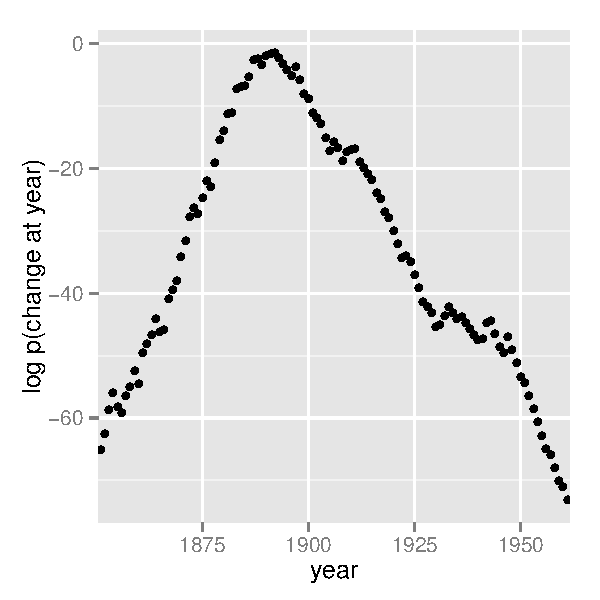
\includegraphics[height=2in]{img/change-point-posterior.pdf}
\ \ \ \ \
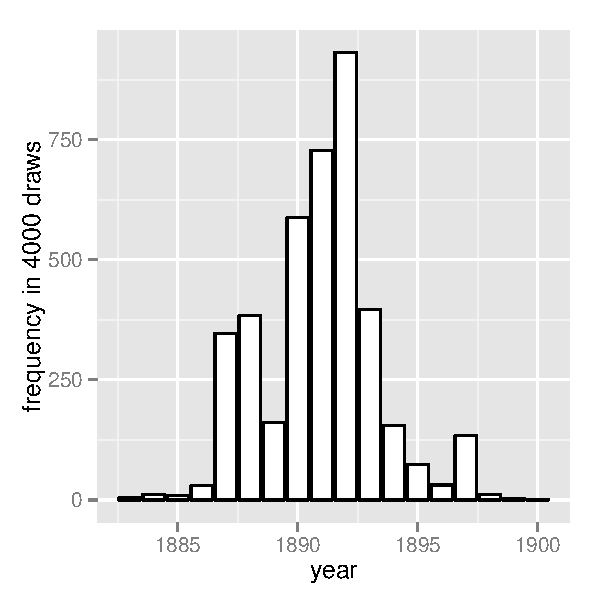
\includegraphics[height=2in]{img/s-discrete-posterior.pdf}
\end{center}
\vspace*{-12pt}
\caption{\small\it The posterior estimates for the change point.  \
  {\rm Left)} log probability of change point being in year,
  calculated analytically using \code{lp}; \ {\rm Right)}\ frequency
  of change point draws in the posterior generated using
  \code{lp}. The plot on the left is on the log scale and the plot on
  the right on the linear scale; note the narrower range of years in
  the right-hand plot resulting from sampling. The posterior mean of
  $s$ is roughly 1891.}%
\label{change-point-posterior.figure}
\end{figure}
%



\subsection{Discrete Sampling}

The generated quantities block may be used to draw discrete parameter
values using the built-in pseudo-random number generators.  For
example, with \code{lp} defined as above, the following program
draws a random value for \code{s} at every iteration.
%
\begin{stancode}
generated quantities {
  int<lower=1,upper=T> s;
  s = categorical_logit_rng(lp);
}
\end{stancode}
%
A posterior histogram of draws for $s$ is shown on the right side of
\reffigure{change-point-posterior}.

Compared to working in terms of expectations, discrete sampling is
highly inefficient, especially for tails of distributions, so this
approach should only be used if draws from a distribution are
explicitly required.   Otherwise, expectations should be computed in
the generated quantities block based on the posterior distribution for
\code{s} given by \code{softmax(lp)}.


\subsection{Posterior Covariance}

The discrete sample generated for $s$ can be used to calculate
covariance with other parameters.  Although the sampling approach is
straightforward, it is more statistically efficient (in the sense of
requiring far fewer iterations for the same degree of accuracy) to
calculate these covariances in expectation using \code{lp}.


\subsection{Multiple Change Points}

There is no obstacle in principle to allowing multiple change points.
The only issue is that computation increases from linear to quadratic
in marginalizing out two change points, cubic for three change points,
and so on.  There are three parameters, \code{e}, \code{m}, and
\code{l}, and two loops for the change point and then one over time,
with log densities being stored in a matrix.
%
\begin{stancode}
matrix[T, T] lp;
lp = rep_matrix(log_unif, T);
for (s1 in 1:T)
  for (s2 in 1:T)
    for (t in 1:T)
      lp[s1,s2] = lp[s1,s2]
        + poisson_lpmf(D[t] | t < s1 ? e : (t < s2 ? m : l));
\end{stancode}
%
The matrix can then be converted back to a vector using
\code{to\_vector} before being passed to \code{log\_sum\_exp}.

\section{Mark-Recapture Models}

A widely applied field method in ecology is to capture (or sight)
animals, mark them (e.g., by tagging), then release them.  This
process is then repeated one or more times, and is often done for
populations on an ongoing basis.  The resulting data may be used to
estimate population size.

The first subsection describes a very simple mark-recapture model that does
not involve any latent discrete parameters.  The following subsections
describes the Cormack-Jolly-Seber model, which involves latent
discrete parameters for animal death.

\subsection{Simple Mark-Recapture Model}

In the simplest case, a one-stage mark-recapture study produces the
following data
%
\begin{itemize}
\item $M$ : number of animals marked in first capture,
\item $C$ : number animals in second capture, and
\item $R$ : number of marked animals in second capture.
\end{itemize}
%
The estimand of interest is
%
\begin{itemize}
\item $N$ : number of animals in the population.
\end{itemize}
%
Despite the notation, the model will take $N$ to be a continuous
parameter; just because the population must be finite doesn't mean the
parameter representing it must be.  The parameter will be used to
produce a real-valued estimate of the population size.

The Lincoln-Petersen \citep{Lincoln:1930,Petersen:1896} method for
estimating population size is
%
\[
\hat{N} = \frac{M C}{R}.
\]
%
This population estimate would arise from a probabilistic model in
which the number of recaptured animals is distributed binomially,
\[
R \sim \distro{Binomial}(C, M / N)
\]
given the total number of animals captured in the second round ($C$)
with a recapture probability of $M/N$, the fraction of the total
population $N$ marked in the first round.

%
\begin{figure}
\begin{stancode}
data {
  int<lower=0> M;
  int<lower=0> C;
  int<lower=0,upper=min(M,C)> R;
}
parameters {
  real<lower=(C - R + M)> N;
}
model {
  R ~ binomial(C, M / N);
}
\end{stancode}
\vspace*{-6pt}
\caption{\small\it A probabilistic formulation of the Lincoln-Petersen
estimator for population size based on data from a one-step
mark-recapture study.  The lower bound on $N$ is necessary to
efficiently eliminate impossible values.}%
\label{lincoln-petersen-model.figure}
\end{figure}
%
The probabilistic variant of the Lincoln-Petersen estimator can be
directly coded in Stan as shown in \reffigure{lincoln-petersen-model}.
The Lincoln-Petersen estimate is the maximum likelihood estimate (MLE)
for this model.

To ensure the MLE is the Lincoln-Petersen estimate, an improper
uniform prior for $N$ is used; this could (and should) be replaced
with a more informative prior if possible based on knowledge of the
population under study.

The one tricky part of the model is the lower bound $C - R + M$ placed
on the population size $N$.  Values below this bound are impossible
because it is otherwise not possible to draw $R$ samples out of the
$C$ animals recaptured.  Implementing this lower bound is necessary to
ensure sampling and optimization can be carried out in an
unconstrained manner with unbounded support for parameters on the
transformed (unconstrained) space.  The lower bound in the declaration
for $C$ implies a variable transform $f : (C-R+M,\infty) \rightarrow
(-\infty,+\infty)$ defined by $f(N) = \log(N - (C - R + M))$; see
\refsection{lower-bound-transform} for more information on the
transform used for variables declared with a lower bound.

\subsection{Cormack-Jolly-Seber with Discrete Parameter}

The Cormack-Jolly-Seber (CJS) model
\citep{Cormack:1964,Jolly:1965,Seber:1965} is an open-population model
in which the population may change over time due to death; the
presentation here draws heavily on \citep{Schofield:2007}.

The basic data is
%
\begin{itemize}
\item $I$ : number of individuals,
\item $T$ : number of capture periods, and
\item $y_{i,t}$ : boolean indicating if individual $i$ was captured at
  time $t$.
\end{itemize}
%
Each individual is assumed to have been captured at least once because
an individual only contributes information conditionally after they
have been captured the first time.

There are two Bernoulli parameters in the model,
%
\begin{itemize}
\item $\phi_t$ : probability that animal alive at time $t$ survives
  until $t + 1$ and
\item $p_t$ : probability that animal alive at time $t$ is captured at
  time $t$.
\end{itemize}
%
These parameters will both be given uniform priors, but information
should be used to tighten these priors in practice.

The CJS model also employs a latent discrete parameter $z_{i,t}$
indicating for each individual $i$ whether it is alive at time $t$,
distributed as
%
\[
z_{i,t} \sim \distro{Bernoulli}(\ternary{z_{i,t-1}}{0}{\phi_{t-1}}).
\]
%
The conditional prevents the model positing zombies; once an animal is
dead, it stays dead.  The data distribution is then simple to express
conditional on $z$ as
%
\[
y_{i,t} \sim \distro{Bernoulli}(\ternary{z_{i,t}}{0}{p_t})
\]
%
The conditional enforces the constraint that dead animals cannot be captured.


\subsection{Collective Cormack-Jolly-Seber Model}

This subsection presents an implementation of the model in terms of
counts for different history profiles for individuals over three
capture times. It assumes exchangeability of the animals in that each
is assigned the same capture and survival probabilities.

In order to ease the marginalization of the latent discrete parameter
$z_{i,t}$, the Stan models rely on a derived quantity $\chi_t$ for
the probability that an individual is never captured again if it is
alive at time $t$ (if it is dead, the recapture probability is zero).
this quantity is defined recursively by
\[
\chi_t
=
\begin{cases}
1
& \mbox{if } t = T
\\[3pt]
(1 - \phi_t) + \phi_t (1 - p_{t+1}) \chi_{t+1}
& \mbox{ if } t < T
\end{cases}
\]
%
The base case arises because if an animal was captured in the last
time period, the probability it is never captured again is 1 because
there are no more capture periods.  The recursive case defining
$\chi_{t}$ in terms of $\chi_{t+1}$ involves two possibilities: (1)
not surviving to the next time period, with probability $(1 -
\phi_t)$, or (2) surviving to the next time period with probability
$\phi_t$, not being captured in the next time period with probability
$(1 - p_{t+1})$, and not being captured again after being alive in
period $t+1$ with probability $\chi_{t+1}$.

With three capture times, there are three captured/not-captured
profiles an individual may have.  These may be naturally coded as
binary numbers as follows.
%
\begin{center}
\begin{tabular}{c|ccc|c}
& \multicolumn{3}{|c|}{{\it captures}}
\\
{\it profile} & 1 & 2 & 3 & {\it probability}
\\ \hline
{0} & - & - & - & n/a
\\
{1} & - & - & + & n/a
\\ \hline
{2} & - & + & - & $\chi_2$
\\
{3} & - & + & + & $\phi_2 \, \phi_3$
\\ \hline
{4} & + & - & - & $\chi_1$
\\
{5} & + & - & + & $\phi_1 \, (1 - p_2) \, \phi_2 \, p_3$
\\ \hline
{6} & + & + & - & $ \phi_1 \, p_2 \, \chi_2$
\\
{7} & + & + & + & $\phi_1 \, p_2 \, \phi_2 \, p_3$
\end{tabular}
\end{center}
%
History 0, for animals that are never captured, is unobservable
because only animals that are captured are observed. History 1, for
animals that are only captured in the last round, provides no
information for the CJS model, because capture/non-capture status is
only informative when conditioned on earlier captures.  For the
remaining cases, the contribution to the likelihood is provided in the
final column.

By defining these probabilities in terms of $\chi$ directly, there is
no need for a latent binary parameter indicating whether an animal is
alive at time $t$ or not.  The definition of $\chi$ is typically used
to define the likelihood (i.e., marginalize out the latent discrete
parameter) for the CJS model \citep[page 9]{Schofield:2007}.

The Stan model defines $\chi$ as a transformed parameter based on
parameters $\phi$ and $p$.  In the model block, the log probability is
incremented for each history based on its count.  This second step is
similar to collecting Bernoulli observations into a binomial or
categorical observations into a multinomial, only it is coded directly
in the Stan program using \code{target~+=} rather than
being part of a built-in probability function.
%
\begin{figure}
\begin{stancode}
data {
  int<lower=0> history[7];
}
parameters {
  real<lower=0,upper=1> phi[2];
  real<lower=0,upper=1> p[3];
}
transformed parameters {
  real<lower=0,upper=1> chi[2];
  chi[2] = (1 - phi[2]) + phi[2] * (1 - p[3]);
  chi[1] = (1 - phi[1]) + phi[1] * (1 - p[2]) * chi[2];
}
model {
  target += history[2] * log(chi[2]);
  target += history[3] * (log(phi[2]) + log(p[3]));
  target += history[4] * (log(chi[1]));
  target += history[5] * (log(phi[1]) + log1m(p[2])
                            + log(phi[2]) + log(p[3]));
  target += history[6] * (log(phi[1]) + log(p[2])
                            + log(chi[2]));
  target += history[7] * (log(phi[1]) + log(p[2])
                            + log(phi[2]) + log(p[3]));
}
generated quantities {
  real<lower=0,upper=1> beta3;
  beta3 = phi[2] * p[3];
}
\end{stancode}
\vspace*{-12pt}
\caption{\small\it A Stan program for the Cormack-Jolly-Seber
  mark-recapture model that considers counts of individuals with
  observation histories of being observed or not in three capture
  periods.}\label{cjs-history.figure}
\end{figure}
%

\subsubsection{Identifiability}

The parameters $\phi_2$ and $p_3$, the probability of death at time 2
and probability of capture at time 3 are not identifiable, because both
may be used to account for lack of capture at time 3.  Their product,
$\beta_3 = \phi_2 \, p_3$, is identified.  The Stan model defines
\code{beta3} as a generated quantity.  Unidentified parameters pose a
problem for Stan's samplers' adaptation.  Although the problem posed
for adaptation is mild here because the parameters are bounded and
thus have proper uniform priors, it would be better to formulate an
identified parameterization.  One way to do this would be to formulate
a hierarchical model for the $p$ and $\phi$ parameters.

\subsection{Individual Cormack-Jolly-Seber Model}

This section presents a version of the Cormack-Jolly-Seber (CJS) model
cast at the individual level rather than collectively as in the
previous subsection.  It also extends the model to allow an arbitrary
number of time periods.  The data will consist of the number $T$ of
capture events, the number $I$ of individuals, and a boolean flag
$y_{i,t}$ indicating if individual $i$ was observed at time $t$.  In
Stan,
%
\begin{stancode}
data {
  int<lower=2> T;
  int<lower=0> I;
  int<lower=0,upper=1> y[I, T];
}
\end{stancode}

The advantages to the individual-level model is that it becomes
possible to add individual ``random effects'' that affect survival or
capture probability, as well as to avoid the combinatorics involved in
unfolding $2^T$ observation histories for $T$ capture times.

\subsubsection{Utility Functions}

The individual CJS model is written involves several function
definitions.  The first two are used in the transformed data block to
compute the first and last time period in which an animal was
captured.%
%
\footnote{An alternative would be to compute this on the outside and
feed it into the Stan model as preprocessed data.  Yet another
alternative encoding would be a sparse one recording only the
capture events along with their time and identifying the individual
captured.}
%
\begin{stancode}
functions {
  int first_capture(int[] y_i) {
    for (k in 1:size(y_i))
      if (y_i[k])
        return k;
    return 0;
  }
  int last_capture(int[] y_i) {
    for (k_rev in 0:(size(y_i) - 1)) {
      int k;
      k = size(y_i) - k_rev;
      if (y_i[k])
        return k;
    }
    return 0;
  }
  ...
}
\end{stancode}
%
These two functions are used to define the first and last capture time
for each individual in the transformed data block.%
%
\footnote{Both functions return 0 if the individual represented by the
  input array was never captured.  Individuals with no captures are
  not relevant for estimating the model because all probability
  statements are conditional on earlier captures.  Typically they
  would be removed from the data, but the program allows them to be
  included even though they make not contribution to the log
  probability function.}
%
\begin{stancode}
transformed data {
  int<lower=0,upper=T> first[I];
  int<lower=0,upper=T> last[I];
  vector<lower=0,upper=I>[T] n_captured;
  for (i in 1:I)
    first[i] = first_capture(y[i]);
  for (i in 1:I)
    last[i] = last_capture(y[i]);
  n_captured = rep_vector(0, T);
  for (t in 1:T)
    for (i in 1:I)
      if (y[i, t])
        n_captured[t] = n_captured[t] + 1;
}
\end{stancode}
%
The transformed data block also defines \code{n\_captured[t]}, which is
the total number of captures at time \code{t}.  The variable
\code{n\_captured} is defined as a vector instead of an integer array
so that it can be used in an elementwise vector operation in the generated
quantities block to model the population estimates at each time point.

The parameters and transformed parameters are as before, but now there
is a function definition for computing the entire vector \code{chi}, the
probability that if an individual is alive at \code{t} that it will
never be captured again.
%
\begin{stancode}
parameters {
  vector<lower=0,upper=1>[T-1] phi;
  vector<lower=0,upper=1>[T] p;
}
transformed parameters {
  vector<lower=0,upper=1>[T] chi;
  chi = prob_uncaptured(T,p,phi);
}
\end{stancode}
%
The definition of \code{prob\_uncaptured}, from the functions block,
is
%
\begin{stancode}
functions {
  ...
  vector prob_uncaptured(int T, vector p, vector phi) {
    vector[T] chi;
    chi[T] = 1.0;
    for (t in 1:(T - 1)) {
      int t_curr;
      int t_next;
      t_curr = T - t;
      t_next = t_curr + 1;
      chi[t_curr] = (1 - phi[t_curr])
                     + phi[t_curr]
                       * (1 - p[t_next])
                       * chi[t_next];
    }
    return chi;
  }
}
\end{stancode}
%
The function definition directly follows the mathematical definition
of $\chi_t$, unrolling the recursion into an iteration and
defining the elements of \code{chi} from \code{T} down to 1.

\subsubsection{The Model}

Given the precomputed quantities, the model block directly encodes the
CJS model's log likelihood function.  All parameters are left with
their default uniform priors and the model simply encodes the log
probability of the observations \code{q} given the parameters \code{p}
and \code{phi} as well as the transformed parameter \code{chi} defined
in terms of \code{p} and \code{phi}.
%
\begin{stancode}
model {
  for (i in 1:I) {
    if (first[i] > 0) {
      for (t in (first[i]+1):last[i]) {
        1 ~ bernoulli(phi[t-1]);
        y[i, t] ~ bernoulli(p[t]);
      }
      1 ~ bernoulli(chi[last[i]]);
    }
  }
}
\end{stancode}
%
The outer loop is over individuals, conditional skipping individuals
\code{i} which are never captured.  The never-captured check depends
on the convention of the first-capture and last-capture functions
returning 0 for \code{first} if an individual is never captured.

The inner loop for individual \code{i} first increments the log
probability based on the survival of the individual with probability
\code{phi[t-1]}.  The outcome of 1 is fixed because the individual
must survive between the first and last capture (i.e., no zombies).
Note that the loop starts after the first capture, because all
information in the CJS model is conditional on the first capture.

In the inner loop, the observed capture status \code{y[i,~t]} for
individual \code{i} at time \code{t} has a Bernoulli distribution
based on the capture probability \code{p[t]} at time \code{t}.

After the inner loop, the probability of an animal never being seen
again after being observed at time \code{last[i]} is included, because
\code{last[i]} was defined to be the last time period in which animal
\code{i} was observed.

\subsubsection{Identified Parameters}

As with the collective model described in the previous subsection,
this model does not identify \code{phi[T-1]} and \code{p[T]}, but
does identify their product, \code{beta}.  Thus \code{beta} is defined
as a generated quantity to monitor convergence and report.
%
\begin{stancode}
generated quantities {
  real beta;
  ...

  beta = phi[T-1] * p[T];
  ...
}
\end{stancode}
%

The parameter \code{p[1]} is also not modeled and will just be uniform
between 0 and 1.  A more finely articulated model might have a
hierarchical or time-series component, in which case \code{p[1]} would
be an unknown initial condition and both \code{phi[T-1]} and
\code{p[T]} could be identified.

\subsubsection{Population Size Estimates}

The generated quantities also calculates an estimate of the population
mean at each time \code{t} in the same way as in the simple
mark-recapture model as the number of individuals captured at time
\code{t} divided by the probability of capture at time \code{t}.  This
is done with the elementwise division operation for vectors
(\code{./}) in the generated quantities block.
%
\begin{stancode}
generated quantities {
  ...
  vector<lower=0>[T] pop;
  ...
  pop = n_captured ./ p;
  pop[1] = -1;
}
\end{stancode}

\subsubsection{Generalizing to Individual Effects}

All individuals are modeled as having the same capture probability,
but this model could be easily generalized to use a logistic
regression here based on individual-level inputs to be used as
predictors.



\section{Data Coding and Diagnostic Accuracy Models}

Although seemingly disparate tasks, the rating/coding/annotation of
items with categories and diagnostic testing for disease or other
conditions share several characteristics which allow their statistical
properties to modeled similarly.

\subsection{Diagnostic Accuracy}

Suppose you have diagnostic tests for a condition of varying
sensitivity and specificity.  Sensitivity is the probability a test
returns positive when the patient has the condition and specificity is
the probability that a test returns negative when the patient does not
have the condition.  For example, mammograms and puncture biopsy tests
both test for the presence of breast cancer.  Mammograms have high
sensitivity and low specificity, meaning lots of false positives,
whereas puncture biopsies are the opposite, with low sensitivity and
high specificity, meaning lots of false negatives.

There are several estimands of interest in such studies.  An
epidemiological study may be interested in the prevalence of a kind of
infection, such as malaria, in a population.  A test development study
might be interested in the diagnostic accuracy of a new test. A health
care worker performing tests might be interested in the disease status
of a particular patient.

\subsection{Data Coding}

Humans are often given the task of coding (equivalently rating or
annotating) data.  For example, journal or grant reviewers rate
submissions, a political study may code campaign commercials as to
whether they are attack ads or not, a natural language processing
study might annotate Tweets as to whether they are positive or
negative in overall sentiment, or a dentist looking at an X-ray
classifies a patient as having a cavity or not.  In all of these
cases, the data coders play the role of the diagnostic tests and all
of the same estimands are in play --- data coder accuracy and bias,
true categories of items being coded, or the prevalence of various
categories of items in the data.

\subsection{Noisy Categorical Measurement Model}

In this section, only categorical ratings are considered, and the
challenge in the modeling for Stan is to marginalize out the discrete
parameters.

\cite{DawidSkene:1979} introduce a noisy-measurement model for
data coding and apply in the epidemiological setting of coding what
doctor notes say about patient histories;  the same model can be used
for diagnostic procedures.

\subsubsection{Data}

The data for the model consists of $J$ raters (diagnostic tests), $I$
items (patients), and $K$ categories (condition statuses) to annotate,
with $y_{i, j} \in 1{:}K$ being the rating provided by rater $j$ for
item $i$.  In a diagnostic test setting for a particular condition,
the raters are diagnostic procedures and often $K=2$, with values
signaling the presence or absence of the condition.%
%
\footnote{Diagnostic procedures are often ordinal, as in stages of
  cancer in oncological diagnosis or the severity of a cavity in
  dental diagnosis.  Dawid and Skene's model may be used as is or
  naturally generalized for ordinal ratings using a latent continuous
  rating and cutpoints as in ordinal logistic regression.}

It is relatively straightforward to extend Dawid and Skene's model to
deal with the situation where not every rater rates each item exactly
once.

\subsection{Model Parameters}

The model is based on three parameters, the first of which is discrete:
%
\begin{itemize}
\item $z_i$ : a value in $1{:}K$ indicating the true category of item $i$,
\item $\pi$ : a $K$-simplex for the prevalence of the $K$
  categories in the population, and
\item $\theta_{j,k}$ : a $K$-simplex for the response of annotator $j$
  to an item of true category $k$.
\end{itemize}

\subsection{Noisy Measurement Model}

The true category of an item is assumed to be generated by a simple
categorical distribution based on item prevalence,
\[
z_i \sim \distro{Categorical}(\pi).
\]
%
The rating $y_{i, j}$ provided for item $i$ by rater $j$ is modeled as
a categorical response of rater $i$ to an item of category $z_i$,%
%
\footnote{In the subscript, $z[i]$ is written as $z_i$ to
  improve legibility.}
%
\[
y_{i, j} \sim \distro{Categorical}(\theta_{j,\pi_{z[i]}}).
\]

\subsubsection{Priors and Hierarchical Modeling}

Dawid and Skene provided maximum likelihood estimates for $\theta$ and
$\pi$, which allows them to generate probability estimates for each $z_i$.

To mimic Dawid and Skene's maximum likelihood model, the parameters
$\theta_{j,k}$ and $\pi$ can be given uniform priors over
$K$-simplexes.  It is straightforward to generalize to Dirichlet
priors,
\[
\pi \sim \distro{Dirichlet}(\alpha)
\]
and
\[
\theta_{j,k} \sim \distro{Dirichlet}(\beta_k)
\]
with fixed hyperparameters $\alpha$ (a vector) and $\beta$ (a matrix
or array of vectors).  The prior for $\theta_{j,k}$ must be allowed to
vary in $k$, so that, for instance, $\beta_{k,k}$ is large enough to
allow the prior to favor better-than-chance annotators over random or
adversarial ones.

Because there are $J$ coders, it would be natural to extend the model
to include a hierarchical prior for $\beta$ and to partially pool the
estimates of coder accuracy and bias.

\subsubsection{Marginalizing out the True Category}

Because the true category parameter $z$ is discrete, it must be
marginalized out of the joint posterior in order to carry out sampling
or maximum likelihood estimation in Stan. The joint posterior factors
as
\[
p(y, \theta, \pi) = p(y | \theta,\pi) \, p(\pi) \, p(\theta),
\]
where $p(y | \theta,\pi)$ is derived by marginalizing $z$ out of
%
\[
p(z, y | \theta, \pi)
\ = \
\prod_{i=1}^I \left( \distro{Categorical}(z_i | \pi)
                     \prod_{j=1}^J
                     \distro{Categorical}(y_{i, j}|\theta_{j, z[i]})
              \right).
\]
%
This can be done item by item, with
\[
p(y | \theta, \pi)
\ = \
\prod_{i=1}^I \sum_{k=1}^K
  \left( \distro{Categorical}(z_i | \pi)
         \prod_{j=1}^J
         \distro{Categorical}(y_{i, j}|\theta_{j, z[i]})
  \right).
\]
%
In the missing data model, only the observed labels would be used in
the inner product.

\cite{DawidSkene:1979} derive exactly the same equation in their
Equation~(2.7), required for the E-step in their expectation
maximization (EM) algorithm.  Stan requires the marginalized
probability function on the log scale,
\[
\begin{array}{l}
\mbox{ } \ \log p(y | \theta, \pi)
\\[3pt]
\mbox{ } \  = \
\sum_{i=1}^I \log \left( \sum_{k=1}^K \exp
  \left( \log \distro{Categorical}(z_i | \pi)
         + \sum_{j=1}^J
         \log \distro{Categorical}(y_{i, j}|\theta_{j, z[i]})
  \right) \right),
\end{array}
\]
which can be directly coded using Stan's built-in \code{log\_sum\_exp}
function.


\subsection{Stan Implementation}

The Stan program for the Dawid and Skene model is provided in
\reffigure{dawid-skene-model}.
%
\begin{figure}
\begin{stancode}
data {
  int<lower=2> K;
  int<lower=1> I;
  int<lower=1> J;

  int<lower=1,upper=K> y[I, J];

  vector<lower=0>[K] alpha;
  vector<lower=0>[K] beta[K];
}
parameters {
  simplex[K] pi;
  simplex[K] theta[J, K];
}
transformed parameters {
  vector[K] log_q_z[I];
  for (i in 1:I) {
    log_q_z[i] = log(pi);
    for (j in 1:J)
      for (k in 1:K)
        log_q_z[i, k] = log_q_z[i, k]
                         + log(theta[j, k, y[i, j]]);
  }
}
model {
  pi ~ dirichlet(alpha);
  for (j in 1:J)
    for (k in 1:K)
      theta[j, k] ~ dirichlet(beta[k]);

  for (i in 1:I)
    target += log_sum_exp(log_q_z[i]);
}
\end{stancode}
\vspace*{-12pt}
\caption{\small\it Stan program for the rating (or diagnostic
  accuracy) model of \cite{DawidSkene:1979}. The model marginalizes
  out the discrete parameter $z$, storing the unnormalized conditional
  probability $\log q(z_i=k|\theta,\pi)$ in\ \code{log\_q\_z[i,~k]}.}%
\label{dawid-skene-model.figure}
\end{figure}
%
The Stan model converges quickly and mixes well using NUTS starting at
diffuse initial points, unlike the equivalent model implemented with
Gibbs sampling over the discrete parameter.  Reasonable weakly
informative priors are $\alpha_k = 3$ and $\beta_{k,k} = 2.5 K$ and
$\beta_{k,k'} = 1$ if $k \neq k'$.  Taking $\alpha$ and $\beta_k$ to
be unit vectors and applying optimization will produce the same answer
as the expectation maximization (EM) algorithm of
\cite{DawidSkene:1979}.

\subsubsection{Inference for the True Category}

The quantity \code{log\_q\_z[i]} is defined as a transformed
parameter.  It encodes the (unnormalized) log of $p(z_i | \theta,
\pi)$.  Each iteration provides a value conditioned on that
iteration's values for $\theta$ and $\pi$.  Applying the softmax
function to \code{log\_q\_z[i]} provides a simplex corresponding to
the probability mass function of $z_i$ in the posterior.   These may
be averaged across the iterations to provide the posterior probability
distribution over each $z_i$.


\chapter{Sparse and Ragged Data Structures}\label{sparse-ragged.chapter}

\noindent
Stan does not directly support either sparse or ragged data
structures, though both can be accommodated with some programming
effort.  \refchapter{sparse-matrices} introduces a special-purpose
sparse matrix times dense vector multiplication, which should be used
where applicable;  this chapter covers more general data structures.

\section{Sparse Data Structures}

Coding sparse data structures is as easy as moving from a matrix-like
data structure to a database-like data structure.  For example,
consider the coding of sparse data for the IRT models discussed in
\refsection{item-response-models}.  There are $J$ students and $K$
questions, and if every student answers every question, then it is
practical to declare the data as a $J \times K$ array of answers.
%
\begin{quote}
\begin{Verbatim}
data {
  int<lower=1> J;
  int<lower=1> K;
  int<lower=0,upper=1> y[J, K];
  ...
model {
  for (j in 1:J)
    for (k in 1:K)
      y[j, k] ~ bernoulli_logit(delta[k] * (alpha[j] - beta[k]));
  ...
\end{Verbatim}
\end{quote}
%

\begin{figure}
\begin{center}
\begin{minipage}[c]{0.45\textwidth}
\[
y
=
\left[
\begin{array}{cccc}
0 & 1 & \mbox{NA} & 1
\\
0 & \mbox{NA} & \mbox{NA} & 1
\\
\mbox{NA} & 0 & \mbox{NA} & \mbox{NA}
\end{array}
\right]
\]
\end{minipage}
\ \ \
\begin{minipage}[c]{0.45\textwidth}
\begin{tabular}{ll|l}
$jj$ & $kk$ & $y$
\\ \hline
1 & 1 & 0
\\
1 & 2 & 1
\\
1 & 4 & 1
\\
2 & 1 & 0
\\
2 & 4 & 1
\\
3 & 2 & 0
\end{tabular}
\end{minipage}
\end{center}
\vspace*{-12pt}
\caption{\small\it  Example of coding sparse arrays in Stan.  On the left is a definition
  of a sparse matrix $y$ using the NA notation from R (which is not
  supported by Stan).  On the right is a database-like encoding of the
  same sparse matrix $y$ that can be used directly in Stan.  The first
  two columns, $jj$ and $kk$, denote the indexes and the final column,
  $y$, the value.  For example, the fifth row of the database-like
  data structure on the right indicates that $y_{2,4} = 1$.}\label{sparse-data.figure}
\end{figure}
%
When not every student is given every question, the dense array coding
will no longer work, because Stan does not support undefined values.
\reffigure{sparse-data} shows an example with $J=3$ and $K=4$, with
missing responses shown as NA, as in R.  There is no support within
Stan for R's NA values, so this data structure cannot be used
directly.  Instead, it must be converted to a ``long form'' as in a
database, with columns indicating the $j$ and $k$ indexes along with
the value.  For instance, with $jj$ and $kk$ used for the indexes
(following \citep{GelmanHill:2007}), the data structure can be coded
as in the right-hand example in \reffigure{sparse-data}.  This says
that $y_{1,1} = 0$, $y_{1,2} = 1$, and so on, up to $y_{3,2} = 1$,
with all other entries undefined.

Letting $N$ be the number of $y$ that are defined, here $N=6$,
the data and model can be formulated as follows.
%
\begin{quote}
\begin{Verbatim}
data {
  ...
  int<lower=1> N;
  int<lower=1,upper=J> jj[N];
  int<lower=1,upper=K> kk[N];
  int<lower=0,upper=1> y[N];
  ...
model {
  for (n in 1:N)
    y[n] ~ bernoulli_logit(delta[kk[n]]
                           * (alpha[jj[n]] - beta[kk[n]]));
  ...
\end{Verbatim}
\end{quote}
%
In the situation where there are no missing values, the two model
formulations produce exactly the same log posterior density.


\section{Ragged Data Structures}\label{ragged-data-structs.section}

Ragged arrays are arrays that are not rectangular, but have different
sized entries.  This kind of structure crops up when there are
different numbers of observations per entry.

A general approach to dealing with ragged structure is to move to a
full database-like data structure as discussed in the previous
section.  A more compact approach is possible with some indexing into
a linear array.

For example, consider a data structure for three groups, each of which
has a different number of observations.
%
\begin{figure}
\begin{center}
\begin{minipage}[c]{0.35\textwidth}
$y_1 =  \left[1.3 \ \ 2.4 \ \ 0.9\right]$
\\[3pt]
$y_2 = \left[-1.8 \ \ -0.1\right]$
\\[3pt]
$y_3 = \left[12.9 \ \ 18.7 \ \ 42.9 \ \ 4.7\right]$
\end{minipage}
\ \ \
\begin{minipage}[c]{0.60\textwidth}
$z = [1.3 \ \ 2.4 \ \ 0.9 \ \ -1.8 \ \ -0.1 \ \ 12.9 \ \ 18.7 \ \ 42.9
\ \ 4.7]$
\\[3pt]
$s  =  \{ 3 \ \ 2 \ \ 4 \}$
\end{minipage}
\end{center}
\caption{\small\it Example of coding ragged arrays in Stan.  On the
  left is the definition of a ragged data structure $y$ with three
  rows of different sizes ($y_1$ is size 3, $y_2$ size 2, and $y_3$
  size 4).  On the right is an example of how to code the data in Stan,
  using a single vector $y$ to hold all the values and a separate
  array of integers $s$ to hold the group row sizes.  In this
  example, $y_1 = z_{1:3}$, $y_2 =
  z_{4:5}$, and $y_3 = z_{6:9}$.}\label{ragged-data.figure}
\end{figure}
%

Suppose the model is a very simple varying intercept model, which,
using vectorized notation, would yield a likelihood
\[
\prod_{n=1}^3 \log \distro{Normal}(y_n | \mu_n, \sigma).
\]
There's no direct way to encode this in Stan.

A full database type structure could be used, as in the sparse
example, but this is inefficient, wasting space for unnecessary
indices and not allowing vector-based density operations.  A better
way to code this data is as a single list of values, with a separate
data structure indicating the sizes of each subarray.  This is
indicated on the right of \reffigure{ragged-data}.  This coding uses a
single array for the values and a separate array for the sizes of each
row.

The model can then be coded up using slicing operations as follows.
\begin{quote}
\begin{Verbatim}
data {
  int<lower=0> N;   // # observations
  int<lower=0> K;   // # of groups
  vector[N] y;      // observations
  int s[K];         // group sizes
  ...
model {
  int pos;
  pos = 1;
  for (k in 1:K) {
    segment(y, pos, s[k]) ~ normal(mu[k], sigma);
    pos = pos + s[k];
  }
\end{Verbatim}
\end{quote}
%
This coding allows for efficient vectorization, which is worth the
copy cost entailed by the \code{segment()} vector slicing operation.


\chapter{Clustering Models}\label{clustering.chapter}

\noindent
Unsupervised methods for organizing data into groups are collectively
referred to as clustering.  This chapter describes the implementation
in Stan of two widely used statistical clustering models, soft
$K$-means and latent Dirichlet allocation (LDA).  In addition, this
chapter includes naive Bayesian classification, which can be viewed as
a form of clustering which may be supervised.  These models are
typically expressed using discrete parameters for cluster assignments.
Nevertheless, they can be implemented in Stan like any other mixture
model by marginalizing out the discrete parameters (see
\refchapter{mixture-modeling}).

\section{Relation to Finite Mixture Models}

As mentioned in \refsection{clustering-mixture}, clustering models and
finite mixture models are really just two sides of the same coin.  The
``soft'' $K$-means model described in the next section is a normal
mixture model (with varying assumptions about covariance in higher
dimensions leading to variants of $K$-means).  Latent Dirichlet
allocation is a mixed-membership multinomial mixture.

\section{Soft $K$-Means}

$K$-means clustering is a method of clustering data represented as
$D$-dimensional vectors.  Specifically, there will be $N$ items to be
clustered, each represented as a vector $y_n \in \reals^D$.  In the
``soft'' version of $K$-means, the assignments to clusters will be
probabilistic.

\subsection{Geometric Hard  $K$-Means Clustering}

$K$-means clustering is typically described geometrically in terms of
the following algorithm, which assumes the number of clusters $K$ and
data vectors $y$ as input.
%
\begin{enumerate}
\item For each $n$ in $1:N$, randomly assign vector $y_n$ to a cluster in $1{:}K$;
\item Repeat
\begin{enumerate}
\item For each cluster $k$ in $1{:}K$, compute the cluster centroid $\mu_k$  by averaging the
  vectors assigned to that cluster;
\item For each $n$ in $1:N$, reassign $y_n$ to the cluster $k$
  for which the (Euclidean) distance from $y_n$ to $\mu_k$ is smallest;
\item If no vectors changed cluster, return the cluster assignments.
\end{enumerate}
\end{enumerate}
%
This algorithm is guaranteed to terminate.

\subsection{Soft $K$-Means Clustering}

Soft $K$-means clustering treats the cluster assignments as
probability distributions over the clusters.  Because of the
connection between Euclidean distance and multivariate normal models
with a fixed covariance, soft $K$-means can be expressed (and coded in
Stan) as a multivariate normal mixture model.

In the full generative model, each data point $n$ in $1{:}N$ is assigned
a cluster $z_n \in 1{:}K$ with symmetric uniform probability,
%
\[
z_n \sim \distro{Categorical}({\bf 1}/K),
\]
where ${\bf 1}$ is the unit vector of $K$ dimensions, so that ${\bf
  1}/K$ is the symmetric $K$-simplex.  Thus the model assumes that
each data point is drawn from a hard decision about cluster
membership.  The softness arises only from the uncertainty about which
cluster generated a data point.

The data points themselves are generated from a multivariate normal
distribution whose parameters are determined by the cluster assignment
$z_n$,
\[
y_n \sim  \distro{Normal}(\mu_{z[n]},\Sigma_{z[n]})
\]

The sample implementation in this section assumes a fixed unit
covariance matrix shared by all clusters $k$,
\[
\Sigma_k = \mbox{diag\_matrix}({\bf 1}),
\]
so that the log multivariate normal can be implemented directly up to a proportion
by
\[
\mbox{Normal}\left( y_n | \mu_k, \mbox{diag\_matrix}({\bf 1}) \right)
\propto \exp \left (- \frac{1}{2} \sum_{d=1}^D \left( \mu_{k,d} - y_{n,d}
  \right)^2 \right).
\]
The spatial perspective on $K$-means arises by noting that the inner
term is just half the negative Euclidean distance from the cluster
mean $\mu_k$ to the data point $y_n$.

\subsection{Stan Implementation of Soft $K$-Means}

Consider the following Stan program for implementing $K$-means
clustering.%
%
\footnote{The model is available in the Stan example model repository;
see \url{http://mc-stan.org/documentation}.}
%
\begin{stancode}
data {
  int<lower=0> N;  // number of data points
  int<lower=1> D;  // number of dimensions
  int<lower=1> K;  // number of clusters
  vector[D] y[N];  // observations
}
transformed data {
  real<upper=0> neg_log_K;
  neg_log_K = -log(K);
}
parameters {
  vector[D] mu[K]; // cluster means
}
transformed parameters {
  real<upper=0> soft_z[N, K]; // log unnormalized clusters
  for (n in 1:N)
    for (k in 1:K)
      soft_z[n, k] = neg_log_K
                     - 0.5 * dot_self(mu[k] - y[n]);
}
model {
  // prior
  for (k in 1:K)
    mu[k] ~ normal(0, 1);

  // likelihood
  for (n in 1:N)
    target += log_sum_exp(soft_z[n]));
}
\end{stancode}
%
There is an independent unit normal prior on the centroid parameters;
this prior could be swapped with other priors, or even a hierarchical
model to fit an overall problem scale and location.

The only parameter is \code{mu}, where \code{mu[k]} is the centroid
for cluster $k$.  The transformed parameters \code{soft\_z[n]} contain
the log of the unnormalized cluster assignment probabilities.  The
vector \code{soft\_z[n]} can be converted back to a normalized simplex
using the softmax function (see \refsection{softmax}), either
externally or within the model's generated quantities block.

\subsection{Generalizing Soft $K$-Means}

The multivariate normal distribution with unit covariance matrix
produces a log probability density proportional to Euclidean distance
(i.e., $L_2$ distance).  Other distributions relate to other
geometries.  For instance, replacing the normal distribution with the
double exponential (Laplace) distribution produces a clustering model
based on $L_1$ distance (i.e., Manhattan or taxicab
distance).

Within the multivariate normal version of $K$-means, replacing the
unit covariance matrix with a shared covariance matrix amounts to
working with distances defined in a space transformed by the inverse
covariance matrix.

Although there is no global spatial analog, it is common to see soft
$K$-means specified with a per-cluster covariance matrix. In this
situation, a hierarchical prior may be used for the covariance matrices.



\section{The Difficulty of Bayesian Inference for Clustering}

Two problems make it pretty much impossible to perform full Bayesian
inference for clustering models, the lack of parameter identifiability
and the extreme multimodality of the posteriors.  There is additional
discussion related to the non-identifiability due to label switching
in \refsection{label-switching-problematic}.

\subsection{Non-Identifiability}

Cluster assignments are not identified --- permuting the cluster mean
vectors \code{mu} leads to a model with identical likelihoods.  For
instance, permuting the first two indexes in \code{mu} and the first
two indexes in each \code{soft\_z[n]} leads to an identical likelihood
(and prior).

The lack of identifiability means that the cluster parameters
cannot be compared across multiple Markov chains.  In fact, the only
parameter in soft $K$-means is not identified, leading to problems in
monitoring convergence.  Clusters can even fail to be identified
within a single chain, with indices swapping if the chain is long
enough or the data is not cleanly separated.

\subsection{Multimodality}

The other problem with clustering models is that their posteriors are
highly multimodal.  One form of multimodality is the
non-identifiability leading to index swapping.  But even without
the index problems the posteriors are highly multimodal.

Bayesian inference fails in cases of high multimodality because there
is no way to visit all of the modes in the posterior in appropriate
proportions and thus no way to evaluate integrals involved in
posterior predictive inference.

In light of these two problems, the advice often given in fitting
clustering models is to try many different initializations and select
the sample with the highest overall probability.  It is also popular
to use optimization-based point estimators such as expectation
maximization or variational Bayes, which can be much more efficient
than sampling-based approaches.


\section{Naive Bayes Classification and Clustering}

Naive Bayes is a kind of mixture model that can be used for
classification or for clustering (or a mix of both), depending on
which labels for items are observed.%
%
\footnote{For clustering, the non-identifiability problems for all
  mixture models present a problem, whereas there is no such problem
  for classification.  Despite the difficulties with full Bayesian
  inference for clustering, researchers continue to use it, often in
  an exploratory data analysis setting rather than for predictive
  modeling.}

Multinomial mixture models are referred to as ``naive Bayes'' because
they are often applied to classification problems where the
multinomial independence assumptions are clearly false.

Naive Bayes classification and clustering can be applied to any data
with multinomial structure.  A typical example of this is natural
language text classification and clustering, which is used an example
in what follows.

The observed data consists of a sequence of $M$ documents made up of
bags of words drawn from a vocabulary of $V$ distinct words.  A
document $m$ has $N_m$ words, which are indexed as $w_{m,1}, \ldots,
w_{m,N[m]} \in 1{:}V$.  Despite the ordered indexing of words in a
document, this order is not part of the model, which is clearly
defective for natural human language data.  A number of topics (or
categories) $K$ is fixed.

The multinomial mixture model generates a single category $z_m \in
1{:}K$ for each document $m \in 1{:}M$ according to a categorical
distribution,
\[
z_m \sim \distro{Categorical}(\theta).
\]
The $K$-simplex parameter $\theta$ represents the prevalence of each
category in the data.

Next, the words in each document are generated conditionally
independently of each other and the words in other documents based on
the category of the document, with word $n$ of document $m$ being
generated as
\[
w_{m,n} \sim \distro{Categorical}(\phi_{z[m]}).
\]
The parameter $\phi_{z[m]}$ is a $V$-simplex representing the
probability of each word in the vocabulary in documents of category
$z_m$.

The parameters $\theta$ and $\phi$ are typically given symmetric
Dirichlet priors.  The prevalence $\theta$ is sometimes fixed to
produce equal probabilities for each category $k \in 1:K$.

\subsection{Coding Ragged Arrays}

The specification for naive Bayes in the previous sections have used a ragged
array notation for the words $w$.  Because Stan does not support
ragged arrays, the models are coded using an alternative strategy that
provides an index for each word in a global list of words.   The data
is organized as follows, with the word arrays laid out in a column and each
assigned to its document in a second column.
%
\begin{center}
\begin{tabular}{r|cc}
\code{n} & \code{w[n]} & \code{doc[n]} \\ \hline
1 & $w_{1,1}$ & 1 \\
2 & $w_{1,2}$ & 1 \\
\vdots & \vdots & \vdots \\
$N_1$ & $w_{1,N[1]}$ & 1 \\
$N_1 + 1$ & $w_{2,1}$ & 2 \\
$N_1 + 2$ & $w_{2,2}$ & 2 \\
\vdots & \vdots & \vdots \\
$N_1 + N_2$ & $w_{2,N[2]}$ & 2 \\
$N_1 + N_2 + 1$ & $w_{3,1}$ & 3 \\
\vdots & \vdots & \vdots \\
$\code{N} = \sum_{m=1}^M N_m$ & $w_{M,N[M]}$ & $M$ \\
\end{tabular}
\end{center}
%
The relevant variables for the program are \code{N}, the total number
of words in all the documents, the word array \code{w}, and the
document identity array \code{doc}.

\subsection{Estimation with Category-Labeled Training Data}


A naive Bayes model for estimating the simplex parameters given
training data with documents of known categories can be coded in Stan
as follows%
%
\footnote{This model is available in the example model repository;
  see \url{http://mc-stan.org/documentation}.}
%
\begin{stancode}
data {
  // training data
  int<lower=1> K;               // num topics
  int<lower=1> V;               // num words
  int<lower=0> M;               // num docs
  int<lower=0> N;               // total word instances
  int<lower=1,upper=K> z[M];    // topic for doc m
  int<lower=1,upper=V> w[N];    // word n
  int<lower=1,upper=M> doc[N];  // doc ID for word n
  // hyperparameters
  vector<lower=0>[K] alpha;     // topic prior
  vector<lower=0>[V] beta;      // word prior
}
parameters {
  simplex[K] theta;   // topic prevalence
  simplex[V] phi[K];  // word dist for topic k
}
model {
  theta ~ dirichlet(alpha);
  for (k in 1:K)
    phi[k] ~ dirichlet(beta);
  for (m in 1:M)
    z[m] ~ categorical(theta);
  for (n in 1:N)
    w[n] ~ categorical(phi[z[doc[n]]]);
}
\end{stancode}
%
Note that the topic identifiers $z_m$ are declared as data and the
latent category assignments are included as part of the likelihood
function.

\subsection{Estimation without Category-Labeled Training Data}

Naive Bayes models can be used in an unsupervised fashion to cluster
multinomial-structured data into a fixed number $K$ of categories.
The data declaration includes the same variables as the model in the
previous section excluding the topic labels \code{z}.   Because
\code{z} is discrete, it needs to be summed out of the model
calculation.  This is done for naive Bayes as for other mixture
models.  The parameters are the same up to the priors, but the
likelihood is now computed as the marginal document probability
\[
\begin{array}{l}
\log p(w_{m,1},\ldots,w_{m,N_m}|\theta,\phi)
\\[2pt]
\ \ \ = \
\log \sum_{k=1}^K
\left( \distro{Categorical}(k|\theta)
        \times \prod_{n=1}^{N_m} \distro{Categorical}(w_{m,n}|\phi_k)
\right)
\\[6pt]
\ \ \ = \
\log \sum_{k=1}^K \exp \left(
\log \distro{Categorical}(k|\theta)
+ \sum_{n=1}^{N_m} \log \distro{Categorical}(w_{m,n}|\phi_k)
\right).
\end{array}
\]
%
The last step shows how the \code{log\_sum\_exp} function can be used
to stabilize the numerical calculation and return a result on the log
scale.
%
\begin{stancode}
model {
  real gamma[M, K];
  theta ~ dirichlet(alpha);
  for (k in 1:K)
    phi[k] ~ dirichlet(beta);
  for (m in 1:M)
    for (k in 1:K)
      gamma[m, k] = categorical_lpmf(k | theta);
  for (n in 1:N)
    for (k in 1:K)
      gamma[doc[n], k] = gamma[doc[n], k]
                         + categorical_lpmf(w[n] | phi[k]);
  for (m in 1:M)
    target += log_sum_exp(gamma[m]);
}
\end{stancode}
%
The local variable \code{gamma[m, k]} represents the value
\[
\gamma_{m,k} = \log \distro{Categorical}(k|\theta)
+ \sum_{n=1}^{N_m} \log \distro{Categorical}(w_{m,n}|\phi_k).
\]
%
Given $\gamma$, the posterior probability that document
$m$ is assigned category $k$ is
\[
\mbox{Pr}[z_m = k|w,\alpha,\beta]
=
\exp \left(
\gamma_{m,k}
- \log \sum_{k=1}^K \exp \left( \gamma_{m,k} \right)
\right).
\]
%
If the variable \code{gamma} were declared and defined in the
transformed parameter block, its sampled values would be saved by
Stan.  The normalized posterior probabilities could also be defined as
generated quantities.

\subsection{Full Bayesian Inference for Naive Bayes}

Full Bayesian posterior predictive inference for the naive Bayes model
can be implemented in Stan by combining the models for labeled and
unlabeled data.  The estimands include both the model parameters and
the posterior distribution over categories for the unlabeled data.  The
model is essentially a missing data model assuming the unknown
category labels are missing completely at random; see
\citep{GelmanEtAl:2013,GelmanHill:2007} for more
information on missing data imputation.  The model is also an instance
of semisupervised learning because the unlabeled data contributes to
the parameter estimations.

To specify a Stan model for performing full Bayesian inference, the
model for labeled data is combined with the model for unlabeled data.
A second document collection is declared as data, but without the
category labels, leading to new variables \code{M2} \code{N2},
\code{w2}, \and \code{doc2}.  The number of categories and number of
words, as well as the hyperparameters are shared and only declared
once.  Similarly, there is only one set of parameters.  Then the model
contains a single set of statements for the prior, a set of statements
for the labeled data, and a set of statements for the unlabeled data.

\subsection{Prediction without Model Updates}

An alternative to full Bayesian inference involves estimating a model
using labeled data, then applying it to unlabeled data without
updating the parameter estimates based on the unlabeled data.  This
behavior can be implemented by moving the definition of \code{gamma}
for the unlabeled documents to the generated quantities block.
Because the variables no longer contribute to the log probability,
they no longer jointly contribute to the estimation of the model
parameters.


\section{Latent Dirichlet Allocation}

Latent Dirichlet allocation (LDA) is a mixed-membership multinomial
clustering model \citep{BleiNgJordan:2003} that generalized naive
Bayes.  Using the topic and document terminology common in discussions of
LDA, each document is modeled as having a mixture of topics, with each
word drawn from a topic based on the mixing proportions.

\subsection{The LDA Model}

The basic model assumes each document is generated independently based
on fixed hyperparameters. For document $m$, the first step is to draw a topic
distribution simplex $\theta_m$ over the $K$ topics,
%
\[
\theta_m \sim \distro{Dirichlet}(\alpha).
\]
%
The prior hyperparameter $\alpha$ is fixed to a $K$-vector of positive
values.  Each word in the document is generated independently
conditional on the distribution $\theta_m$.  First, a topic
$z_{m,n} \in 1{:}K$ is drawn for the word based on the
document-specific topic-distribution,
\[
z_{m,n} \sim \distro{Categorical}(\theta_m).
\]
%
Finally, the word $w_{m,n}$ is drawn according to the word distribution
for topic $z_{m,n}$,
\[
w_{m,n} \sim \distro{Categorical}(\phi_{z[m,n]}).
\]
The distributions $\phi_k$ over words for topic $k$ are also given a
Dirichlet prior,
\[
\phi_k \sim \distro{Dirichlet}(\beta)
\]
%
where $\beta$ is a fixed $V$-vector of positive values.

\subsection{Summing out the Discrete Parameters}

Although Stan does not (yet) support discrete sampling, it is possible
to calculate the marginal distribution over the continuous parameters
by summing out the discrete parameters as in other mixture models.
The marginal posterior of the topic and word variables is
%
\begin{eqnarray*}
p(\theta,\phi|w,\alpha,\beta)
& \propto &
p(\theta|\alpha) \times p(\phi|\beta) \times p(w|\theta,\phi)
\\[4pt]
& = &
\prod_{m=1}^M p(\theta_m|\alpha)
\times
\prod_{k=1}^K p(\phi_k|\beta)
\times
\prod_{m=1}^M \prod_{n=1}^{M[n]} p(w_{m,n}|\theta_m,\phi).
\end{eqnarray*}
%
The inner word-probability term is defined by summing out the
topic assignments,
\begin{eqnarray*}
p(w_{m,n}|\theta_m,\phi)
& = &
\sum_{z=1}^K p(z,w_{m,n}|\theta_m,\phi).
\\[4pt]
& = &
\sum_{z=1}^K p(z|\theta_m) \times p(w_{m,n}|\phi_z).
\end{eqnarray*}
%
Plugging the distributions in and converting to the log scale provides a
formula that can be implemented directly in Stan,
\[
\begin{array}{l}
\log p(\theta,\phi|w,\alpha,\beta)
\\[6pt]
{ } \ \
\begin{array}{l}
{ } = \sum_{m=1}^M \log \distro{Dirichlet}(\theta_m|\alpha)
\ + \
\sum_{k=1}^K \log \distro{Dirichlet}(\phi_k|\beta)
\\[6pt]
{ } \ \ \ \ \
+ \sum_{m=1}^M \sum_{n=1}^{N[m]} \log \left(
\sum_{z=1}^K
  \distro{Categorical}(z|\theta_m)
   \times \distro{Categorical}(w_{m,n}|\phi_z)
 \right)
\end{array}
\end{array}
\]

\subsection{Implementation of LDA}


Applying the marginal derived in the last section to the data
structure described in this section leads to the following Stan
program for LDA.
%
\begin{stancode}
data {
  int<lower=2> K;               // num topics
  int<lower=2> V;               // num words
  int<lower=1> M;               // num docs
  int<lower=1> N;               // total word instances
  int<lower=1,upper=V> w[N];    // word n
  int<lower=1,upper=M> doc[N];  // doc ID for word n
  vector<lower=0>[K] alpha;     // topic prior
  vector<lower=0>[V] beta;      // word prior
}
parameters {
  simplex[K] theta[M];   // topic dist for doc m
  simplex[V] phi[K];     // word dist for topic k
}
model {
  for (m in 1:M)
    theta[m] ~ dirichlet(alpha);  // prior
  for (k in 1:K)
    phi[k] ~ dirichlet(beta);     // prior
  for (n in 1:N) {
    real gamma[K];
    for (k in 1:K)
      gamma[k] = log(theta[doc[n], k]) + log(phi[k, w[n]]);
    target += log_sum_exp(gamma);  // likelihood;
  }
}
\end{stancode}
%
As in the other mixture models, the log-sum-of-exponents function is
used to stabilize the numerical arithmetic.

\subsection{Correlated Topic Model}

To account for correlations in the distribution of topics for
documents, \citep{BleiLafferty:2007} introduced a variant of LDA in
which the Dirichlet prior on the per-document topic distribution is
replaced with a multivariate logistic normal distribution.

The authors treat the prior as a fixed hyperparameter.  They use an
$L_1$-regularized estimate of covariance, which is equivalent to the
maximum a posteriori estimate given a double-exponential prior.  Stan
does not (yet) support maximum a posteriori estimation, so the mean and
covariance of the multivariate logistic normal must be specified as
data.

\subsubsection{Fixed Hyperparameter Correlated Topic Model}

The Stan model in the previous section can be modified to implement
the correlated topic model by replacing the Dirichlet topic prior
\code{alpha} in the data declaration with the mean and covariance of
the multivariate logistic normal prior.
%
\begin{stancode}
data {
  ... data as before without alpha ...
  vector[K] mu;          // topic mean
  cov_matrix[K] Sigma;   // topic covariance
}
\end{stancode}
%
Rather than drawing the simplex parameter \code{theta} from a
Dirichlet, a parameter \code{eta} is drawn from a multivariate normal
distribution and then transformed using softmax into a simplex.
%
\begin{stancode}
parameters {
  simplex[V] phi[K];  // word dist for topic k
  vector[K] eta[M];   // topic dist for doc m
}
transformed parameters {
  simplex[K] theta[M];
  for (m in 1:M)
    theta[m] = softmax(eta[m]);
}
model {
  for (m in 1:M)
    eta[m] ~ multi_normal(mu, Sigma);
  ... model as before w/o prior for theta ...
}
\end{stancode}

\subsubsection{Full Bayes Correlated Topic Model}

By adding a prior for the mean and covariance, Stan supports full
Bayesian inference for the correlated topic model.  This requires
moving the declarations of topic mean \code{mu} and covariance \code{Sigma}
from the data block to the parameters block and providing them with
priors in the model.  A relatively efficient and interpretable prior
for the covariance matrix \code{Sigma} may be encoded as follows.
%
\begin{stancode}
... data block as before, but without alpha ...
parameters {
  vector[K] mu;              // topic mean
  corr_matrix[K] Omega;      // correlation matrix
  vector<lower=0>[K] sigma;  // scales
  vector[K] eta[M];          // logit topic dist for doc m
  simplex[V] phi[K];         // word dist for topic k
}
transformed parameters {
  ... eta as above ...
  cov_matrix[K] Sigma;       // covariance matrix
  for (m in 1:K)
    Sigma[m, m] = sigma[m] * sigma[m] * Omega[m, m];
  for (m in 1:(K-1)) {
    for (n in (m+1):K) {
      Sigma[m, n] = sigma[m] * sigma[n] * Omega[m, n];
      Sigma[n, m] = Sigma[m, n];
    }
  }
}
model {
  mu ~ normal(0, 5);      // vectorized, diffuse
  Omega ~ lkj_corr(2.0);  // regularize to unit correlation
  sigma ~ cauchy(0, 5);   // half-Cauchy due to constraint
  ... words sampled as above ...
}
\end{stancode}
%
The $\distro{LkjCorr}$ distribution with shape $\alpha > 0$ has support
on correlation matrices (i.e., symmetric positive definite with unit
diagonal).  Its density is defined by
\[
\distro{LkjCorr}(\Omega|\alpha) \propto \mbox{det}(\Omega)^{\alpha - 1}
\]
With a scale of $\alpha = 2$, the weakly informative prior favors a
unit correlation matrix.  Thus the compound effect of this prior on
the covariance matrix $\Sigma$ for the multivariate logistic normal is
a slight concentration around diagonal covariance matrices with scales
determined by the prior on \code{sigma}.


\chapter{Gaussian Processes}\label{gaussian-processes.chapter}

\noindent
Gaussian processes are continuous stochastic processes and thus may be
interpreted as providing a probability distribution over functions.  A
probability distribution over continuous functions may be viewed,
roughly, as an uncountably infinite collection of random variables,
one for each valid input.  The generality of the supported functions
makes Gaussian priors popular choices for priors in general
multivariate (non-linear) regression problems.

The defining feature of a Gaussian process is that the joint distribution of
the function's value at a finite number of input points is a multivariate
normal distribution.  This makes it tractable to both fit models from finite
amounts of observed data and make predictions for finitely many new data
points.

Unlike a simple multivariate normal distribution, which is
parameterized by a mean vector and covariance matrix, a Gaussian
process is parameterized by a mean function and covariance function.
The mean and covariance functions apply to vectors of inputs and
return a mean vector and covariance matrix which provide the mean and
covariance of the outputs corresponding to those input points in the
functions drawn from the process.

Gaussian processes can be encoded in Stan by implementing their mean and
covariance functions and plugging the result into the Gaussian form of their
sampling distribution, or by using the specialized covariance functions
outlined below.  This form of model is straightforward and may be used for
simulation, model fitting, or posterior predictive inference. A more efficient
Stan implementation for the GP with a normally distributed outcome marginalizes
over the latent Gaussian process, and applies a Cholesky-factor
reparameterization of the Gaussian to compute the likelihood and the posterior
predictive distribution analytically.

After defining Gaussian processes, this chapter covers the basic
implementations for simulation, hyperparameter estimation, and
posterior predictive inference for univariate regressions,
multivariate regressions, and multivariate logistic regressions.
Gaussian processes are very general, and by necessity this chapter
only touches on some basic models.  For more information, see
\citep{RasmussenWilliams:2006}.


\section{Gaussian Process Regression}

The data for a multivariate Gaussian process regression consists of a
series of $N$ inputs $x_1,\ldots,x_N \in \reals^D$ paired with outputs
$y_1,\ldots,y_N \in \reals$.  The defining feature of Gaussian
processes is that the probability of a finite number of outputs $y$
conditioned on their inputs $x$ is Gaussian:
\[
y \sim \distro{MultiNormal}(m(x), K(x | \theta)),
\]
where $m(x)$ is an $N$-vector and $K(x | \theta)$ is an $N \times N$
covariance matrix.  The mean function $m : \reals^{N \times D}
\rightarrow \reals^{N}$ can be anything, but the covariance function
$K : \reals^{N \times D} \rightarrow \reals^{N \times N}$ must produce
a positive-definite matrix for any input $x$.%
%
\footnote{Gaussian processes can be extended to covariance functions
  producing positive semi-definite matrices, but Stan does not support
  inference in the resulting models because the resulting distribution
  does not have unconstrained support.}

A popular covariance function, which will be used in the implementations later
in this chapter, is an exponentiated quadratic function,
\[
  K(x | \alpha, \rho, \sigma)_{i, j}
= \alpha^2
\exp \left(
- \dfrac{1}{2 \rho^2} \sum_{d=1}^D (x_{i,d} - x_{j,d})^2
\right)
+ \delta_{i, j} \sigma^2,
\]
where $\alpha$, $\rho$, and $\sigma$ are hyperparameters defining the
covariance function and where $\delta_{i, j}$ is the Kronecker delta
function with value 1 if $i = j$ and value 0 otherwise; note that this
test is between the indexes $i$ and $j$, not between values $x_i$ and
$x_j$. Note that this kernel is obtained through a convolution of two
independent Gaussian processes, $f_1$ and $f_2$, with kernels
\[
  K_1(x | \alpha, \rho)_{i, j}
= \alpha^2
\exp \left(
- \dfrac{1}{2 \rho^2} \sum_{d=1}^D (x_{i,d} - x_{j,d})^2
\right)
\]
and
\[
  K_2(x | \sigma)_{i, j}
=
 \delta_{i, j} \sigma^2,
\]

The addition of $\sigma^2$ on the diagonal is important
to ensure the positive definiteness of the resulting matrix in the case of
two identical inputs $x_i = x_j$.  In statistical terms, $\sigma$ is
the scale of the noise term in the regression.

The hyperparameter $\rho$ is the \emph{length-scale}, and corresponds to the
frequency of the functions represented by the Gaussian process prior with
respect to the domain. Values of $\rho$ closer to zero lead the GP to represent
high-frequency functions, whereas larger values of $\rho$ lead to low-frequency
functions. The hyperparameter $\alpha$ is the \emph{marginal standard
deviation}. It controls the magnitude of the range of the function represented
by the GP. If you were to take the standard deviation of many draws from the GP
$f_1$ prior at a single input $x$ conditional on one value of $\alpha$ one
would recover $\alpha$.

The only term in the squared exponential covariance function involving
the inputs $x_i$ and $x_j$ is their vector difference, $x_i - x_j$.
This produces a process with stationary covariance in the sense that
if an input vector $x$ is translated by a vector $\epsilon$ to $x +
\epsilon$, the covariance at any pair of outputs is unchanged, because
$K(x | \theta) = K(x + \epsilon| \theta)$.

The summation involved is just the squared Euclidean distance between
$x_i$ and $x_j$ (i.e., the $L_2$ norm of their difference, $x_i -
x_j$). This results in support for smooth functions in the process.
The amount of variation in the function is controlled by the free
hyperparameters $\alpha$, $\rho$, and $\sigma$.

Changing the notion of distance from Euclidean to taxicab distance
(i.e., an $L_1$ norm) changes the support to functions which are
continuous but not smooth.

\section{Simulating from a Gaussian Process}

It is simplest to start with a Stan model that does nothing more than
simulate draws of functions $f$ from a Gaussian process.  In practical
terms, the model will draw values $y_n = f(x_n)$ for finitely many
input points $x_n$.

The Stan model defines the mean and covariance functions in a
transformed data block and then samples outputs $y$ in the model using
a multivariate normal distribution.  To make the model concrete, the
squared exponential covariance function described in the previous section
will be used with hyperparameters set to $\alpha^2 = 1$, $\rho^2 = 1$,
and $\sigma^2 = 0.1$, and the mean function $m$ is defined to always
return the zero vector, $m(x) = {\bf 0}$.  Consider the following
implementation of a Gaussian process simulator.%
%
\footnote{This model is available in the example model repository;
  see \url{http://mc-stan.org/documentation}.}
%
\begin{stancode}
data {
  int<lower=1> N;
  real x[N];
}
transformed data {
  vector[N] mu;
  matrix[N, N] K;
  mu = rep_vector(0, N);
  for (i in 1:(N - 1)) {
    K[i,i] = 1 + 0.1;
    for (j in (i + 1):N) {
      K[i, j] = exp(-0.5 * square(x[i] - x[j]));
      K[j, i] = K[i, j];
    }
  }
  K[N,N] = 1 + 0.1;
}
parameters {
  vector[N] y;
}
model {
  y ~ multi_normal(mu, K);
}
\end{stancode}
%
The above model can also be written more compactly using the specialized
covariance function that implements the exponentiated quadratic kernel.
%
\begin{stancode}
data {
  int<lower=1> N;
  real x[N];
}
transformed data {
  vector[N] mu;
  cov_matrix[N] K;
  mu = rep_vector(0, N);
  K = cov_exp_quad(x, 1, 1);
  for (i in 1:N)
    K[i, i] = K[i, i] + 0.1;
}
parameters {
  vector[N] y;
}
model {
  y ~ multi_normal(mu, K);
}
\end{stancode}
%
The input data is just the vector of inputs \code{x} and its size
\code{N}.  Such a model can be used with values of \code{x} evenly
spaced over some interval in order to plot sample draws of functions
from a Gaussian process.

\subsection{Multivariate Inputs}

Only the input data needs to change in moving from a univariate model to a
multivariate model.%
%
\footnote{The model is available in the Stan example model repository;
see \url{http://mc-stan.org/documentation}.}
%
The only lines that change from the univariate model above are as follows.
%
\begin{stancode}
data {
  int<lower=1> D;
  int<lower=1> N;
  vector[D] x[N];
}
transformed data {
...
...
\end{stancode}
%
The data is now declared as an array of vectors instead of an array of
scalars; the dimensionality \code{D} is also declared.

In the remainder of the chapter, univariate models will be used for simplicity,
but any of the models could be changed to multivariate in the same way as the
simple sampling model. The only extra computational overhead from a
multivariate model is in the distance calculation.

\subsection{Cholesky Factored and Transformed Implementation}

A more efficient implementation of the simulation model can be
coded in Stan by relocating, rescaling and rotating an isotropic unit
normal variate.  Suppose $z$ is an an isotropic unit normal variate
\[
z \sim \distro{Normal}({\bf 0}, {\bf 1}),
\]
where ${\bf 0}$ is an $N$-vector of 0 values and ${\bf 1}$ is the $N
\times N$ identity matrix.  Let $L$ be the Cholesky decomposition of
$K(x | \theta)$, i.e., the lower-triangular matrix $L$ such that $LL^{\top} =
K(x | \theta)$.  Then the transformed variable $\mu + Lz$ has the intended
target distribution,
\[
  \mu + Lz \sim \distro{MultiNormal}(\mu(x), K(x | \theta)).
\]

This transform can be applied directly to Gaussian process
simulation.%
%
\footnote{The code is available in the Stan example model repository;
see \url{http://mc-stan.org/documentation}.}
%
This model has the same data declarations for \code{N} and \code{x},
and the same transformed data definitions of \code{mu} and
\code{K} as the previous model, with the addition of a transformed
data variable for the Cholesky decomposition.  The parameters change
to the raw parameters sampled from an isotropic unit normal, and the
actual samples are defined as generated quantities.
%
\begin{stancode}
...
transformed data {
  matrix[N, N] L;
...
  L = cholesky_decompose(K);
}
parameters {
  vector[N] z;
}
model {
  z ~ normal(0, 1);
}
generated quantities {
  vector[N] y;
  y = mu + L * z;
}
\end{stancode}
%
The Cholesky decomposition is only computed once, after the data is
loaded and the covariance matrix \code{K} computed.  The isotropic
normal distribution for \code{z} is specified as a vectorized
univariate distribution for efficiency; this specifies that each
\code{z[n]} has an independent unit normal distribution.  The sampled
vector \code{y} is then defined as a generated quantity using a direct
encoding of the transform described above.

\section{Fitting a Gaussian Process}\label{fit-gp.section}

\subsection{GP with a normal outcome}

The full generative model for a GP with a normal outcome,
$y \in \R^N$, with inputs $x \in \R^N$, for a finite $N$:

\begin{align*}
  \rho & \sim \distro{Gamma}(4,4) \\
  \alpha & \sim \distro{Normal}(0, 1) \\
  \sigma & \sim \distro{Normal}(0, 1) \\
  f & \sim \distro{MultiNormal}\left(0, K(x | \alpha, \rho)\right) \\
  y_i & \sim \distro{Normal}(f_i, \sigma) \, \forall i \in \{1, \dots, N\}
\end{align*}

With a normal outcome, it is possible to integrate out the Gaussian
process $f$, yielding the more parsimonious model:

\begin{align*}
  \rho & \sim \distro{Gamma}(4,4) \\
  \alpha & \sim \distro{Normal}(0, 1) \\
  \sigma & \sim \distro{Normal}(0, 1) \\
  y & \sim \distro{MultiNormal}
  \left(0, K(x | \alpha, \rho) + \mathbf{I}_N \sigma^2\right) \\
\end{align*}

It can be more computationally efficient when dealing with a normal
outcome to integrate out the Gaussian process, because this yields a
lower-dimensional parameter space over which to do inference. We'll fit
both models in Stan. The former model will be referred to as the latent
variable GP, while the latter will be called the marginal likelihood
GP.

The hyperparameters controlling the covariance function of a Gaussian process
can be fit by assigning them priors, like we have in the generative models
above, and then computing the posterior distribution of the hyperparameters
given observed data. The priors on the parameters should be defined
based on prior knowledge of the scale of the output values ($\alpha$), the
scale of the output noise ($\sigma$), and the scale at which distances are
measured among inputs ($\rho$). See \refsection{priors-gp} for more information
about how to specify appropriate priors for the hyperparameters.

The Stan program implementing the marginal likelihood GP is shown below. The
program is similar to the Stan programs that implement the simulation GPs
above, but because we are doing inference on the hyperparameters, we need to
calculate the covariance matrix \code{K} in the model block, rather than
the transformed data block.
%
\footnote{The program code is available in the Stan example model repository;
see \url{http://mc-stan.org/documentation}.}

%
\begin{stancode}
data {
  int<lower=1> N;
  real x[N];
  vector[N] y;
}
transformed data {
  vector[N] mu;
  mu = rep_vector(0, N);
}
parameters {
  real<lower=0> rho;
  real<lower=0> alpha;
  real<lower=0> sigma;
}
model {
  matrix[N, N] K = cov_exp_quad(x, alpha, rho);
  matrix[N, N] L_K;
  real sq_sigma = square(sigma);

  // diagonal elements
  for (n in 1:N)
    K[n, n] = K[n, n] + sq_sigma;

  L_K = cholesky_decompose(K);

  rho ~ gamma(4, 4);
  alpha ~ normal(0, 1);
  sigma ~ normal(0, 1);

  y ~ multi_normal_cholesky(mu, L_K);
}
\end{stancode}
%
The data block now declares a vector \code{y} of observed values \code{y[n]}
for inputs \code{x[n]}.  The transformed data block now only defines the mean
vector to be zero.  The three hyperparameters are defined as parameters
constrained to be non-negative.  The computation of the covariance matrix
\code{K} is now in the model block because it involves unknown parameters and
thus can't simply be precomputed as transformed data.  The rest of the model
consists of the priors for the hyperparameters and the multivariate
Cholesky-parameterized normal likelihood, only now the value \code{y} is known
and the covariance matrix \code{K} is an unknown dependent on the
hyperparameters, allowing us to learn the hyperparameters.

We have used the Cholesky parameterized \distro{MultiNormal} rather than the
standard \distro{MultiNormal} because it allows us to the
\code{cholesky\_decompose} function which has been optimized for both small and
large matrices. When working with small matrices the differences in
computational speed between the two approaches will not be noticeable, but for
larger matrices ($N \gtrsim 100$) the Cholesky decomposition version will be
faster.

Hamiltonian Monte Carlo sampling is quite fast and effective for hyperparameter
inference in this model \citep{Neal:1997}. If the posterior is
well-concentrated for the hyperparameters the Stan implementation will fit
hyperparameters in models with a few hundred data points in seconds.

\subsubsection{Latent variable GP}

We can also explicitly code the latent variable formulation of a GP in Stan.
This will be useful for when the outcome is not normal. We'll need to add a
small positive term, $\delta$ to the diagonal of the covariance matrix in order
to ensure that our covariance matrix remains positive definite.

%
\begin{stancode}
data {
  int<lower=1> N;
  real x[N];
  vector[N] y;
}
transformed data {
  real delta = 1e-9;
}
parameters {
  real<lower=0> rho;
  real<lower=0> alpha;
  real<lower=0> sigma;
  vector[N] eta;
}
model {
  vector[N] f;
  {
    matrix[N, N] K = cov_exp_quad(x, alpha, rho);
    matrix[N, N] L_K;

    // diagonal elements
    for (k in 1:N)
      K[k, k] = K[k, k] + delta;

    L_K = cholesky_decompose(K);
    f = L_K * eta;
  }

  rho ~ gamma(4, 4);
  alpha ~ normal(0, 1);
  sigma ~ normal(0, 1);
  eta ~ normal(0, 1);

  y ~ normal(f, sigma);
}
\end{stancode}
%

Two differences between the latent variable GP and the marginal likelihood GP
are worth noting. The first is that we have augmented our parameter block with
a new parameter vector of length $N$ called $\code{eta}$. This is used in the model
block to generate a multivariate normal vector called $f$, corresponding to the
latent GP. We put a $\distro{Normal}(0,1)$ prior on $\code{eta}$ like we did in the
Cholesky-parameterized GP in the simulation section.  The second difference is
that our likelihood is now univariate, though we could code $N$ likelihood
terms as one $N$-dimensional multivariate normal with an identity covariance
matrix multiplied by $\sigma^2$. However, it is more efficient to use the
vectorized statement as shown above.

\subsection{Discrete outcomes with Gaussian Processes}

Gaussian processes can be generalized the same way as standard linear
models by introducing a link function.  This allows them to be used as
discrete data models.

\subsubsection{Poisson GP}

If we want to model count data, we can remove the $\sigma$ parameter, and use
\code{poisson\_log}, which implements a log link, for our likelihood rather
than \code{normal}. We can also add an overall mean parameter, $a$, which
will account for the marginal expected value for $y$. We do this because we
cannot center count data like we would for normally distributed data.

%
\begin{stancode}
data {
...
  int<lower=0> y[N];
...
}
...
parameters {
  real<lower=0> alpha;
  real<lower=0> rho;
  real a;
  vector[N] eta;
}
model {
...
  alpha ~ normal(0, 1);
  rho ~ gamma(4, 4);
  eta ~ normal(0, 1);
  a ~ normal(0, 1);

  y ~ poisson_log(a + f);
}
\end{stancode}
%

\subsubsection{Logistic Gaussian Process Regression}

For binary classification problems, the observed outputs $z_n \in
\setlist{0,1}$ are binary.  These outputs are modeled using a Gaussian
process with (unobserved) outputs $y_n$ through the logistic link,
\[
z_n \sim \distro{Bernoulli}(\mbox{logit}^{-1}(y_n)),
\]
or in other words,
\[
\mbox{Pr}[z_n = 1] = \mbox{logit}^{-1}(y_n).
\]

We can extend our latent variable GP Stan program to deal with classification
problems. Below $a$ is the bias term, which can help account for imbalanced
classes in the training data:

%
\begin{stancode}
data {
...
  int<lower=0, upper=1> z[N];
...
}
...
model {
...

  y ~ bernoulli_logit(a + f);
}
\end{stancode}
%

\subsection{Automatic Relevance Determination}

If we have multivariate inputs $x \in \reals^D$, the squared exponential
covariance function can be further generalized by fitting a scale
parameter $\rho_d$ for each dimension $d$,
\[
  k(x | \alpha, \vec{\rho}, \sigma)_{i, j} = \alpha^2 \exp
\left(-\dfrac{1}{2}
\sum_{d=1}^D \dfrac{1}{\rho_d^2} (x_{i,d} - x_{j,d})^2
\right)
+ \delta_{i, j}\sigma^2.
\]
The estimation of $\rho$ was termed ``automatic relevance determination'' in
\citep{Neal:1996}, but this is misleading, because the magnitude the scale of
the posterior for each $\rho_d$ is dependent on the scaling of the input data
along dimension $d$. Moreover, the scale of the parameters $\rho_d$ measures
non-linearity along the $d$-th dimension, rather than ``relevance''
\citep{PiironenVehtari:2016}.

A priori, the closer $\rho_d$ is to zero, the more nonlinear the
conditional mean in dimension $d$ is.  A posteriori, the actual dependencies
between $x$ and $y$ play a role.  With one covariate $x_1$ having a
linear effect and another covariate $x_2$ having a nonlinear effect,
it is possible that $\rho_1 > \rho_2$ even if the predictive relevance
of $x_1$ is higher \cite[page~80]{RasmussenWilliams:2006}.
The collection of $\rho_d$ (or $1/\rho_d$) parameters can also be
modeled hierarchically.

The implementation of automatic relevance determination in Stan is
straightforward, though it currently requires the user to directly code the
covariance matrix. We'll write a function to generate the Cholesky of the
covariance matrix called \code{L\_cov\_exp\_quad\_ARD}.

%
\begin{stancode}
functions {
  matrix L_cov_exp_quad_ARD(real[] x,
                            real alpha,
                            vector[] rho,
                            real delta) {
    int N = size(x);
    matrix[N, N] K;
    real sq_alpha = square(alpha);
    for (i in 1:(N - 1)) {
      K[i,i] = sq_alpha + delta;
      for (j in (i + 1):N) {
        K[i, j] = sq_alpha
                      * exp(-0.5 * dot_self((x[i] - x[j]) ./ rho));
        K[j, i] = K[i, j];
      }
    }
    K[N,N] = sq_alpha + delta;
    return cholesky_decompose(K);
  }
}
data {
  int<lower=1> N;
  int<lower=1> D;
  vector[D] x[N];
  vector[N] y;
}
transformed data {
  real delta;
  delta = 1e-9;
}
parameters {
  vector<lower=0>[D] rho;
  real<lower=0> alpha;
  real<lower=0> sigma;
  vector[N] eta;
}
model {
  vector[N] f;
  {
    matrix[N, N] L_K = L_cov_exp_quad_ARD(x, alpha, rho, 1e-9);
    f = L_K * eta;
  }

  rho ~ gamma(4, 4);
  alpha ~ normal(0, 1);
  sigma ~ normal(0, 1);
  eta ~ normal(0, 1);

  y ~ normal(f, sigma);
}
\end{stancode}
%

\subsection{Priors for Gaussian Process Parameters}\label{priors-gp.section}

Formulating priors for GP hyperparameters requires the analyst to consider the
inherent statistical properties of a GP, the GP's purpose in the model, and the
numerical issues that may arise in Stan when estimating a GP.

Perhaps most importantly, the parameters $\rho$ and $\alpha$ are weakly
identified \citep{zhang-gp:2004}. The ratio of the two
parameters is well-identified, but in practice we put independent priors on the
two hyperparameters because these two quantities are more interpretable than
their ratio.

\subsubsection{Priors for length-scale}

GPs are a flexible class of priors, and as such, can represent a wide spectrum
of functions.  For length scales below the minimum spacing of the covariates
the GP likelihood plateaus.  Unless regularized by a prior, this flat
likelihood induces considerable posterior mass at small length scales where the
observation variance drops to zero and the functions supported by the GP being
to exactly interpolate between the input data.  The resulting posterior not
only significantly overfits to the input data, it also becomes hard to
accurately sample using Euclidean HMC.

We may wish to put further soft constraints on the length-scale, but these are
dependent on how the GP is used in our statistical model.

If our model consists of only the GP, i.e.:
%
\begin{align*}
  f & \sim \distro{MultiNormal}\left(0, K(x | \alpha, \rho)\right) \\
  y_i & \sim \distro{Normal}(f_i, \sigma) \, \forall i \in \{1, \dots, N\} \\
  & x \in \reals^{N \times D}, \, f \in \reals^N
\end{align*}
%
we likely don't need constraints beyond penalizing small length-scales.  We'd
like to allow the GP prior to represent both high-frequency and low-frequency
functions, so our prior should put non-negligible mass on both sets of
functions. In this case, an inverse gamma, \code{inv\_gamma\_lpdf} in Stan's
language, will work well as it has a sharp left tail that puts negligible mass
on length-scales, but a generous right tail, allowing for large length-scales.

If we're using the GP as a component in a larger model that includes an overall
mean and fixed effects for the same variables we're using as the domain for the
GP, i.e.:
%
\begin{align*}
	f & \sim \distro{MultiNormal}\left(0, K(x | \alpha, \rho)\right) \\ y_i &
	\sim \distro{Normal}(\beta_0 + x_i \beta_{[1:D]} + f_i, \sigma) \, \forall i
	\in \{1, \dots, N\} \\ & x_i^T, \beta_{[1:D]} \in \reals^D,\, x \in \reals^{N
	\times D},\, f \in \reals^N
\end{align*}
%
we'll likely want to constrain large length-scales as well.  A length scale
that is larger than the scale of the data yields a GP posterior that is
practically linear (with respect to the particular covariate) and increasing
the length scale has little impact on the likelihood. This will introduce
nonidentifiability in our model, as both the fixed effects and the GP will
explain similar variation. In order to limit the amount of overlap between the
GP and the linear regression, we should use a prior with a sharper right tail
to limit the GP to higher-frequency functions. We can use a generalized inverse
Gaussian distribution:
%
\begin{align*}
	f(x | a, b, p) & = \dfrac{(a/b)^{p/2}}{2K_p(\sqrt{ab})} x^{p - 1}\exp(-(ax + b
	/ x)/2) \\
	& x, a, b \in \reals^{+}, \, p \in \mathbb{Z}
\end{align*}
%
which has an inverse gamma left tail if $p \leq 0$ and a Gaussian right tail.
This has not yet been implemented in Stan's math library, but it is possible to
implement as a user defined function:
\begin{stancode}
functions {
  real generalized_inverse_gaussian_lpdf(real x, int p,
                                        real a, real b) {
    return p * 0.5 * log(a / b)
      - log(2 * modified_bessel_second_kind(p, sqrt(a * b)))
      + (p - 1) * log(x)
      - (a * x + b / x) * 0.5;
 }
}
data {
...
\end{stancode}

If we have high-frequency covariates in our fixed effects, we may wish to
further regularize the GP away from high-frequency functions, which means we'll
need to penalize smaller length-scales. Luckily, we have a useful way of
thinking about how length-scale affects the frequency of the functions
supported the GP. If we were to repeatedly draw from a zero-mean GP with a
length-scale of $\rho$ in a fixed-domain $[0,T]$, we would get a distribution
for the number of times each draw of the GP crossed the zero axis. The
expectation of this random variable, the number of zero crossings, is $T / \pi
\rho$. You can see that as $\rho$ decreases, the expectation of the number of
upcrossings increases as the GP is representing higher-frequency functions.
Thus, this is a good statistic to keep in mind when setting a lower-bound for
our prior on length-scale in the presence of high-frequency covariates.
However, this statistic is only valid for one-dimensional inputs.

\subsubsection{Priors for marginal standard deviation}

The parameter $\alpha$ corresponds to how much of the variation is
explained by the regression function and has a similar role to the
prior variance for linear model weights.  This means the prior can be
the same as used in linear models, such as a half-$t$ prior on $\alpha$.

A half-$t$ or half-Gaussian prior on alpha also has the benefit of putting
nontrivial prior mass around zero. This allows the GP support the zero
functions and allows the possibility that the GP won't contribute to the
conditional mean of the total output.

\subsection{Predictive Inference with a Gaussian Process}

Suppose for a given sequence of inputs $x$ that the corresponding
outputs $y$ are observed.  Given a new sequence of inputs $\tilde{x}$,
the posterior predictive distribution of their labels is computed by
sampling outputs $\tilde{y}$ according to
\[
p(\tilde{y}|\tilde{x},x,y)
\ = \
\frac{p(\tilde{y}, y|\tilde{x},x)}
     {p(y|x)}
\ \propto \
p(\tilde{y}, y|\tilde{x},x).
\]

A direct implementation in Stan defines a model in terms of the
joint distribution of the observed $y$ and unobserved $\tilde{y}$.
%
\begin{stancode}
data {
  int<lower=1> N1;
  real x1[N1];
  vector[N1] y1;
  int<lower=1> N2;
  real x2[N2];
}
transformed data {
  int<lower=1> N = N1 + N2;
  vector[N] x;
  for (n in 1:N1) x[n] = x1[n];
  for (n in 1:N2) x[N1 + n] = x2[n];
}
parameters {
  real<lower=0> alpha;
  real<lower=0> rho;
  real<lower=0> sigma;
  vector[N] eta;
}
model {
  vector[N] f;
  {
    matrix[N, N] K = cov_exp_quad(x, alpha, rho);
    matrix[N, N] L_K = cholesky_decompose(K);
    f = L_K * eta;
  }

  alpha ~ normal(0, 1);
  rho ~ gamma(4, 4);
  sigma ~ normal(0, 1);
  eta ~ normal(0, 1);

  y ~ normal(f[1:N1], sigma);
}
generated quantities {
  vector[N2] y2;
  for (n in 1:N2)
    y2[n] = normal_rng(f[N1 + n], sigma);
}
\end{stancode}
%

The input vectors \code{x1} and \code{x2} are declared as data, as is the
observed output vector \code{y1}.  The unknown output vector \code{y2}, which
corresponds to input vector \code{x2}, is declared in the generated quantities
block and will be sampled when the model is executed.

A transformed data block is used to combine the input vectors
\code{x1} and \code{x2} into a single vector \code{x}.

The model block declares and defines a local variable for the combined output
vector \code{f}, which consists of the concatenation of the conditional mean
for known outputs \code{y1} and unknown outputs \code{y2}.  Thus the
combined output vector \code{f} is aligned with the combined
input vector \code{x}.  All that is left is to define the univariate
normal sampling statement for \code{y}.

The generated quantities block defines the quantity \code{y2}. We generate
\code{y2} by sampling \code{N2} univariate normals with each mean corresponding
to the appropriate element in \code{f}.
\footnote{The program code is available in the Stan example model repository;
see \url{http://mc-stan.org/documentation}.}
%

\subsubsection{Predictive Inference in non-Gaussian GPs}

We can do predictive inference in non-Gaussian GPs in much the
same way as we do with Gaussian GPs.

Consider the following full model for prediction using logistic Gaussian
process regression.
%
\footnote{The model is available in the Stan example model repository;
see \url{http://mc-stan.org/documentation}.}
%
%
\begin{stancode}
data {
  int<lower=1> N1;
  real x1[N1];
  vector[N1] z1;
  int<lower=1> N2;
  real x2[N2];
}
transformed data {
  int<lower=1> N = N1 + N2;
  real delta = 1e-9;
  vector[N] x;
  for (n in 1:N1) x[n] = x1[n];
  for (n in 1:N2) x[N1 + n] = x2[n];
}
parameters {
  real<lower=0> alpha;
  real<lower=0> rho;
  vector[N] eta;
}
model {
  vector[N] f;
  {
    matrix[N, N] K = cov_exp_quad(x, alpha, rho);
    matrix[N, N] L_K;
    for (n in 1:N)
      K[n, n] = K[n, n] + delta;
    L_K = cholesky_decompose(K);
    f = L_K * eta;
  }

  alpha ~ normal(0, 1);
  rho ~ gamma(4, 4);
  eta ~ normal(0, 1);

  y ~ bernoulli_logit(f[1:N1]);
}
generated quantities {
  int z2[N2];
  for (n in 1:N2)
    z2[n] = bernoulli_logit_rng(f[N1 + n]);
}
\end{stancode}
%

\subsubsection{Analytical Form of Joint Predictive Inference}

Bayesian predictive inference for Gaussian processes with Gaussian observations
can be sped up by deriving the posterior analytically, then directly sampling
from it.

Jumping straight to the result,
\[
p(\tilde{y}|\tilde{x},y,x)
=
\distro{Normal}(K^{\top}\Sigma^{-1}y,\
                \Omega - K^{\top}\Sigma^{-1}K),
\]
where $\Sigma = K(x | \alpha, \rho, \sigma)$ is the result of applying the covariance
function to the inputs $x$ with observed outputs $y$, $\Omega =
K(\tilde{x} | \alpha, \rho)$ is the result of applying the covariance function to the
inputs $\tilde{x}$ for which predictions are to be inferred, and $K$
is the matrix of covariances between inputs $x$ and $\tilde{x}$, which
in the case of the exponentiated quadratic covariance function
would be
\[ K(x | \alpha, \rho)_{i, j} = \eta^2 \exp(-\dfrac{1}{2 \rho^2}
\sum_{d=1}^D (x_{i,d} - \tilde{x}_{j,d})^2).  \]
There is no noise term including $\sigma^2$ because the indexes of
elements in $x$ and $\tilde{x}$ are never the same.

%
\footnote{The program code is available in the Stan example model repository;
see \url{http://mc-stan.org/documentation}.}
%
This Stan code below uses the analytic form of the posterior and provides
sampling of the resulting multivariate normal through the Cholesky
decomposition. The data declaration is the same as for the latent variable
example, but we've defined a function called \code{gp\_pred\_rng} which will
generate a draw from the posterior predictive mean conditioned on observed data
\code{y1}. The code uses a Cholesky decomposition in triangular solves in order
to cut down on the the number of matrix-matrix multiplications when computing
the conditional mean and the conditional covariance of $p(\tilde{y})$.

\begin{stancode}
functions {
  vector gp_pred_rng(real[] x2,
                     vector y1,
                     real[] x1,
                     real alpha,
                     real rho,
                     real sigma,
                     real delta) {
    int N1 = rows(y1);
    int N2 = size(x2);
    vector[N2] f2;

    {
      matrix[N1, N1] L_K;
      vector[N1] K_div_y1;
      matrix[N1, N2] k_x1_x2;
      matrix[N1, N2] v_pred;
      vector[N2] f2_mu;
      matrix[N2, N2] cov_f2;
      matrix[N2, N2] diag_delta;
      matrix[N1, N1] K;
      K = cov_exp_quad(x1, alpha, rho);
      for (n in 1:N1)
        K[n, n] = K[n,n] + square(sigma);
      L_K = cholesky_decompose(K);
      K_div_y1 = mdivide_left_tri_low(L_K, y1);
      K_div_y1 = mdivide_right_tri_low(K_div_y1',L_K)';
      k_x1_x2 = cov_exp_quad(x1, x2, alpha, rho);
      f2_mu = (k_x1_x2' * K_div_y1);
      v_pred = mdivide_left_tri_low(L_K, k_x1_x2);
      cov_f2 = cov_exp_quad(x2, alpha, rho) - v_pred' * v_pred;
      diag_delta = diag_matrix(rep_vector(delta,N2));

      f2 = multi_normal_rng(f2_mu, cov_f2 + diag_delta);
    }
    return f2;
  }
}
data {
  int<lower=1> N1;
  real x1[N1];
  vector[N1] y1;
  int<lower=1> N2;
  real x2[N2];
}
transformed data {
  vector[N1] mu = rep_vector(0, N1);
}
parameters {
  real<lower=0> alpha;
  real<lower=0> rho;
  real<lower=0> sigma;
}
model {
  matrix[N1, N1] L_K;
  {
    matrix[N1, N1] K = cov_exp_quad(x, alpha, rho);
    real sq_sigma = square(sigma);
    for (n1 in 1:N1)
      K[n1, n1] = K[n1, n1] + sq_sigma;
    L_K = cholesky_decompose(K);
  }

  y ~ multi_normal_cholesky(mu, L_K);
}
generated quantities {
  vector[N2] f2;
  vector[N2] y2;

  f2 = gp_pred_rng(x2, y1, x1, alpha, rho, sigma);
  for (n2 in 1:N2)
    y2[n2] = normal_rng(f2[n2], sigma);
}
\end{stancode}

\subsection{Multiple-output Gaussian processes}

Suppose we have observations $y_i \in \reals^M$ observed at
$x_i \in \reals^K$. One can model the data like so:
\begin{align*}
  y_i & \sim \distro{MultiNormal}(f(x_i), \mathbf{I}_M \sigma^2) \\
  f(x) & \sim \distro{GP}(m(x), K(x | \theta, \phi)) \\
  K(x & | \theta) \in \reals^{M \times M}, \, f(x), \, m(x) \in \reals^M
\end{align*}
where the $K(x, x^\prime | \theta, \phi)_{[m, m^\prime]}$ entry defines the
covariance between $f_m(x)$ and $f_{m^\prime}(x^\prime)(x)$. This construction
of Gaussian processes allows us to learn the covariance between the output
dimensions of $f(x)$. If we parameterize our kernel $K$:
\begin{align*} K(x, x^\prime | \theta, \phi)_{[m, m^\prime]} = k(x, x^\prime |
\theta) k(m, m^\prime | \phi) \end{align*}
then our finite dimensional generative model for the above is:
\begin{align*}
  f & \sim \distro{MatrixNormal}(m(x), K(x | \alpha, \rho), C(\phi)) \\
  y_{i, m} & \sim \distro{Normal}(f_{i,m}, \sigma) \\
  f & \in \reals^{N \times M}
\end{align*}
where $K(x | \alpha, \rho)$ is the exponentiated quadratic kernel we've used
throughout this chapter, and $C(\phi)$ is a positive-definite matrix,
parameterized by some vector $\phi$.

The \distro{MatrixNormal} distribution has two covariance matrices: $K(x |
\alpha, \rho)$ to encode column covariance, and $C(\phi)$ to define row
covariance. The salient features of the \distro{MatrixNormal} are that the rows
of the matrix $f$ are distributed:
\begin{align*} f_{[n,]} \sim \distro{MultiNormal}(m(x)_{[n,]}, K(x | \alpha,
\rho)_{[n,n]} C(\phi)) \end{align*} and that the columns of the matrix $f$ are
distributed: \begin{align*} f_{[,m]} \sim \distro{MultiNormal}(m(x)_{[,m]}, K(x
	| \alpha, \rho) C(\phi)_{[m,m]}) \end{align*}
This also means means that $\E\left[f^T f\right]$ is equal to
$\text{trace}(K(x | \alpha, \rho)) \times C$, whereas $\E\left[ff^T\right]$
is $\text{trace}(C) \times K(x | \alpha, \rho)$. We can derive this using
properties of expectation and the \distro{MatrixNormal} density.

We should set $\alpha$ to $1.0$ because the parameter is not identified unless
we constrain $\text{trace}(C) = 1$. Otherwise, we can multiply $\alpha$ by a scalar $d$ and
$C$ by $1/d$ and our likelihood will not change.
%
We can generate a random variable $f$ from a \distro{MatrixNormal} density in
$\reals^{N \times M}$ using the following algorithm:
%
\begin{align*}
	\eta_{i,j} & \sim \distro{Normal}(0, 1) \, \forall i,j \\
	f & = L_{K(x | 1.0, \rho)} \, \eta \, L_C(\phi)^T \\
	f & \sim \distro{MatrixNormal}(0, K(x | 1.0, \rho), C(\phi)) \\
	\eta & \in \reals^{N \times M} \\
	L_C(\phi) & = \text{cholesky\_decompose}(C(\phi)) \\
  L_{K(x | 1.0, \rho)} & = \text{cholesky\_decompose}(K(x | 1.0, \rho))
\end{align*}

This can be implemented in Stan using a latent-variable GP formulation. We've used
\distro{LkjCorr} for $C(\phi)$, but any positive-definite matrix will do.


\begin{stancode}
data {
  int<lower=1> N;
  int<lower=1> M;
  real x[N];
  matrix[N, M] y;
}
transformed data {
  real delta = 1e-9;
}
parameters {
  real<lower=0> rho;
  vector<lower=0>[M] alpha;
  real<lower=0> sigma;
  cholesky_factor_corr[M] L_Omega;
  matrix[N, M] eta;
}
model {
  matrix[N, M] f;
  {
    matrix[N, N] K = cov_exp_quad(x, 1.0, rho);
    matrix[N, N] L_K;

    // diagonal elements
    for (k in 1:N)
      K[k, k] = K[k, k] + delta;

    L_K = cholesky_decompose(K);
    f = L_K * eta
        * diag_pre_multiply(alpha, L_Omega)';
  }

  rho ~ gamma(4, 4);
  alpha ~ normal(0, 1);
  sigma ~ normal(0, 1);
  L_Omega ~ lkj_corr_cholesky(3);
  to_vector(eta) ~ normal(0, 1);

  to_vector(y) ~ normal(to_vector(f), sigma);
}
\end{stancode}

\chapter{Directions, Rotations, and Hyperspheres}

Directional statistics involve data and/or parameters that are
constrained to be directions.  The set of directions forms a sphere,
the geometry of which is not smoothly mappable to that of a Euclidean
space because you can move around a sphere and come back to where you
started.  This is why it is impossible to make a map of the globe on a
flat piece of paper where all points that are close to each other on
the globe are close to each other on the flat map.  The fundamental
problem is easy to visualize in two dimensions, because as you move
around a circle, you wind up back where you started.  In other words,
0 degrees and 360 degrees (equivalently, 0 and $2 \pi$ radians) pick
out the same point, and the distance between 359 degrees and 2 degrees
is the same as the distance between 137 and 140 degrees.

Stan supports directional statistics by providing a unit-vector data
type, the values of which determine points on a hypersphere (circle in
two dimensions, sphere in three dimensions).

\section{Unit Vectors}

The length of a vector $x \in \reals^K$ is given by
\[
\Vert x \Vert
\ = \ \sqrt{x^{\top}\,x}
\ = \ \sqrt{x_1^2 + x_2^2 + \cdots + x_K^2}.
\]
Unit vectors are defined to be vectors of unit length (i.e., length
one).

With a variable declaration such as
%
\begin{stancode}
unit_vector[K] x;
\end{stancode}
%
the value of \code{x} will be constrained to be a vector of size
\code{K} with unit length.  \refsection{unit-vector} provides details
on how a parameter constrained to be a unit-vector is transformed to
unconstrained space for use in Stan's algorithms.

\section{Circles, Spheres, and Hyperspheres}

An $n$-sphere, written $S^{n}$, is defined as the set of $(n +
1)$-dimensional unit vectors,
\[
S^{n} = \{ x \in \reals^{n+1} \, : \, \Vert x \Vert = 1 \}.
\]
%
Even though $S^n$ is made up of points in $(n+1)$ dimensions, it is
only an $n$-dimensional manifold.  For example, $S^2$ is defined as a
set of points in $\reals^3$, but each such point may be described
uniquely by a latitude and longitude.  Geometrically, the surface
defined by $S^2$ in $\reals^3$ behaves locally like a plane, i.e.,
$\reals^2$.  However, the overall shape of $S^2$ is not like a plane
in that is compact (i.e., there is a maximum distance between points).
If you set off around the globe in a ``straight line'' (i.e., a
geodesic), you wind up back where you started eventually; that is why
the geodesics on the sphere ($S^2$) are called ``great circles,'' and
why we need to use some clever representations to do circular or
spherical statistics.

Even though $S^{n-1}$ behaves locally like $\reals^{n-1}$, there is no
way to smoothly map between them. For example, because
latitude and longitude work on a modular basis (wrapping at $2\pi$
radians in natural units), they do not produce a smooth map.

Like a bounded interval $(a, b)$, in geometric terms, a sphere is
compact in that the distance between any two points is bounded.


\section{Transforming to Unconstrained Parameters}

Stan (inverse) transforms arbitrary points in $\reals^{K+1}$ to points
in $S^K$ using the auxiliary variable approach of
\cite{Marsaglia:1972}.  A point $y \in \reals^K$ is transformed to a
point $x \in S^{K-1}$ by
%
\[
x = \frac{y}{\sqrt{y^{\top} y}}.
\]
%
The problem with this mapping is that it's many to one; any point
lying on a vector out of the origin is projected to the same point on
the surface of the sphere.  \cite{Marsaglia:1972} introduced an
auxiliary variable interpretation of this mapping that provides the
desired properties of uniformity; see \refsection{unit-vector} for
details.


\subsubsection{Warning: undefined at zero!}

The above mapping from $\reals^n$ to $S^n$ is not defined at zero.
While this point outcome has measure zero during sampling, and may
thus be ignored, it is the default initialization point and thus unit
vector parameters cannot be initialized at zero.  A simple workaround
is to initialize from a very small interval around zero, which is an
option built into all of the Stan interfaces.



\section{Unit Vectors and Rotations}

Unit vectors correspond directly to angles and thus to rotations.
This is easy to see in two dimensions, where a point on a circle
determines a compass direction, or equivalently, an angle $\theta$).
Given an angle $\theta$, a matrix can be defined, the
pre-multiplication by which rotates a point by an angle of $\theta$.
For angle $\theta$ (in two dimensions), the $2 \times 2$ rotation
matrix is defined by
\[
R_{\theta}
=
\begin{bmatrix}
\cos \theta & - \sin \theta
\\
\sin \theta & \cos \theta
\end{bmatrix}.
\]
Given a two-dimensional vector $x$, $R_{\theta} \, x$ is the rotation
of $x$ (around the origin) by $\theta$ degrees.

\section{Circular Representations of Days and Years}

A 24-hour clock naturally represents the progression of time through
the day, moving from midnight to noon and back again in one rotation.
A point on a circle divided into 24 hours is thus a natural
representation for the time of day.  Similarly, years cycle through
the seasons and return to the season from which they started.

In human affairs, temporal effects often arise by convention.  These
can be modeled directly with ad-hoc predictors for holidays and
weekends, or with data normalization back to natural scales for
daylight savings time.



\chapter{Solving Differential Equations}\label{ode-solver.chapter}

\noindent
Stan provides a built-in mechanism for specifying and solving systems
of ordinary differential equations (ODEs).  Stan provides two
different integrators, one tuned for solving non-stiff systems and one
for stiff systems.
%
\begin{itemize}
\item \code{rk45}: a fourth and fifth order Runge-Kutta method for
  non-stiff systems \citep{DormandPrince:1980,AhnertMulansky:2011}, and
\item \code{bdf}: a variable-step, variable-order,
  backward-differentiation formula implementation for stiff systems
  \citep{CohenHindmarsh:1996,SerbanHindmarsh:2005}
\end{itemize}
%
For a discussion of stiff ODE systems, see \refsection{stiff-ode}.  In
a nutshell, the stiff solvers are slower, but more robust;  how much
so depends on the system and the region of parameter space.
The function signatures for Stan's ODE solvers can be found in
\refchapter{functions-ode-solver}.


\section{Example: Simple Harmonic Oscillator}

As a concrete example of a system of ODEs, consider a harmonic
oscillator, which is characterized by an equilibrium position and a
restoring force proportional to the displacement with friction.
The system state will be a pair $y = (y_1, y_2)$ representing position
and momentum (i.e., a point in phase space).  The change in the system
with respect to time is given by the following differential equations.%
%
\footnote{This example is drawn from the documentation for the Boost
  Numeric Odeint library \citep{AhnertMulansky:2011}, which Stan uses
  to implement the \code{rk45} solver.}
%
\begin{equation}\label{ode-sho.equation}
\frac{d}{dt} y_1 = y_2
\hspace*{0.5in}
\frac{d}{dt} y_2 = -y_1 - \theta y_2
\end{equation}
%
The state equations implicitly define the system state at a given time
as a function of an initial state, elapsed time since the initial
state, and the system parameters.

\subsection{Solutions Given Initial Conditions}

Given a value of the system parameter $\theta$ and an initial state
$y(t_0)$ at time $t_0$, it is possible to simulate the evolution of
the solution numerically in order to calculate $y(t)$ for a specified
sequence of times $t_0 < t_1 < t_2 < \cdots$.

\section{Coding an ODE System}

A system of ODEs is coded directly in Stan as a function with a
strictly specified signature.  For example, the simple harmonic
oscillator given in \refequation{ode-sho}, can be coded using the
following function in Stan (see \refchapter{functions-programming} for
more information on coding user-defined functions).
%
\begin{stancode}
real[] sho(real t,        // time
           real[] y,      // state
           real[] theta,  // parameters
           real[] x_r,    // data (real)
           int[] x_i) {   // data (integer)
  real dydt[2];
  dydt[1] = y[2];
  dydt[2] = -y[1] - theta[1] * y[2];
  return dydt;
}
\end{stancode}
%
The function takes in a time \code{t} (a real value), a a system state
\code{y} (real array), system parameters \code{theta} (a real array),
along with real data in variable \code{x\_r} (a real array) and
integer data in variable \code{x\_i} (an integer array).  The system
function returns the array of derivatives of the system state with
respect to time, evaluated at time \code{t} and state \code{y}.  The
simple harmonic oscillator coded here does not have time-sensitive
equations; that is, \code{t} does not show up in the definition of
\code{dydt}.  The simple harmonic oscillator does not use real or
integer data, either.  Nevertheless, these unused arguments must be
included as arguments in the system function with exactly the
signature shown above.


\subsection{Strict Signature}

The function defining the system must have exactly these argument
types and return type.  This may require passing in zero-length arrays
for data or parameters if the system does not involve data or
parameters.  A full example for the simple harmonic oscillator, which
does not depend on any constant data variables, is provided in
\reffigure{sho-trajectory}.

\subsection{Discontinuous ODE System Function}

The ODE integrator is able to integrate over discontinuities in the
state function, although the accuracy of points near the discontinuity
may be problematic (requiring many small steps).  An example of such a
discontinuity is a lag in a pharmacokinetic model, where a
concentration is going to be zero for times $0 < t < t'$ for some
lag-time $t'$, whereas it will be nonzero for times $t \geq t'$.  As
an example, would involve code in the system such as
%
\begin{stancode}
if (t < t_lag)
  return 0;
else
  ... return non-zero value...;
\end{stancode}


\subsection{Varying Initial Time}

Stan's ODE solvers require the initial time argument to be a constant
(i.e., a function of data or transformed data variables and
constants).  This means that, in general, there's no way to use the
\code{integrate\_ode} function to accept a parameter for the initial
time and thus no way in general to estimate the initial time of an ODE
system from measurements.

\section{Solving a System of Linear ODEs using a Matrix Exponential}

The solution to $\frac{d}{dt} y = ay$ is $y = y_0e^{at}$, where the constant
$y_0$ is determined by boundary conditions. We can extend this solution
to the vector case:

\begin{equation}\label{ode.linODEs}
\frac{d}{dt}y = A y
\end{equation}

where $y$ is now a vector of length $n$ and $A$ is an $n$ by $n$ matrix. The
solution is then given by:
\begin{equation}\label{ode.linOEs.sln}
y = e^{tA}y_0
\end{equation}
where the matrix exponential is formally defined by the convergent power series:

\begin{equation}\label{ode.matrix_exp.def}
e^{tA} = \sum_{n=0}^{\infty} \dfrac{tA^n}{n!} = I + tA + \frac{t^2A^2}{2!} + ...
\end{equation}

We can apply this technique to the simple harmonic oscillator example, by
setting

\begin{equation}\label{ode.sho_matrix}
  y = \left[\begin{array}{c}
        y_1 \\
        y_2 \\
        \end{array}\right] \ \ \ \ \
   A = \left[\begin{array}{cc}
	0 & 1 \\
	-1 & -\theta \\
	\end{array}\right]
\end{equation}

The Stan model to simulate noisy observations using a matrix exponential function
is given by \reffigure{sho-sim-me}. Note that because we are performing matrix
operations, we declare \code{y0} and \code{y\_hat} as vectors, instead of using arrays,
as in the previous example code (\reffigure{sho-sim}). \\

In general, computing a matrix exponential will be more efficient than using a numerical
solver. We can however only apply this technique to systems of \underline{linear} ODEs.
%
\begin{figure}
\begin{stancode}
data {
  int<lower=1> T;
  vector[2] y0;
  real ts[T];
  real theta[1];
}
model {
}
generated quantities {
  vector[2] y_hat[T];
  matrix[2, 2] A = [[ 0,  1],
                    [-1, -theta[1]]]
  for (t in 1:T)
    y_hat[t] = matrix_exp((t - 1) * A) * y0;
  // add measurement error
  for (t in 1:T) {
    y_hat[t, 1] += normal_rng(0, 0.1);
    y_hat[t, 2] += normal_rng(0, 0.1);
  }
}
\end{stancode}
\vspace*{-0.2in}
\caption{\small\it Stan program to simulate noisy measurements from a
  simple harmonic oscillator.  The system of linear differential equations is
  coded as a matrix. The system parameters \code{theta} and initial
  state \code{y0} are read in as data along  observation times \code{ts}.
  The generated quantities block is used to solve the ODE for the specified
  times and then add random measurement error, producing observations
  \code{y\_hat}. Because the ODEs are linear, we can use the \code{matrix\_exp}
  function to solve the system. }\label{sho-sim-me.figure}
\end{figure}


\section{Measurement Error Models}

Statistical models or differential equations may be used to estimate
the parameters and/or initial state of a dynamic system given noisy
measurements of the system state at a finite number of time points.

For instance, suppose the simple harmonic oscillator has a parameter
value of $\theta = 0.15$ and initial state $y(t=0) = (1,0)$.  Now
suppose the system is observed at 10 time points, say $t=1, 2, ...,
10$, where each measurement of $y(t)$ has independent
$\distro{Normal}(0, 0.1)$ error in both dimensions ($y_1(t)$ and
$y_2(t)$).  A plot of such measurements is shown in
\reffigure{sho-trajectory}.
%
\begin{figure}
\begin{center}
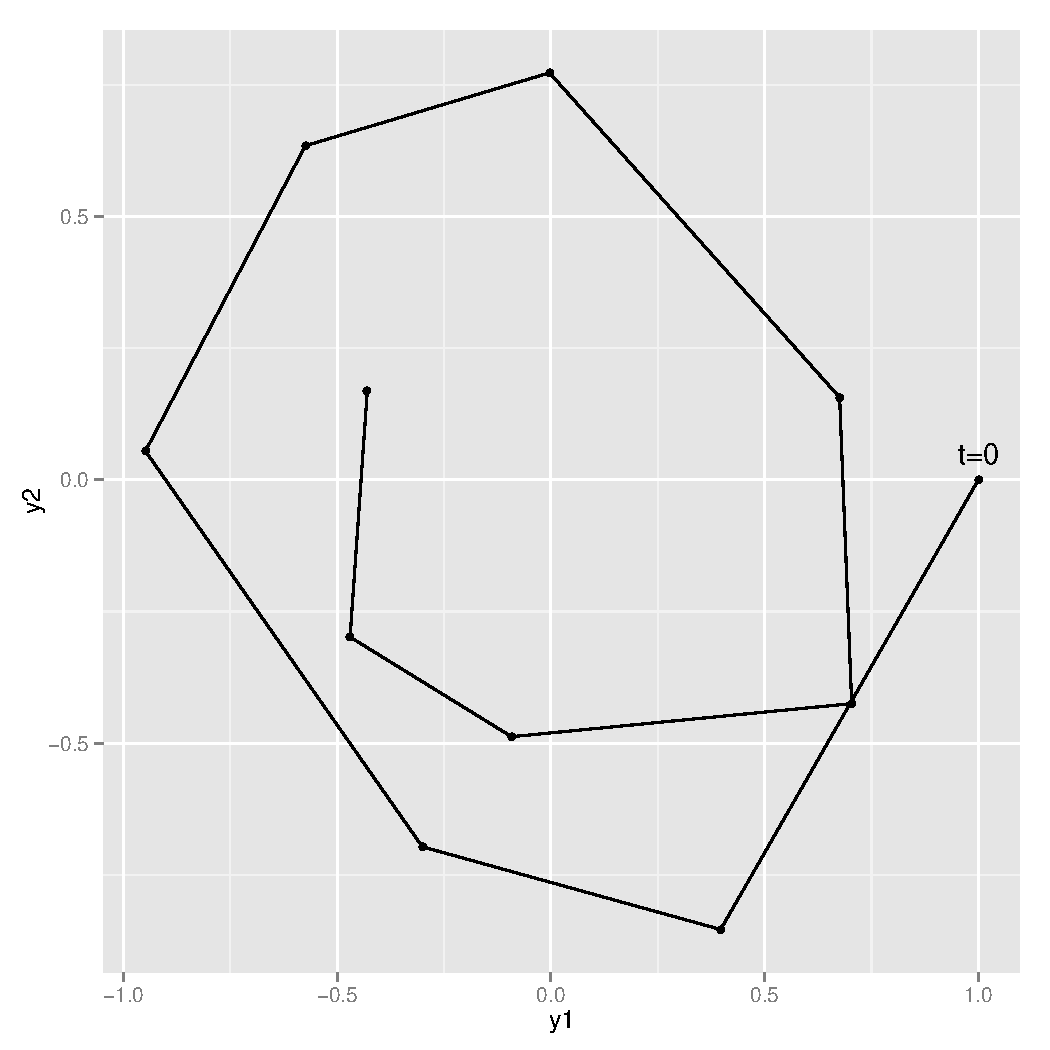
\includegraphics[height=2in]{img/sho-ode-trajectory.pdf}%
\end{center}
\vspace*{-0.25in}
\caption{\small\it Trajectory of the simple harmonic oscillator given
  parameter $\theta=0.15$ and initial condition $y(t=0) = (1,0)$ with
  additional independent\ $\distro{Normal}(0,0.1)$ measurement error
  in both dimensions.}%
\label{sho-trajectory.figure}
\end{figure}



\subsection{Simulating Noisy Measurements}

The data used to make this plot is derived from the Stan model to
simulate noisy observations given in \reffigure{sho-sim}.
%
\begin{figure}
\begin{stancode}
functions {
  real[] sho(real t,
             real[] y,
             real[] theta,
             real[] x_r,
             int[] x_i) {
    real dydt[2];
    dydt[1] = y[2];
    dydt[2] = -y[1] - theta[1] * y[2];
    return dydt;
  }
}
data {
  int<lower=1> T;
  real y0[2];
  real t0;
  real ts[T];
  real theta[1];
}
transformed data {
  real x_r[0];
  int x_i[0];
}
model {
}
generated quantities {
  real y_hat[T,2] = integrate_ode_rk45(sho, y0, t0, ts, theta, x_r, x_i);
  // add measurement error
  for (t in 1:T) {
    y_hat[t, 1] += normal_rng(0, 0.1);
    y_hat[t, 2] += normal_rng(0, 0.1);
  }
}
\end{stancode}
\vspace*{-0.2in}
\caption{\small\it Stan program to simulate noisy measurements from a
  simple harmonic oscillator.  The system of differential equations is
  coded as a function.  The system parameters \code{theta} and initial
  state \code{y0} are read in as data along with the initial time
  \code{t0} and observation times \code{ts}. The generated quantities
  block is used to solve the ODE for the specified times and then add
  random measurement error, producing observations \code{y\_hat}.
  Because the system is not stiff, the \code{rk45} solver is used.}\label{sho-sim.figure}
\end{figure}

This program illustrates the way in which the ODE solver is called in
a Stan program,
%
\begin{stancode}
y_hat = integrate_ode_rk45(sho, y0, t0, ts, theta, x_r, x_i);
\end{stancode}
%
This assigns the solutions to the system defined by function
\code{sho}, given initial state \code{y0}, initial time \code{t0},
requested solution times \code{ts}, parameters \code{theta}, real data
\code{x}, and integer data \code{x\_int}.  The call explicitly
specifies the Runge-Kutta solver (for non-stiff systems).

Here, the ODE solver is called in the generated quantities block to
provide a $10 \times 2$ array of solutions \code{y\_hat} to
which measurement error is added using the normal pseudo-random number
generating function \code{normal\_rng}.  The number of rows in the
solution array is the same as the size of \code{ts}, the requested
solution times.

\subsection{Data versus Parameters}

Unlike other functions, the integration functions for ODEs are limited
as to the origins of variables in their arguments.  In particular, the
time \code{t}, real data \code{x}, and integer data \code{x\_int} must
be expressions that only involve data or transformed data variables.
The initial state \code{y} or the parameters \code{theta} are the only
arguments which may involve parameters.


\subsection{Estimating System Parameters and Initial State}

Stan provides statistical inference for unknown initial states and/or
parameters.  The ODE solver will be used deterministically to produce
predictions, much like the linear predictor does in a generalized
linear model.  These states will then be observed with measurement error.

%
\begin{figure}
\begin{stancode}
functions {
  real[] sho(real t,
             real[] y,
             real[] theta,
             real[] x_r,
             int[] x_i) {
    real dydt[2];
    dydt[1] = y[2];
    dydt[2] = -y[1] - theta[1] * y[2];
    return dydt;
  }
}
data {
  int<lower=1> T;
  real y[T,2];
  real t0;
  real ts[T];
}
transformed data {
  real x_r[0];
  int x_i[0];
}
parameters {
  real y0[2];
  vector<lower=0>[2] sigma;
  real theta[1];
}
model {
  real y_hat[T,2];
  sigma ~ cauchy(0, 2.5);
  theta ~ normal(0, 1);
  y0 ~ normal(0, 1);
  y_hat = integrate_ode_rk45(sho, y0, t0, ts, theta, x_r, x_i);
  for (t in 1:T)
    y[t] ~ normal(y_hat[t], sigma);
}
\end{stancode}
\vspace*{-0.2in}
\caption{\small\it Stan program to estimate unknown initial conditions
  \code{y0} and system parameter \code{theta} for the simple harmonic
  oscillator with independent normal measurement
  error.}\label{sho-both.figure}
\end{figure}
%
A Stan program that can be used to estimate both the initial state and
parameter value for the simple harmonic oscillator given noisy
observations is given in \reffigure{sho-both}.  Compared to the
simulation model in \reffigure{sho-sim}, the model to estimate
parameters uses the \code{integrate\_ode} function in the model block
rather than the generated quantities block.  There are Cauchy priors on the
measurement error scales \code{sigma} and unit normal priors on the
components of parameter array \code{theta} and initial state parameter
array \code{y0}.  The solutions to the ODE are then assigned to an
array \code{y\_hat}, which is then used as the location in the
observation noise model as follows.
%
\begin{stancode}
y_hat = integrate_ode_rk45(sho, y0, t0, ts, theta, x_r, x_i);
for (t in 1:T)
  y[t] ~ normal(y_hat[t], sigma);
\end{stancode}
%
As with other regression-like models, it's easy to change the noise
model to be robust (e.g., Student-t distributed), to be correlated in
the state variables (e.g., with a multivariate normal distribution),
or both (e.g., with a multivariate Student-t distribution).

In this simple model with independent noise scales of 0.10, 10
observed data points for times $t = 1, ..., 10$ is sufficient to
reliably estimate the ODE parameter, initial state, and noise scales.


\section{Stiff ODEs}\label{stiff-ode.section}

A stiff system of ordinary differential equations can be roughly
characterized as systems presenting numerical difficulties for
gradient-based stepwise solvers.  Stiffness typically arises due to
varying curvature in the dimensions of the state, for instance one
component evolving orders of magnitude more slowly than another.%
%
\footnote{Not coincidentally, high curvature in the posterior of a
  general Stan model poses the same kind of problem for Euclidean
  Hamiltonian Monte Carlo (HMC) sampling.  The reason is that HMC is
  based on the leapfrog algorithm, a gradient-based, stepwise
  numerical differential equation solver specialized for Hamiltonian
  systems with separable potential and kinetic energy terms.}
%

Stan provides a specialized solver for stiff ODEs
\citep{CohenHindmarsh:1996,SerbanHindmarsh:2005}.  An ODE system is
specified exactly the same way with a function of exactly the same
signature.  The only difference is in the call to the integrator for
the solution; the \code{rk45} suffix is replaced with \code{bdf}, as in
%
\begin{stancode}
y_hat = integrate_ode_bdf(sho, y0, t0, ts, theta, x_r, x_i);
\end{stancode}
%

Using the stiff (\code{bdf}) integrator on a system that is not stiff
may be much slower than using the non-stiff (\code{rk45}) integrator;
this is because it computes additional Jacobians to guide the
integrator.  On the other hand, attempting to use the non-stiff
integrator for a stiff system will fail due to requiring a small step
size and too many steps.

\section{Control Parameters for ODE Solving}

The calls to the integrators shown above just used the default
control settings.  Both the non-stiff and stiff integrators allow
three additional arguments, all of which must be supplied if any of
them is required.
%
\begin{stancode}
y_hat = integrate_ode_bdf(sho, y0, t0, ts, theta, x_r, x_i,
                          rel_tol, abs_tol, max_steps);
\end{stancode}
%
The three control arguments are relative tolerance, absolute
tolerance, and maximum number of steps.   The default values for
relative and absolute tolerance are both \code{1e-6} ($10^{-6}$), and
the default maximum number of steps is \code{1e6} ($10^6$).

\subsection{Tolerance}

The relative and absolute tolerance control the accuracy of the
solutions generated by the integrator.  Relative tolerances are
relative to the solution value, whereas absolute tolerances is the
maximum absolute error allowed in a solution.

Smaller tolerances produce more accurate solutions.  Smaller
tolerances also require more computation time.

\subsubsection{Sensitivity Analysis}

The tolerances should be set low enough that setting them lower does
not change the statistical properties of posterior samples generated
by the Stan program.

\subsection{Maximum Number of Steps}

The maximum number of steps can be used to stop a runaway simulation.
This can arise in MCMC when a bad jump is taken, particularly during
warmup.  With the non-stiff solver, this may result in jumping into a
stiff region of the parameter space, which would require a very small
step size and very many steps to satisfy even modest tolerances.
